\documentclass{mcmthesis}
\mcmsetup{CTeX = false,    % 使用 CTeX 套装时,设置为 true
          tcn = {2520861}, problem = \textcolor{red}{C},
          sheet = true, titleinsheet = true, keywordsinsheet = true,
          titlepage = false, abstract = false}
        
\usepackage{newtxtext}     % \usepackage{palatino}
\usepackage[style=apa,backend=biber]{biblatex}
\addbibresource{reference.bib}

\usepackage{tocloft}
\usepackage{subcaption}
\usepackage{graphicx}
\usepackage{float}  %控制图片和表格的位置
\usepackage{indentfirst} %s首行缩进
\usepackage{threeparttable} %添加表格注释
\setlength{\cftbeforesecskip}{6pt}
%\setlength{\parindent}{2em} %全局首行缩进2字符
\renewcommand{\contentsname}{\hspace*{\fill}\Large\bfseries Contents \hspace*{\fill}}

\title{{\bf title}}
% \author{\small \href{http://www.latexstudio.net/}
%   {
\includegraphics[width=7cm]{mcmthesis-logo}}}
\date{\today}

\begin{document}
%%%%%%%%%%%%%%%%%%%%%%%%%%%%%%%%%%%%%%%摘要%%%%%%%%%%%%%%%%%%%%%%%%%%%%%%%%%%%%%%%%
\begin{abstract}

    During the 2024 Summer Olympics in Paris, there has been a surge in public interest in individual events and the medal rankings of various countries. Before each Olympic Games, a "virtual medal table" is created to predict the performance of different nations, but such predictions are typically based not only on historical medal data but also significantly influenced by the participating athletes. This article uses information such as the number and types of events a country participates in, project results, the host country, and specialty events to create a model.

    {\bf For issues one \& two}, we used {\bf K-Means clusterin} to categorize  the medal-winning countries into three types. We calculated the correlation between each country and different events using {\bf Pearson correlation coefficients}, in order to identify the country's signature events. Based on these three types of countries, we applied the {\bf LSTM} medal count training and prediction model.Using this model, we predicted the number of medals for each country at the 2028 Summer Olympics in Los Angeles.The model also found that the number and types of Olympic events have a significant impact on a country's medal count.

    {\bf For issue three}, we used a {\bf Random Forest} algorithm to build a model to predict which countries will win medals for the first time. The aim was to identify the key factors influencing the change in a country's medal count. We selected three feature variables: "number of participants," "number of participations," and "number of events," with "Will\_Earn\_Medal" as the target variable. We trained the model using a random forest regression model and used GridSearchCV to select the best hyperparameters, resulting in the optimal model configuration. We then calculated the probability of each country winning a medal.  the performance of the model was evaluated using {\bf confusion matrices} and {\bf ROC curves}, which showed high prediction accuracy.

    {\bf For issue four}, we used {\bf graph theory} and {\bf network flow} theory to quantitatively assess the influence of "great coaches" on a country's medal count. We established a directed network graph between coaches and countries, transforming the coach's impact on medals into node and edge flow relationships. The weight was calculated using the formula: $W=3\times \triangle G+2\times \triangle S+1\times \triangle B$. We then analyzed the coach's contribution to medals through total flow and bottleneck flow, providing countries with an optimized path for countries in selecting coaches and helping them to formulate more precise sports development strategies.
   
    {\bf For issue five}, during the modeling process for the above issues, we identified some strategies that can help National Olympic Committees to increase their medal count. For example, as women's participation increases, National Olympic Committees can focus on mixed-gender events to increase their chances of winning. If a country is the host nation, it can apply to add domestic advantage events, optimize infrastructure, and increase financial support to leverage the home advantage and increase medal count. For events that are not monopolized by a few countries, strong nations should analyze these events and invest in cultivating the next generation of athletes, while emerging sports nations can achieve breakthroughs in these non-monopolized events by precisely targeting projects and attracting in excellent coaches.   
    \begin{keywords}
        Prediction, LSTM, Random Forest, Olympic Games, Performance Modeling, Graph Theory
\end{keywords}
\end{abstract}


%%%%%%%%%%%%%%%%%%%%%%%%%%%%%%%%%%%%%%%目录%%%%%%%%%%%%%%%%%%%%%%%%%%%%%%%%%%%%%%%%
\maketitle

\tableofcontents
\thispagestyle{empty}

\newpage
%%%%%%%%%%%%%%%%%%%%%%%%%%%%%%%%%%%%%%%引言%%%%%%%%%%%%%%%%%%%%%%%%%%%%%%%%%%%%%%%%
\section{Introduction}
Faster, Higher, Stronger - Together.

\hfill ——International Olympic Committee

\subsection{Background}%%%%%%%%背景
The Paris Olympics attracted global attention, with the events attracting a lot of attention, especially the medal results of the athletes from different countries. Athletes from all over the world fought hard to get a place on the medals table. In addition to the traditional Olympic powerhouses and the hosts' medal race attracting much attention, there was also much discussion about some of the lower-ranked countries, such as Albania, Cape Verde, Dominica and Saint Lucia, who won their first ever medals at the Paris Games. However, there are still more than 60 countries that have failed to collect Olympic medals.

Looking back at history, countries' medal performances in the Olympics show a certain pattern. Before each Olympics, there will be a ‘virtual medal table’ to predict the performance of countries. For example, before the Paris Olympics, Nielsen Gracenote released its final Virtual Medal Table (VMT) predictions for the 2024 Olympics. So what specific factors do such predictions rely on? The fact is that medal predictions are usually made near the start of the Olympic Games by building mathematical models that take into account known athlete participation plans and analysing past gold and total medal counts, in order to predict future medal rankings. Such forecasts are not only valuable to sports analysts, researchers and policymakers, but also help countries to better grasp the trends affecting Olympic performance.

\subsection{Restatement of the Problem}%%%%%%%%问题重述
Given the background information and constraints of the problem, we must complete the following tasks:
\begin{itemize}
\item Task 1: Predict the medal table for the 2028 Summer Olympics in Los Angeles, USA, outputting the countries that will perform better as well as those that will perform worse.
\item Task 2: Analyse the relationship between the number and type of Olympic sports and the number of medals, output the most important sports for each country and analyse the impact of the host country's choice of sports on performance.
\item Task 3: For countries that have not yet won a medal, predict the probability that they will win their first medal at the next Olympic Games and provide an estimate of the probability of this prediction
\item Task 4: Explore the impact of the Great Coach effect on team sports, looking for evidence of the impact of the Great Coach effect and estimating the strength of the effect. Finally, select three countries to recommend sports that are worth investing in and estimate their impact.
\item Task 5: Provide original insights into Olympic medal counts and explain how these insights inform the Olympic Committee's decision-making.
\end{itemize}

\subsection{Our Work}%%%%%%%%文章分析


%%%%%%%%%%%%%%%%%%%%%%%%%%%%%%%%%%%%%%%假设%%%%%%%%%%%%%%%%%%%%%%%%%%%%%%%%%%%%%%%%%%%
\section{Assumptions and Justification}

%%%%%%%%%%%%%%%%%%%%%%%%%%%%%%%%%%%%%%%符号说明%%%%%%%%%%%%%%%%%%%%%%%%%%%%%%%%%%%%%%%%
\section{Notations}

%%%%%%%%%%%%%%%%%%%%%%%%%%%%%%%%%%%%%%%数据处理%%%%%%%%%%%%%%%%%%%%%%%%%%%%%%%%%%%%%%%%
\section{Data Cleaning}
The study began with a systematic cleaning and pre-processing of the raw data.

In terms of athlete data processing, we performed operations such as removing duplicate entries, handling missing values, standardizing, and converting data types on the summerOly\_athletes.csv dataset, which contains basic athlete information (name, team, NOC, sport, events, medals, etc.). In addition, we found that the presence of spaces in the string text affected the subsequent data analyses, so we used str.strip() to remove leading and trailing spaces, and str.replace() to remove internal spaces. We also deleted invalid information and performed reverse processing on the summerOly\_programs.csv dataset for easier future use

In the NOC (National Olympic Committee) validation session, we used the athletes dataset as the primary reference source for valid NOCs and cross-validated it with the hosts and medals datasets. To ensure data consistency, we removed NOC entries from the hosts and medals datasets that were not present in the athletes dataset. This step provided a reliable foundation for subsequent data analyses.

To ensure data quality, we performed strict validation and quality checks, including ensuring consistency of NOC codes across all datasets, verifying year ranges and temporal continuity, and checking logical constraints such as the number of gold medals not exceeding the total number of medals. Care was taken to maintain the integrity of the data at all times during the dataset consolidation process.

Finally, we performed necessary additional transformations on the data, created an aggregated view of historical performance, unified the data format of each dataset, and prepared a standardised data structure for subsequent analysis and modelling. Through this series of rigorous data cleansing processes, we ensured the consistency, completeness and normality of the datasets, laying a solid foundation for the predictive modelling phase. These steps not only improve the data quality, but also enhance the reliability of the results of subsequent analyses.


%%%%%%%%%%%%%%%%%%%%%%%%%%%%%%%%%%%%%%%模型结构%%%%%%%%%%%%%%%%%%%%%%%%%%%%%%%%%%%%%%%%
\section{TASK1\&2: Medal Count Prediction Based on LSTM}

\subsection{Data Analysis}
First, we constructed a Feature Correlation Matrix for countries that have previously won medals to identify the advantage sports of some nations. Subsequently, we created contingency tables for each country, including features such as the year of medal wins, total medal count, gold medal count, host status, number of participants, number of events participated in, total events established by the host, and events from past editions. Finally, we used K-Means clustering to classify countries that have previously won medals into three categories, which serves as the basis for building separate predictive models for different types of Olympic nations.
\subsubsection{Correlation Matrix Analysis Based on Pearson Correlation}
\begin{itemize}
\item {\bf Step 1: Data Preparation:}Align the medal count dataset with the event dataset to ensure that each row represents the number of medals a country won in a specific event.
\item {\bf Step 2: Pearson Correlation:}The Pearson correlation coefficient is suitable for analyzing data that follows a continuous normal distribution. The calculation formula is as follows:

\begin{equation} \label{13}
    \rho(x,y)=\frac{\mathrm{cov}(x,y)}{\sigma(x)\cdot\sigma(y)}=\frac{E[(x-\mu_x)(y-\mu_y)]}{\sigma(x)\cdot\sigma(y)}
\end{equation}

\item {\bf Step 3: Correlation Calculation}:For each country, we combined the number of medals won by that country in various events with the total number of medals awarded across different Olympic events to calculate the Pearson correlation coefficient. The Pearson correlation coefficient quantifies the strength of the relationship between variables. The intensity of variable correlations is shown in Figure 1. We visualized the resulting correlation matrix and, taking China as an example, generated a heatmap as shown in Table 1.

\begin{table}[H]
    \centering
    \caption{Variable Correlation Strength}
    \vspace{-0.3pt}
    \begin{tabularx}{\textwidth}{>{\centering\arraybackslash}X>{\centering\arraybackslash}X>{\centering\arraybackslash}X>{\centering\arraybackslash}X>{\centering\arraybackslash}X>{\centering\arraybackslash}X}
        \toprule[2pt]
        \textbf{Correlation Strength}  & \textbf{Very Strong Correlation}     & \textbf{Strong Correlation} & \textbf{Moderate Correlation} & \textbf{Weak Correlation} & \textbf{Very Weak or No Correlation} \\ 
        \midrule[1pt]
        \textbf{Absolute value of correlation coefficient} & \makebox[2cm]{0.8--1} & \makebox[2cm]{0.6--0.8} & \makebox[2cm]{0.4--0.6} & \makebox[2cm]{0.2--0.4} & \makebox[2cm]{0--0.2} \\ 
        \bottomrule[2pt]
    \end{tabularx}
    \label{tab:feature_importance}
\end{table}

\begin{figure}[H]
    \centering
    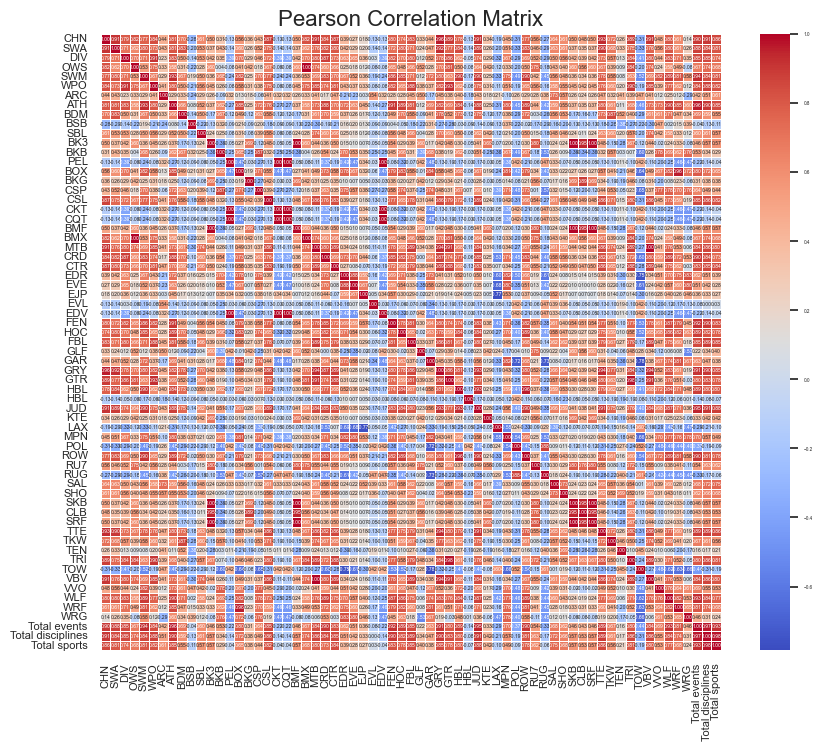
\includegraphics[width=10cm]{graph/heatmap.png}
    \caption{Heatmap of China} \label{Figure 4}
\end{figure}

\begin{figure}[H]
    \centering
    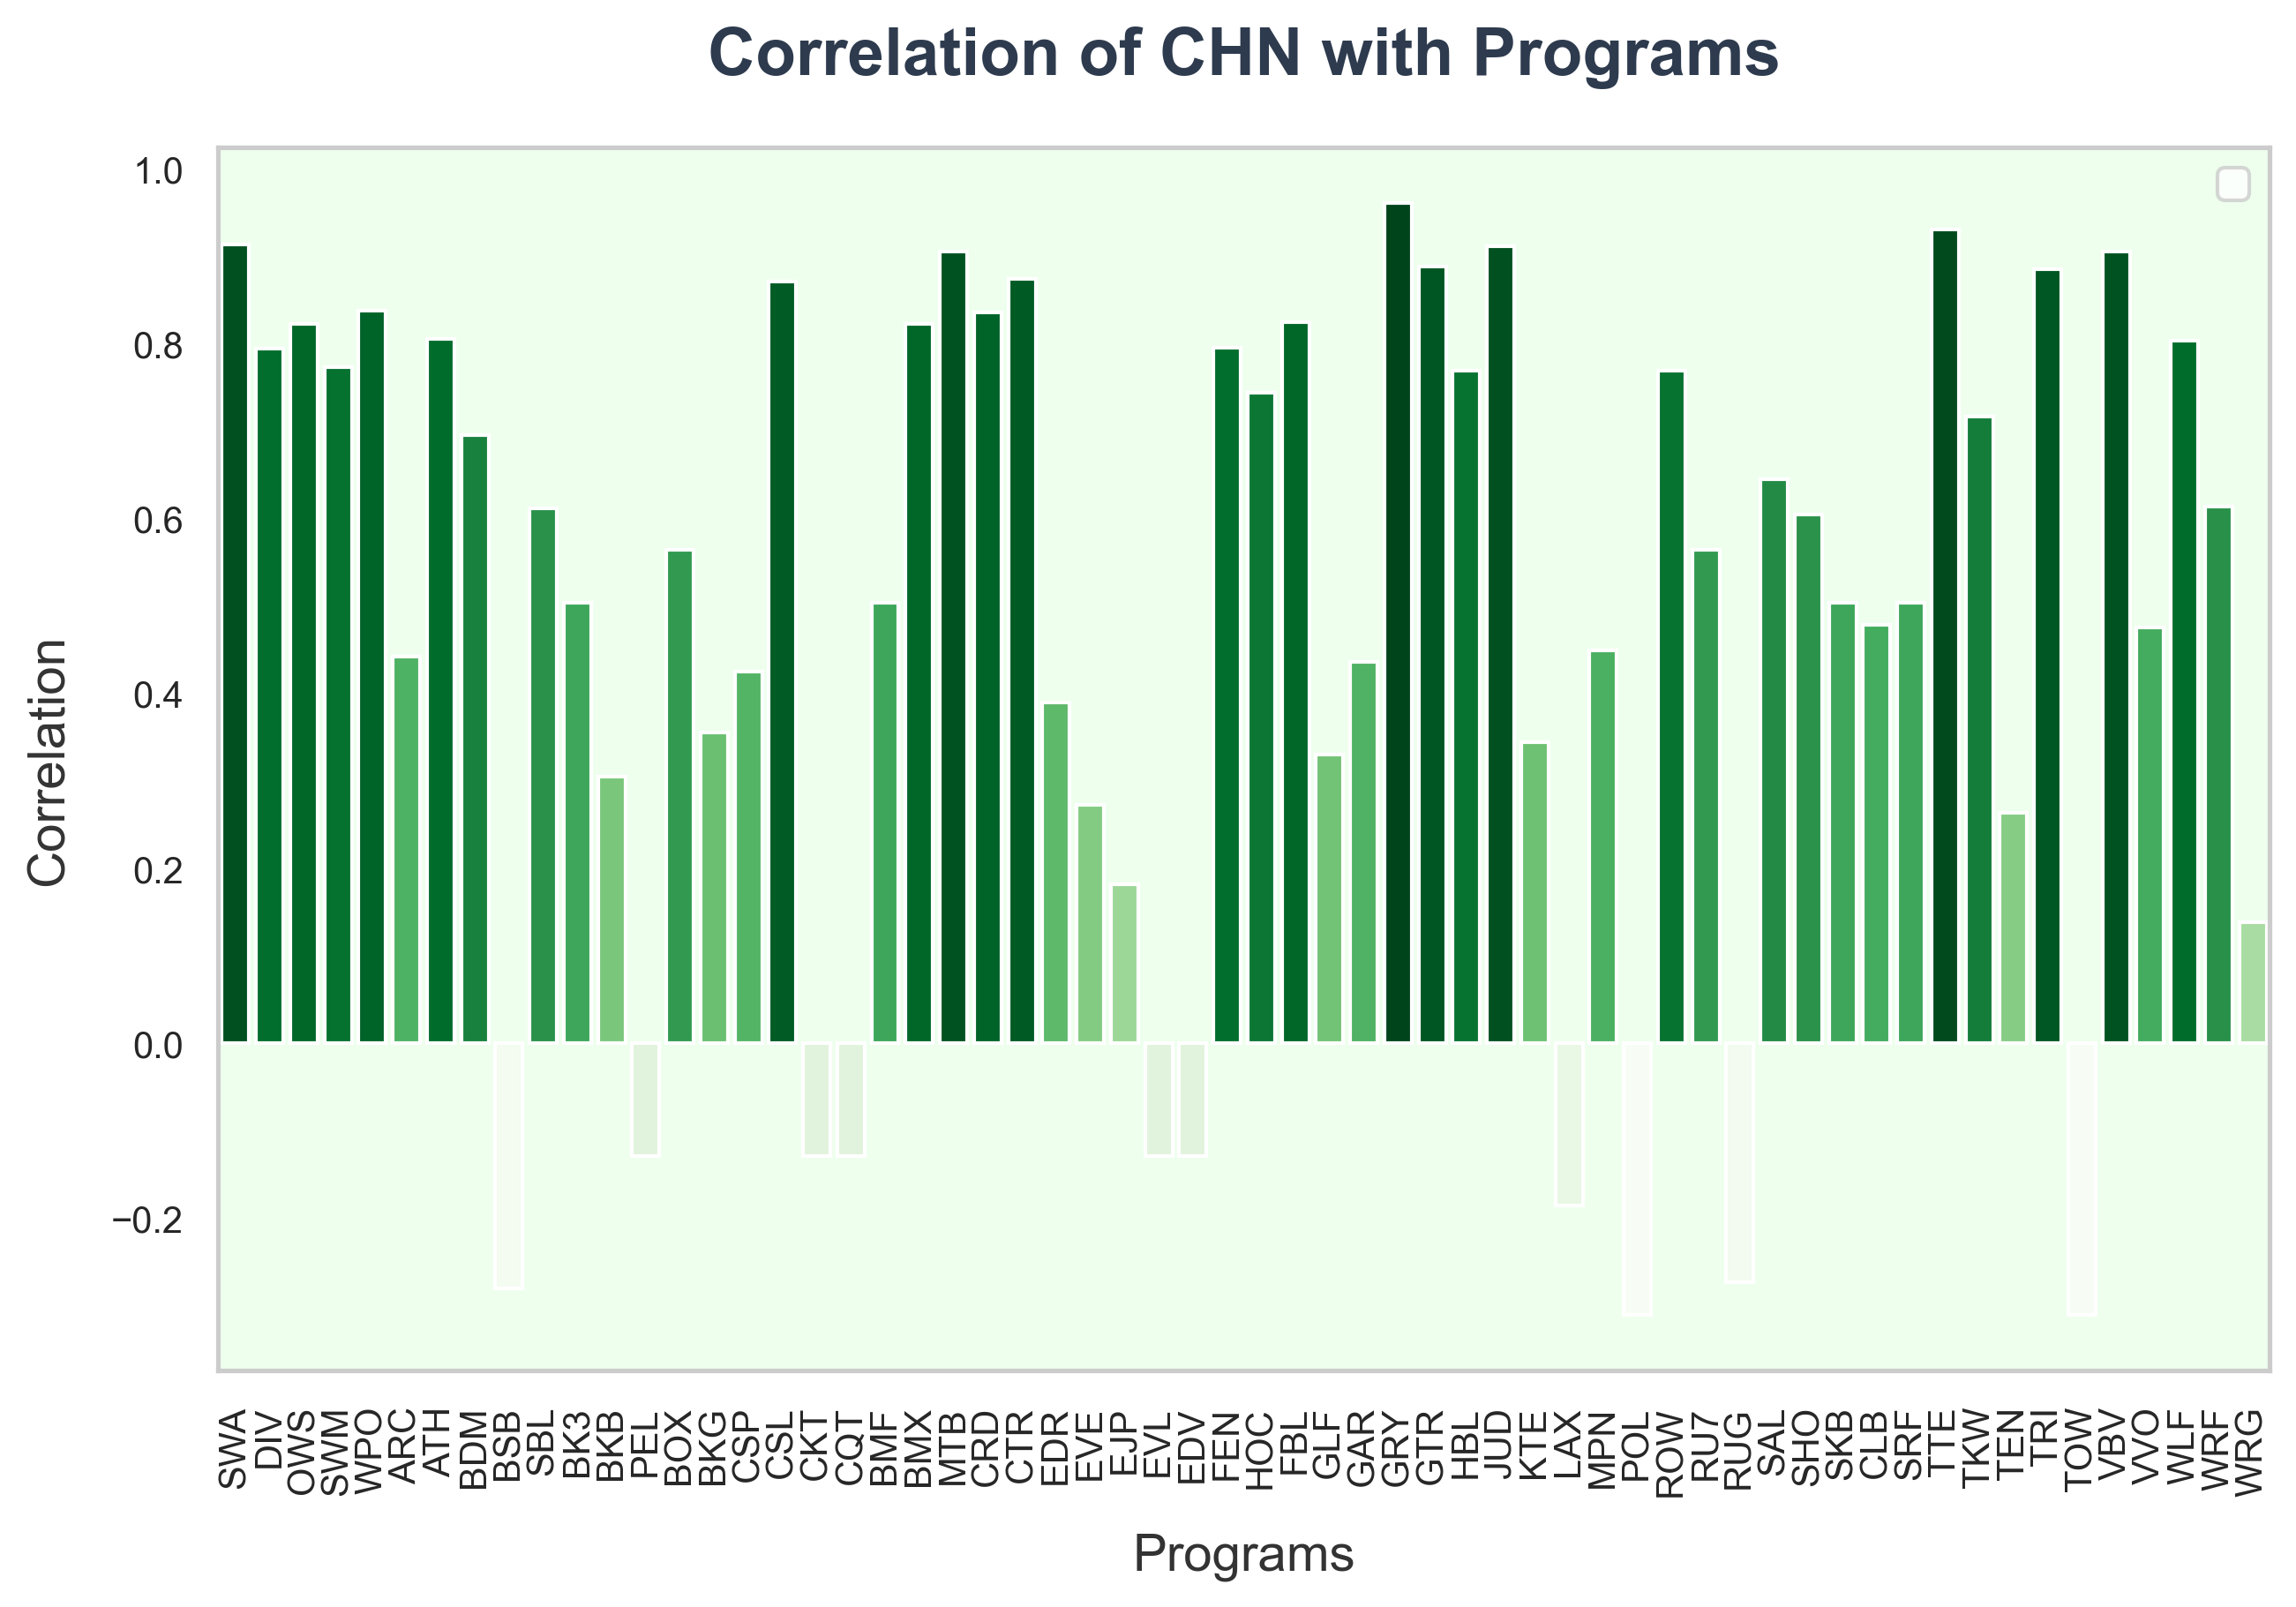
\includegraphics[width=12cm]{graph/Correlation of CHN with Programs.png}
    \caption{Correlation of CHN with Programs} \label{Figure 4}
\end{figure}

\item {\bf Step 4: Analyzing Advantage Sports: }Return a series containing the top three independent variables with the highest correlation coefficients. These represent the three events that most significantly impact a country's total medal count, which are identified as the country's advantage sports. Taking China as an example, the results and the heatmap above indicate that China's advantage sports are gymnastics, table tennis, and diving.
\item {\bf Step 5: Constructing Contingency Tables:} Create a contingency table for each country, including the year of medal wins, host status, total medal count, gold medal count, total number of events established by the host, number of events participated in, advantage sports, and average medals won.

\end{itemize}

\subsubsection{A Classification Model for Medal-Winning Countries Based on K-Means}

\begin{figure}[H]
    \centering
    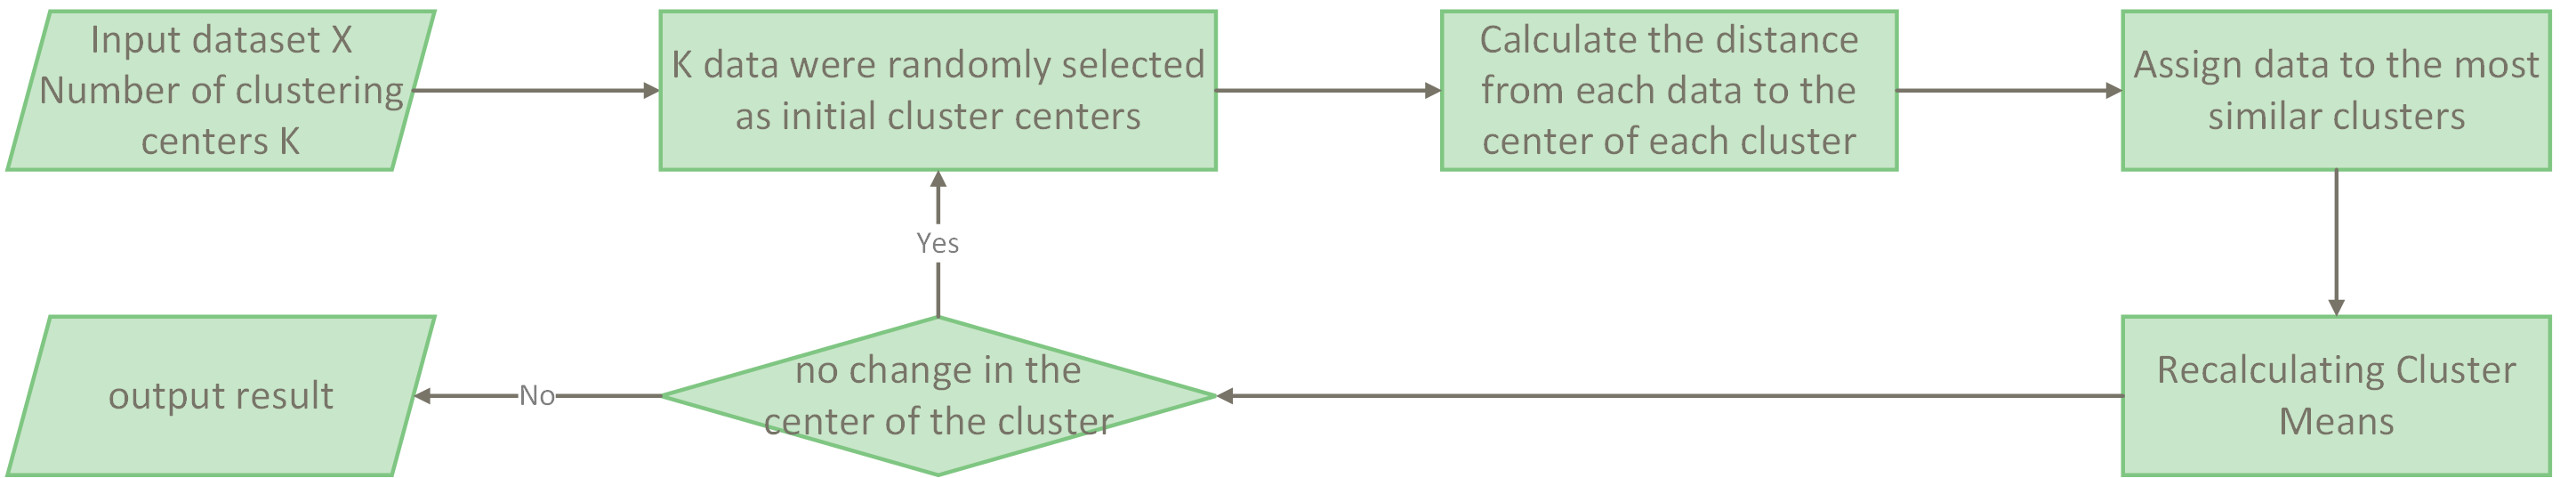
\includegraphics[width=12cm]{graph/K-means.png}
    \caption{K-Means Flowchart} \label{Figure 4}
\end{figure}
To achieve accurate medal predictions, it is essential to scientifically classify participating countries. Before categorizing national teams based on medal-winning stability, we first need to define stability. For this purpose, we use two key dimensions: NOC participation frequency and diversity of sports events. Based on these dimensions, we apply the K-Means clustering algorithm to classify countries.

1.	Feature Construction

\qquad NOC Participation Frequency: $f_{\text{participation}}$ = $\text{count(NOC)}$

\qquad Sports Diversity Index: $f_{\text{diversity}}$ = $\text{unique\_count(Sports)}$

\qquad Feature Normalization: $X'$ = $\text{MinMaxScaler}$

2.	Clustering Implementation
Achieved by minimizing the within-cluster sum of squares (WCSS) objective function.
\begin{equation} \label{}
    d(x_i,C_j^{(r)})=\sqrt{\sum_{l=1}^d(x_{il}-C_{jl}^{(r)})^2}
\end{equation}
\begin{equation}\label{}
    C_j^{(r+1)}=\frac{1}{|S_j^{(r)}|}\sum_{x_i\in S_j^{(r)}}x_i
\end{equation}
First, we calculated the occurrence frequency of each NOC in the dataset athletes\_with\_gold\_medal and the number of unique sports associated with each NOC. The data for NOC and sports were normalized using MinMaxScaler, and the two features were merged into a single dataset for K-Means clustering.

During the clustering process, it was observed that data points for the United States exhibited significant outlier characteristics. This was primarily due to the U.S. far exceeding other countries in both NOC participation frequency and the number of sports, resulting in a distinct data distribution. This uniqueness reflects the comprehensive dominance of the U.S. in the Olympics but also posed challenges for clustering analysis. To ensure the rationality of the clustering results, appropriate modifications to the clustering method are required.

\begin{figure}[H]
    \centering
    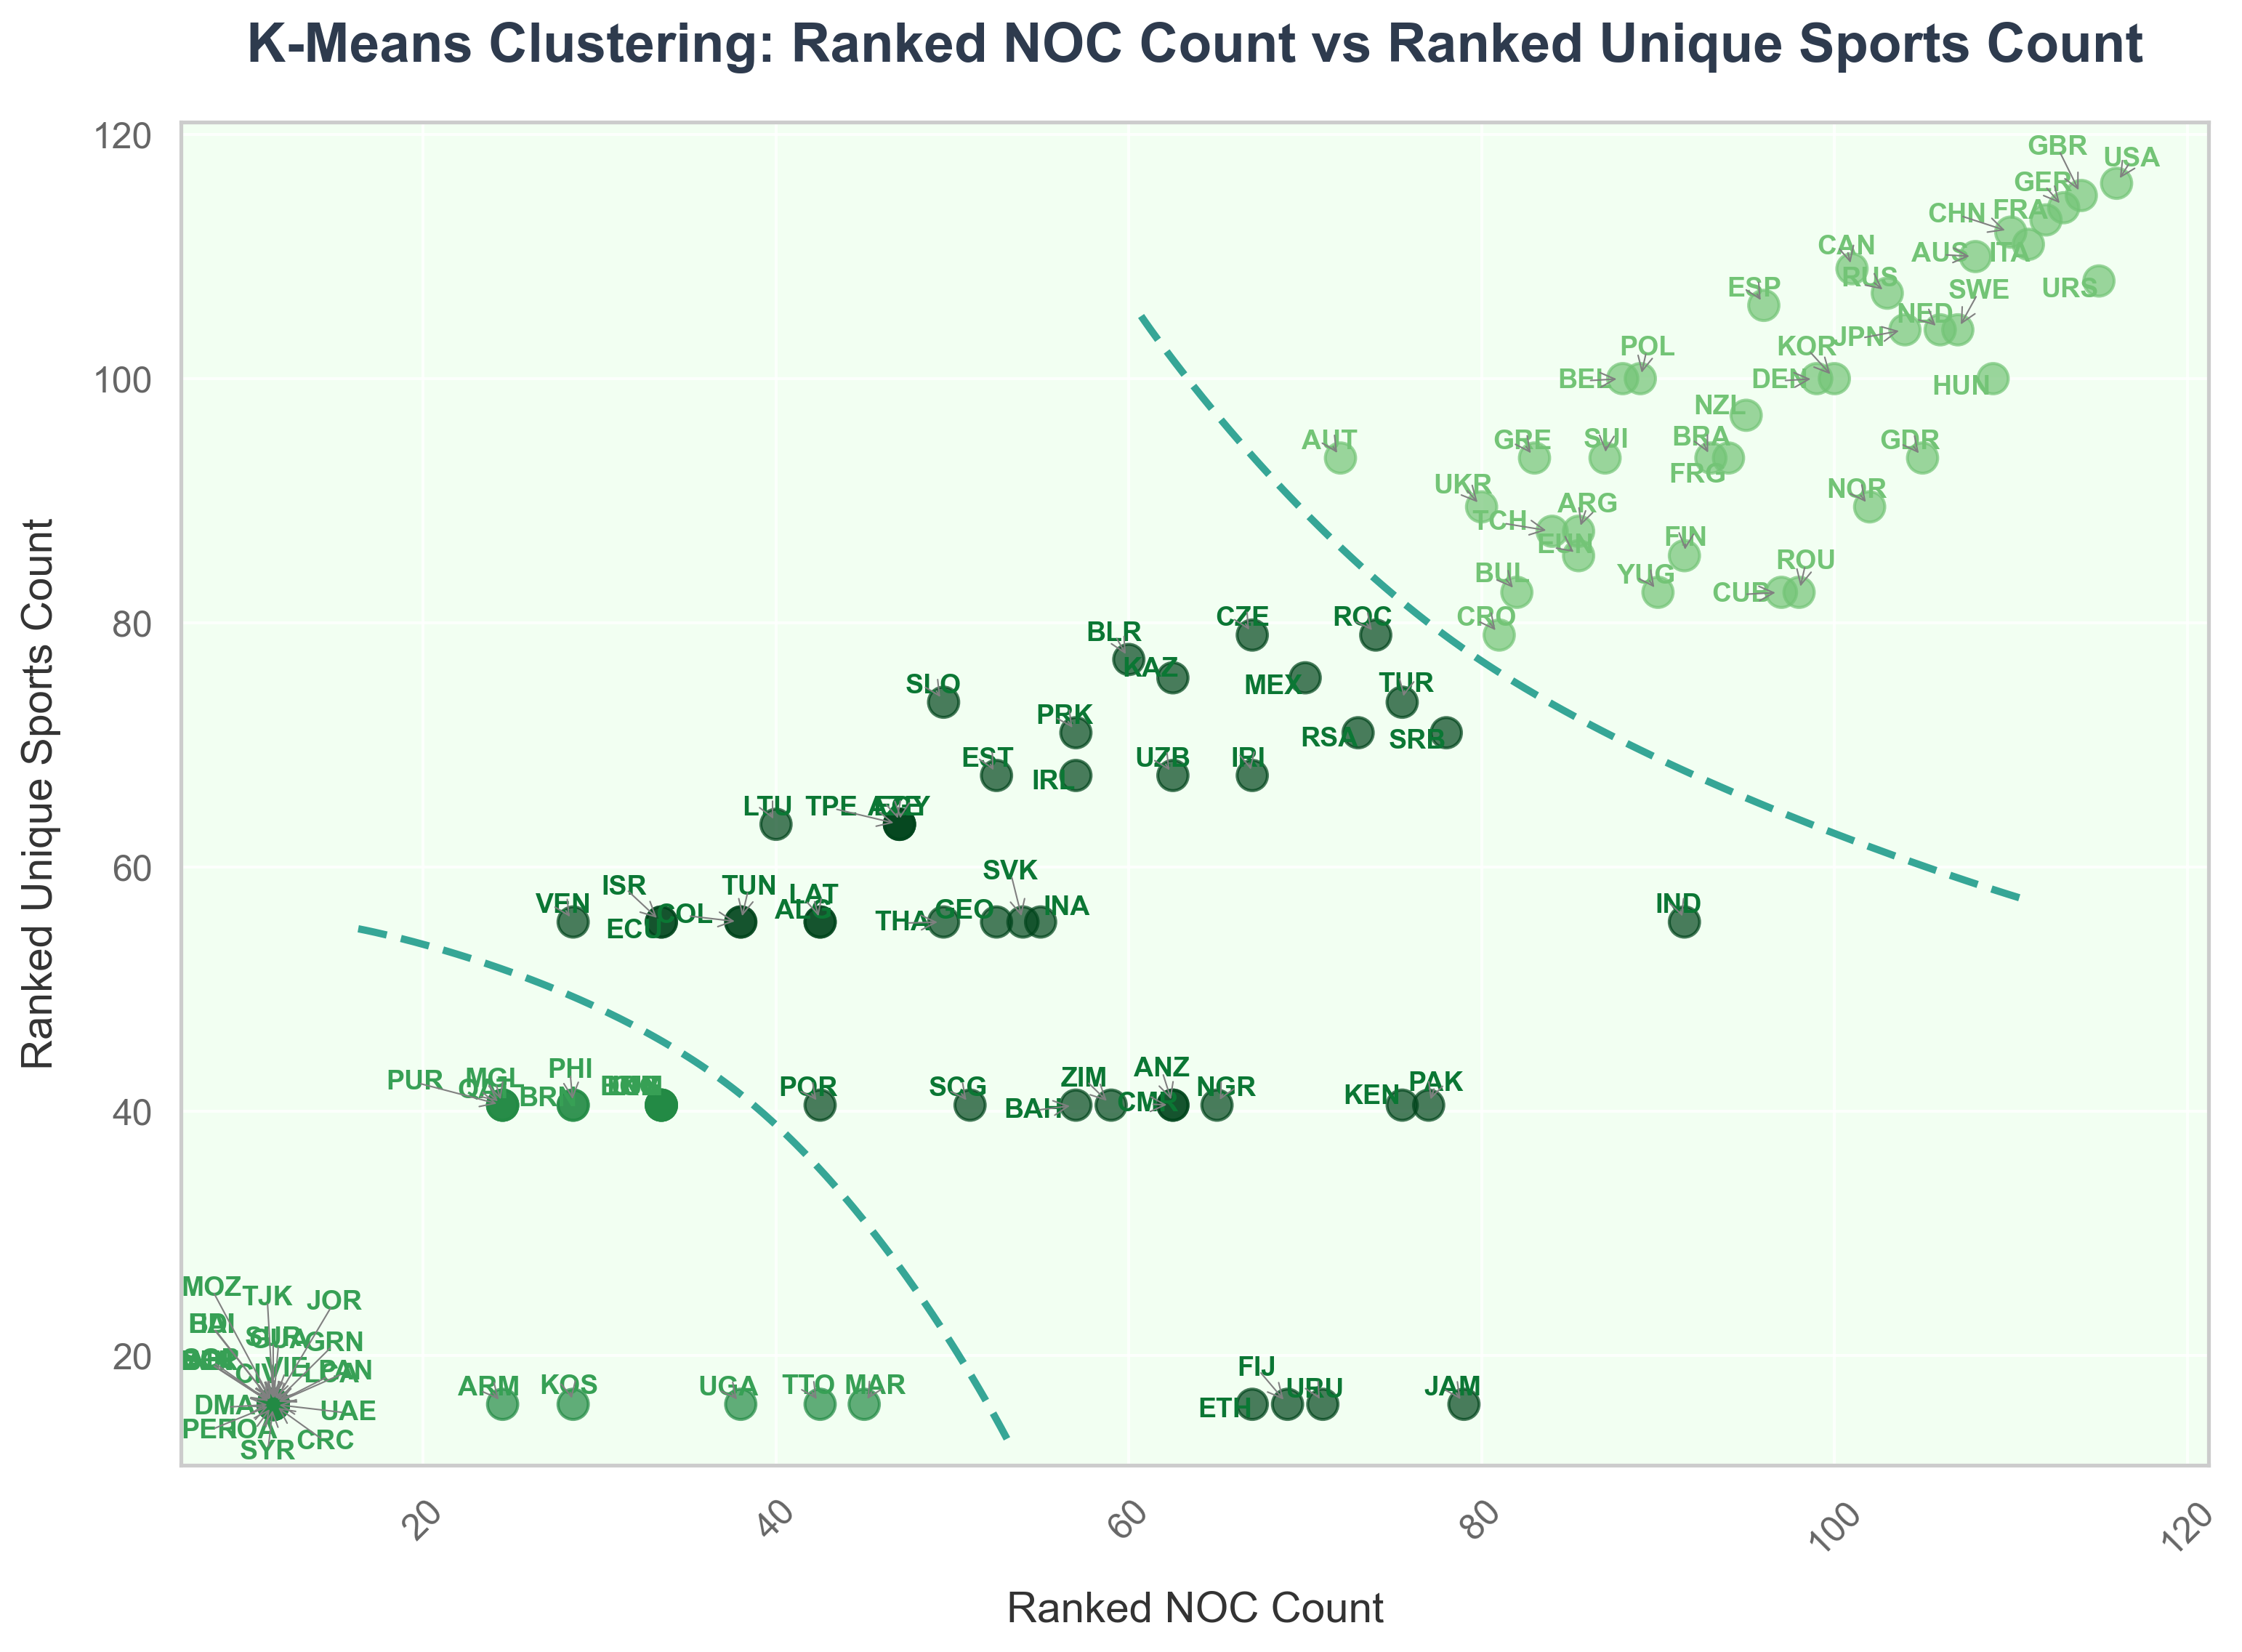
\includegraphics[width=10cm]{graph/K-Means Clustering Redraw.png}
    \caption{K-Means Clustering Diagram} \label{Figure 4}
\end{figure}

We decided to use the rankings of NOC and Sport occurrence frequencies as the basis for clustering and dividing countries into different groups. Additionally, during the model selection phase, we experimented with both K-Means and DBSCAN to cluster the athletes\_with\_medal and athletes\_with\_gold\_medal datasets. The results showed that clustering the athletes\_with\_gold\_medal dataset using the K-Means model yielded the best performance.

Based on Figure 4, we obtained our final clustering results:Category 1 includes 37 countries that have won gold medals, Category 2 includes 36 countries, and Category 3 includes 43 countries.


\begin{table}[htbp]
    \centering
    \caption{Group and Feature Description}
    \begin{tabular}{@{}p{5cm}p{10cm}@{}}
        \toprule[2pt]
        \textbf{Group} & \textbf{Feature Description} \\
        \midrule[1pt]
        Cluster-1 (Olympic Powerhouses) & 
        High participation frequency \\
        & Diverse event distribution \\
        & Stable medal-winning ability \\
        \addlinespace
        Cluster-2 (Developing Sports Nations) & 
        Moderate participation frequency \\
        & Relatively concentrated event distribution \\
        & Fluctuating medal performance \\
        \addlinespace
        Cluster-3 (Unstable Nations) & 
        Low participation frequency \\
        & Highly unstable medal performance \\
        & Strong reliance on advantage sports \\
        \bottomrule[2pt]
    \end{tabular}
\end{table}

\subsection{Model Selection}
Considering that the data we processed is associated with specific time points and measured at uniform intervals (every four years), we decided to use time series analysis to predict medal counts.

Traditional time series forecasting methods, such as the commonly used Auto-Regressive Integrated Moving Averages (ARIMA), rely solely on a single time series data source. However, predicting medal counts typically requires incorporating multiple variables beyond just historical medal counts.

With the development of machine learning and artificial intelligence, various deep learning algorithms have been applied to time series forecasting. For example, Long Short-Term Memory Networks (LSTM) can address the limitations of Recurrent Neural Networks (RNNs) in capturing long-term cycles and seasonal patterns. In each time step of an LSTM, there is a memory cell, which provides the network with selective memory functionality. This allows LSTM to determine which content to retain at each time step.

Moreover, LSTM can handle multivariate analysis, and its ability to analyze multiple variables aligns well with the three-category grouping of countries based on K-Means clustering. This makes it possible to adopt differentiated variable weighting strategies for different types of countries.

\subsection{Long and Short Term Memory Network}
The study employs an LSTM network as the core predictive model, consisting of three key components: the Forget Gate, Input Gate, and Output Gate. The Forget Gate $f_t$ controls the retention of historical information, the Input Gate $i_t$ manages the updating of new information, and the Output Gate $o_t$ determines the output of information. Together, these three components form a complete memory mechanism:
\begin{equation}\label{}
    f_t=\sigma(W_f\cdot[h_{t-1},x_t]+b_f)
\end{equation}
\begin{equation}\label{}
    i_t=\sigma(W_i\cdot[h_{t-1},x_t]+b_i)
\end{equation}
\begin{equation}\label{}
    o_t=\sigma(W_o\cdot[h_{t-1},x_t]+b_o)
\end{equation}
Here, $h_t$ represents the hidden state at time $t$, and $x_t$ is the input vector.

\begin{figure}[H]
    \centering
    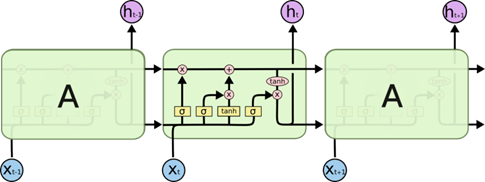
\includegraphics[width=12cm]{graph/workflow.png}
    \caption{Workflow Diagram of the LSTM Mechanism} \label{Figure 4}
\end{figure}

\subsection{Implementation of LSTM}
We performed normalization on the data to reduce the impact of scale differences between features and ensure stability during the training process. Subsequently, we created the input dataset using a sliding window approach, segmenting the original medal data based on the time window. The time step was set to 20, meaning each year's medal count is related to the data from the previous 20 years.
\begin{figure}[H]
    \centering
    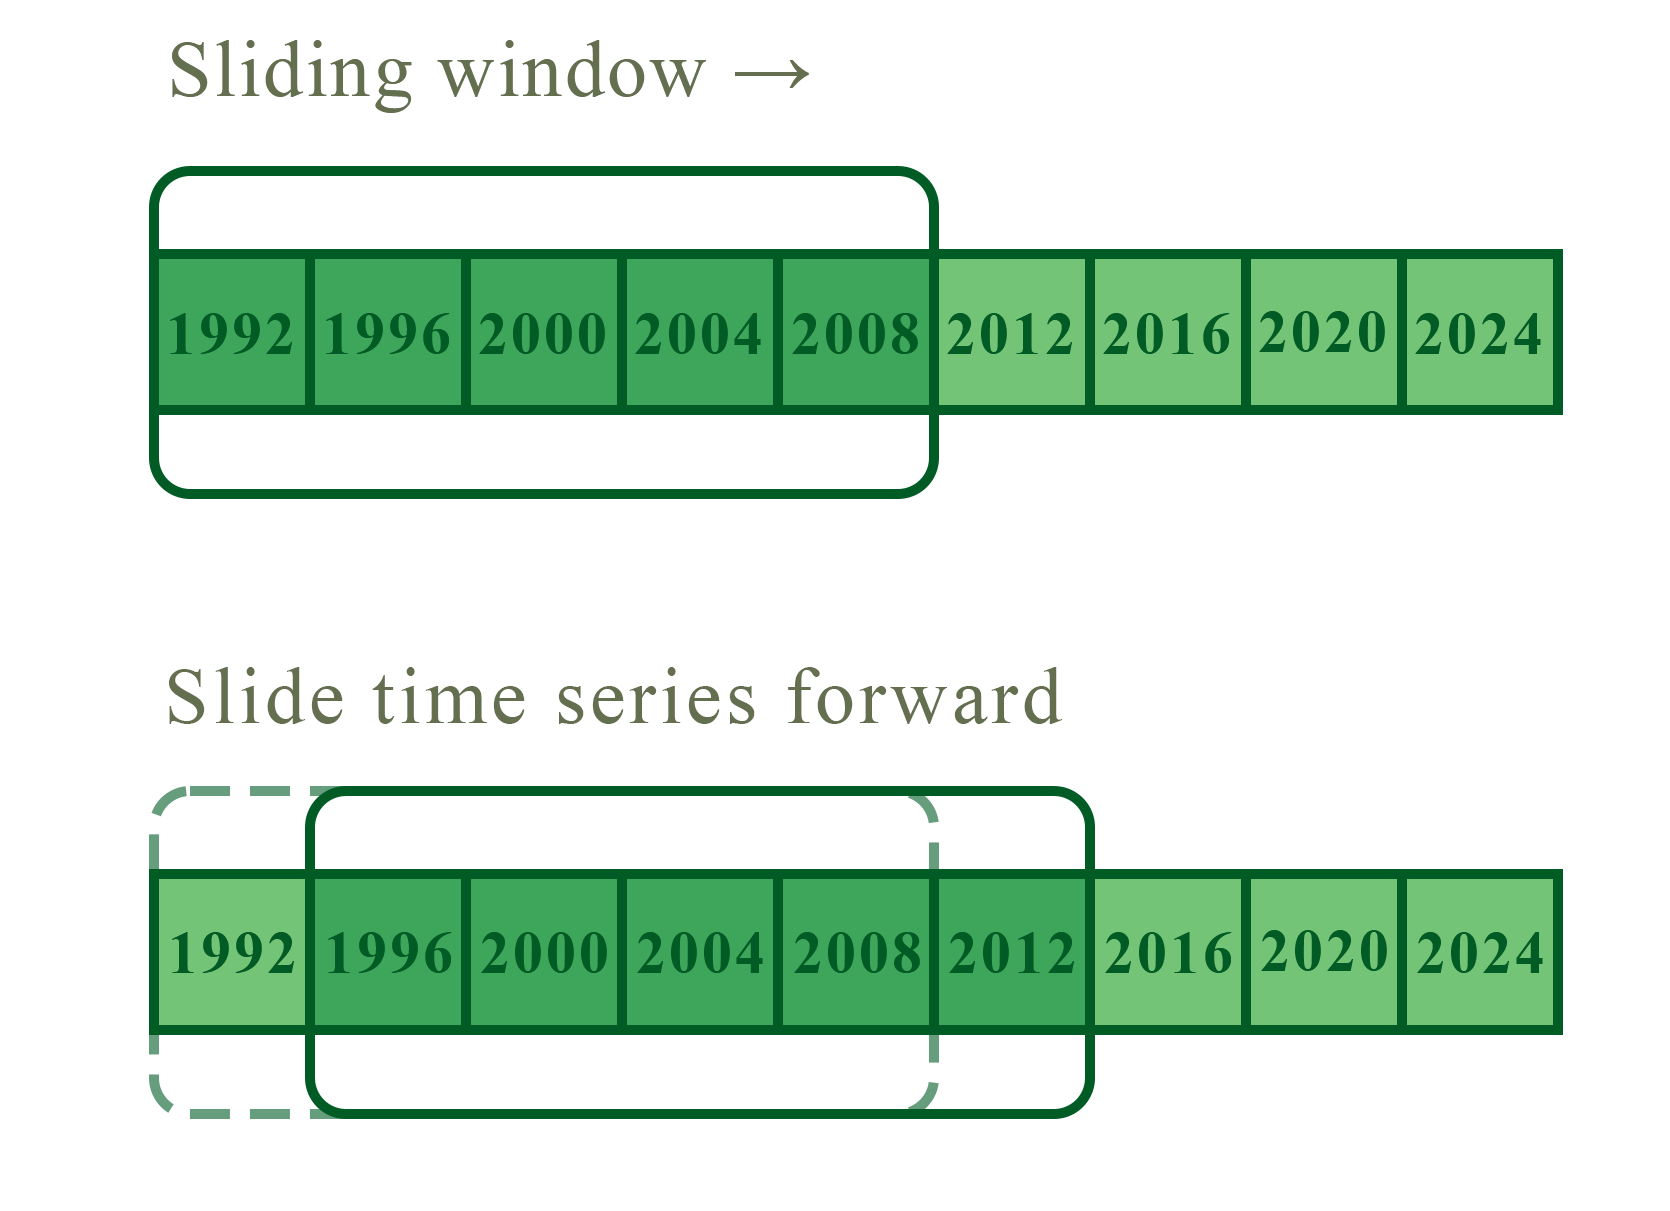
\includegraphics[width=12cm]{graph/sliding_window.png}
    \caption{Sliding Window} \label{Figure 4}
\end{figure}

\subsubsection{Quantifying the Impact of Host Countries}
We used the Ordinary Least Squares (OLS) method, taking the total medal count as the dependent variable and host country and events as independent variables. The model yielded an $R^{R}$ of 0.758 and an adjusted $R^{R}$ of 0.756, both relatively high, indicating that the model explains over 75.8\% of the variation in total medal counts, demonstrating a good fit. The p-value for the independent variable "host country" is less than 0.05, indicating high significance and statistical validity, with a substantial impact on the total medal count.


\begin{table}[H]
    \centering
    \caption{Results of the Ordinary Least Squares Method}
    \begin{tabularx}{\textwidth}{>{\centering\arraybackslash}X>{\centering\arraybackslash}X>{\centering\arraybackslash}X>{\centering\arraybackslash}X>{\centering\arraybackslash}X}
        \toprule[2pt]
            a&\textbf{coef} & \textbf{std err} & \textbf{t} & \textbf{P>|t|}  \\
        \midrule[1pt]
        const & 10.4972 & 5.090 & 2.062 & 0.041 \\ 
        host & 26.9574 & 4.975 & 5.419 & 0.000 \\ 
        sport & 1.3783 & 0.226 & 6.103 & 0.000 \\ 
        \bottomrule[2pt]
        \end{tabularx}
\end{table}

\subsubsection{Building the LSTM Model}
As mentioned earlier, we used K-Means clustering to divide medal-winning countries into three categories:
\begin{itemize}
\item {\bf Category 1}: Established Olympic powerhouses with frequent participation and a wide range of events, such as the United States and China.
\item {\bf Category 2}: Countries with frequent participation but inconsistent performance, such as Luxembourg and Singapore.
\item {\bf Category 3}: Countries with infrequent participation and unstable performance, such as India and Jamaica.
\end{itemize}

For each country, we constructed a time series that includes variables such as annual medal count, gold medal count, host status, number of participants, number of events participated in, number of events established by the host, and the distribution of awards for each event in previous Olympics. Among these, medal count, gold medal count, host status, number of participants, number of events, and the number of events established by the host were treated as the country’s historical predictors of medal performance. The product of the award distribution for each event and the Pearson correlation coefficient was used to represent the country's advantage sports.

Weighting strategies by category:
\begin{itemize}
    \item {\bf Category 1}: These countries are typically strong and have won medals across a wide range of events, without relying on advantage sports. For such countries, since the influence of being the host nation is significant, we multiplied this factor by the influence derived from the OLS regression, distributed the weights of other historical predictors evenly, and set the weight for advantage sports to zero.
    \item {\bf Category 2}:For these countries, medal predictions depend on both past participation and performance, as well as certain advantage sports. For these nations, all variables were included, and the weight for advantage sports was calculated as $t{weight} = (1-w) \times \text{Pearson Correlation Coefficient}$
    \item {\bf Category 3}:  These countries have few appearances and very low historical medal counts, making predictions akin to estimating the probability of winning medals. As past participation data is less relevant, only advantage sports were considered, and the weight of historical data was set to zero.
\end{itemize}
Model Architecture Design:

We employed an LSTM layer with 50 memory cells as the primary feature extractor, capable of effectively capturing both short- and long-term dependencies within Olympic cycles. Following the LSTM layer, a fully connected layer was used for feature integration. Finally, the output layer, consisting of two neurons, was designed to predict total medal count and gold medal count, respectively.

Considering that recent Olympic performance is more indicative of future outcomes, we introduced a temporal decay weighting mechanism in the model. This allowed the model to retain historical information while focusing more on recent data trends.

\subsection{Prediction Interval from the Result}
We calculated the prediction intervals through multiple training and testing iterations for each country's model. Each country's model was trained and predicted 10 times to obtain the distribution of the final results. After removing outliers from the results, the maximum and minimum values were taken as the range of medal counts or the range of winning probabilities. The average loss for a country's model was calculated as the model's loss, and the overall model performance was determined by averaging the losses of all countries' models.

\begin{figure}[H]
    \centering
    % 减少顶部间距
    \vspace{-0.15in}
    
    % 第一行两张图片
    \begin{minipage}{1\linewidth}
        \subfloat[]{\label{USA}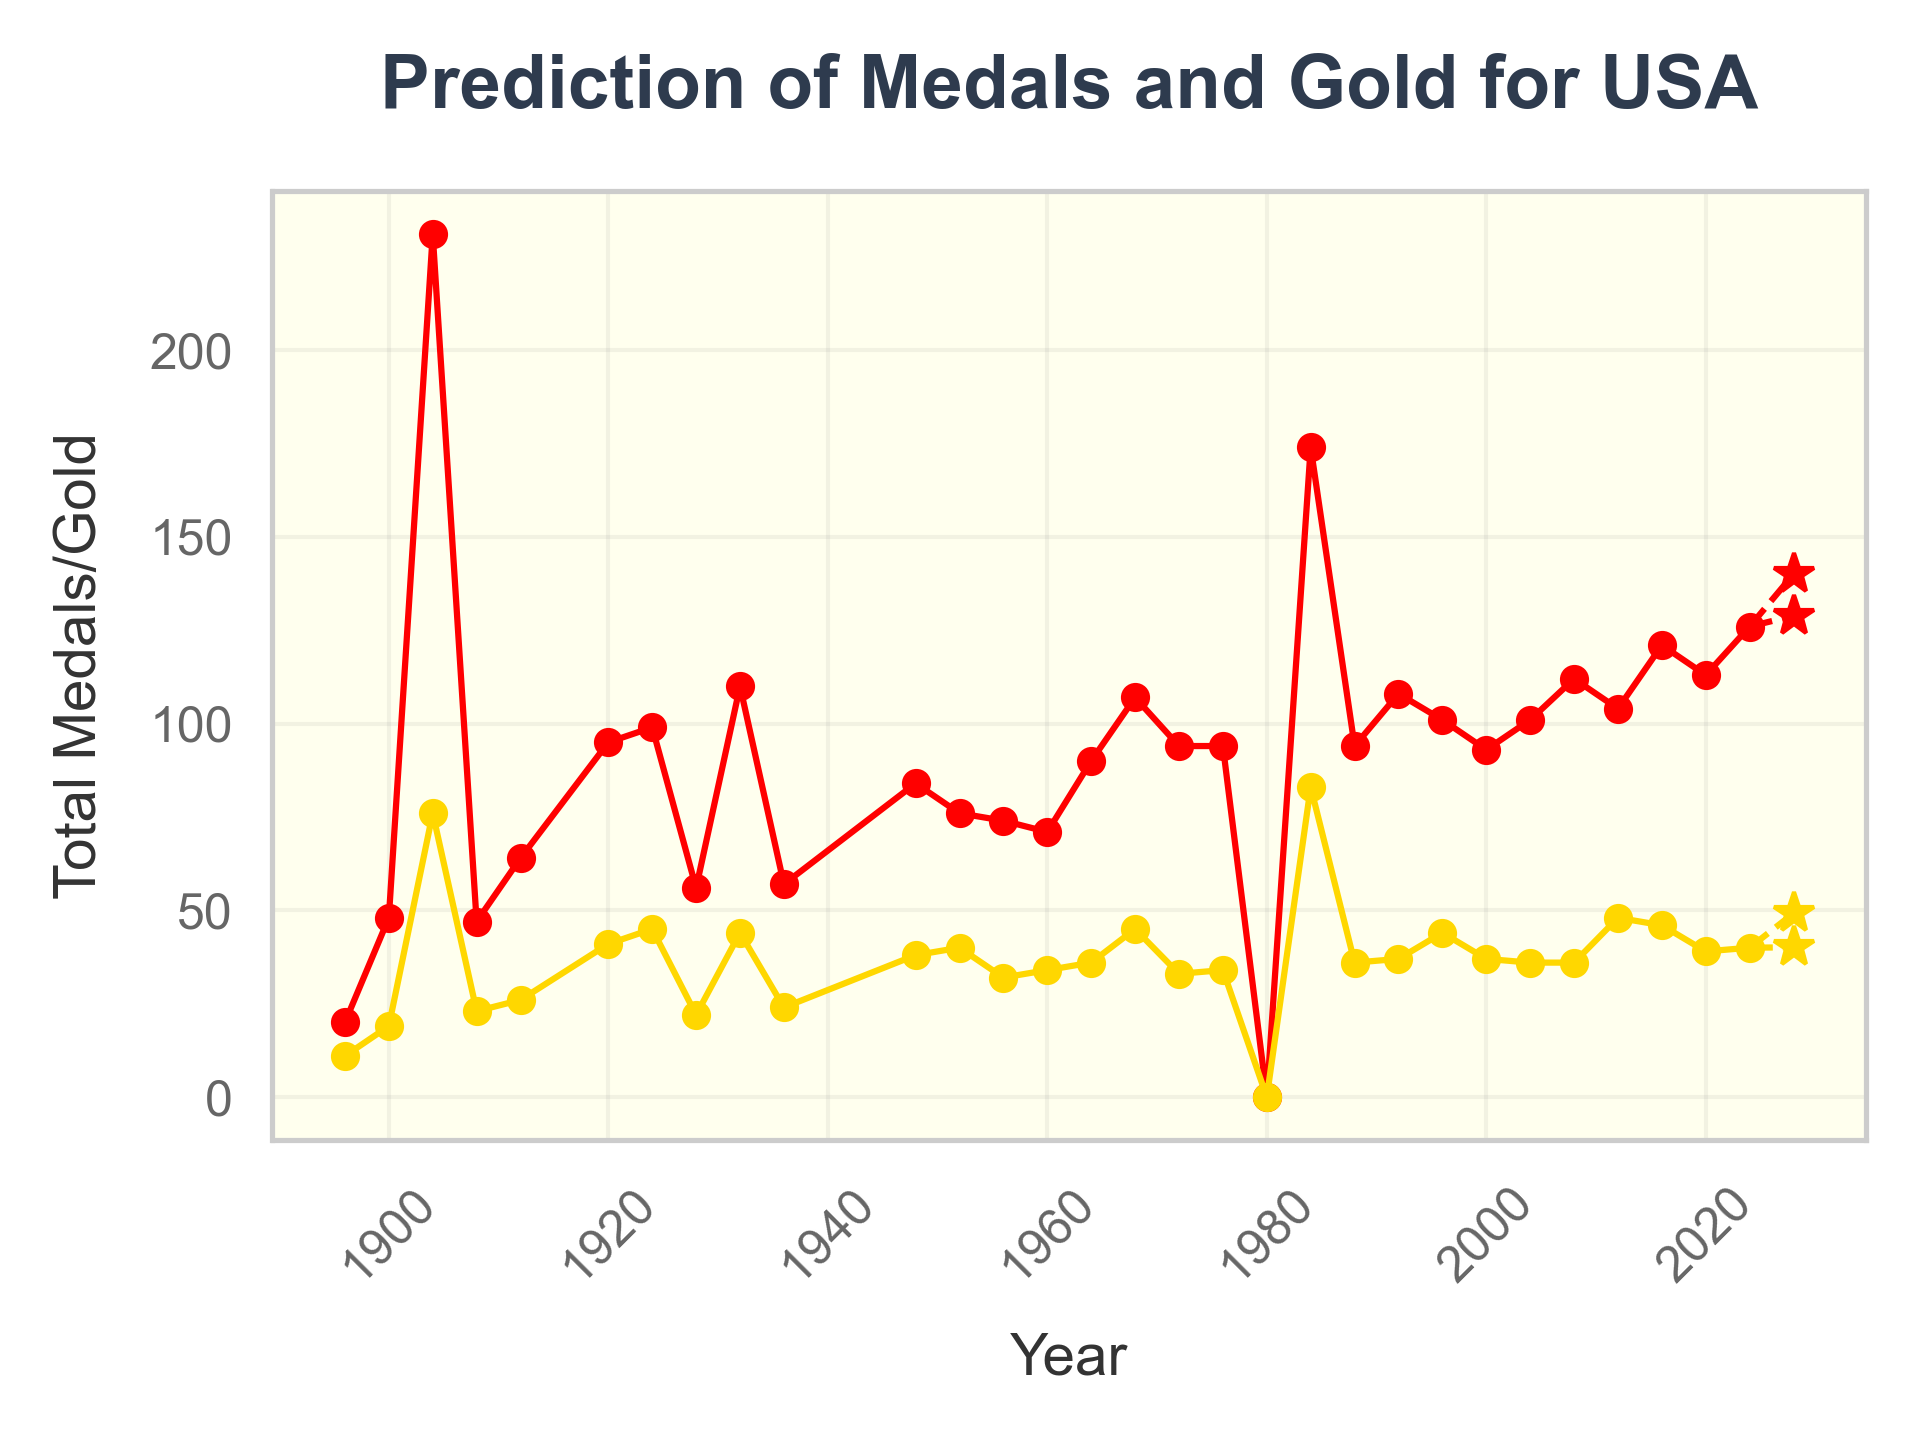
\includegraphics[width=0.45\linewidth]{predict/USA_medals_prediction.png}}
        \hfill % 水平填充
        \subfloat[]{\label{CHN}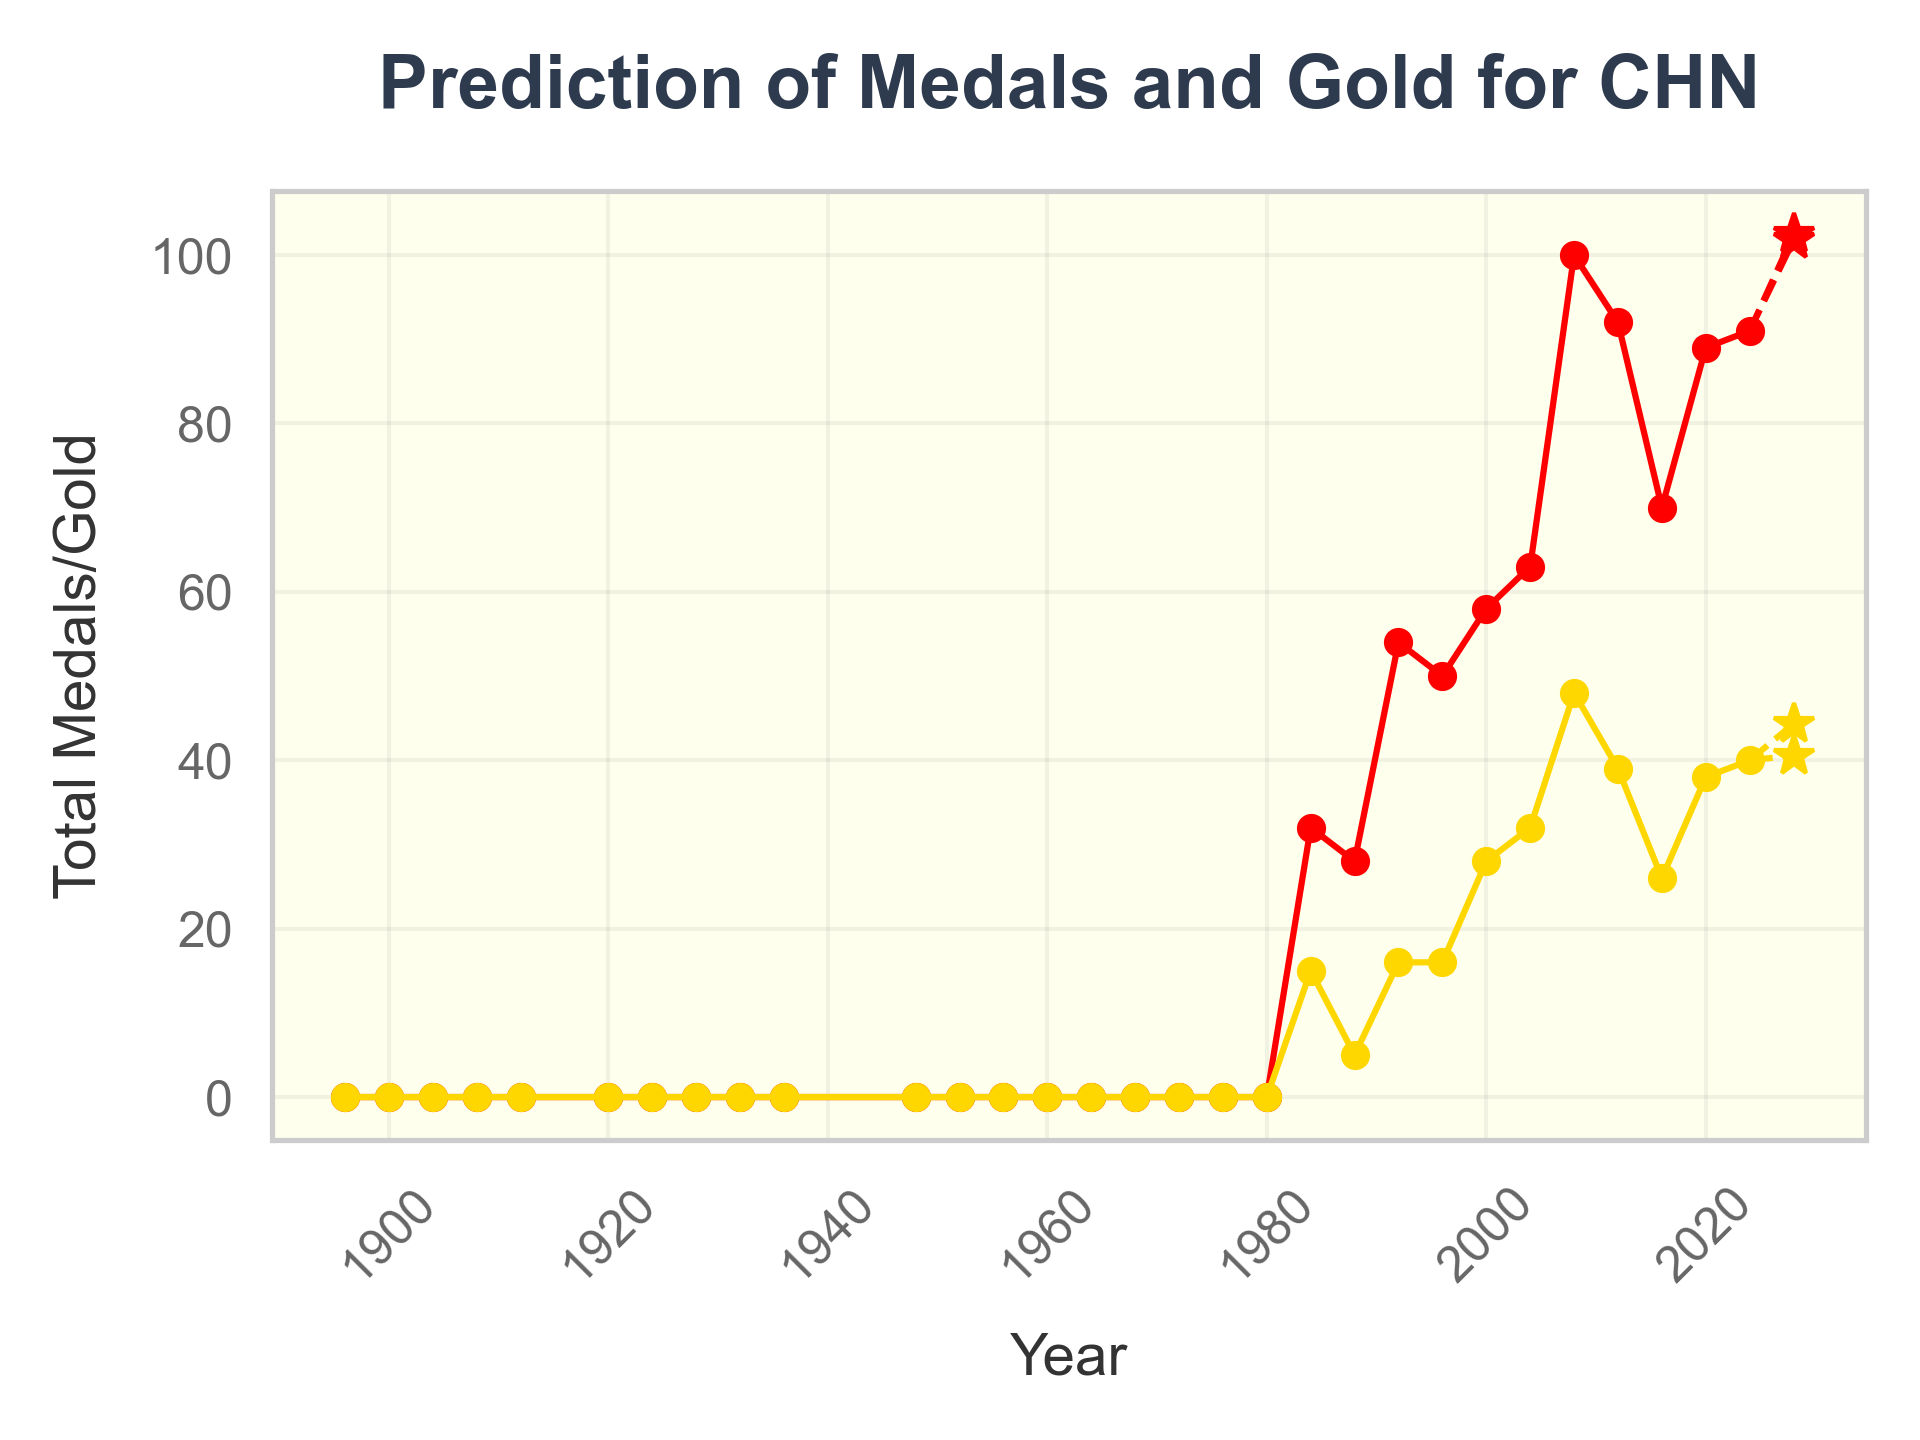
\includegraphics[width=0.45\linewidth]{predict/CHN_medals_prediction.png}}
    \end{minipage}
  
    
    % 第二行两张图片
    \begin{minipage}{1\linewidth}
        \subfloat[]{\label{FRA}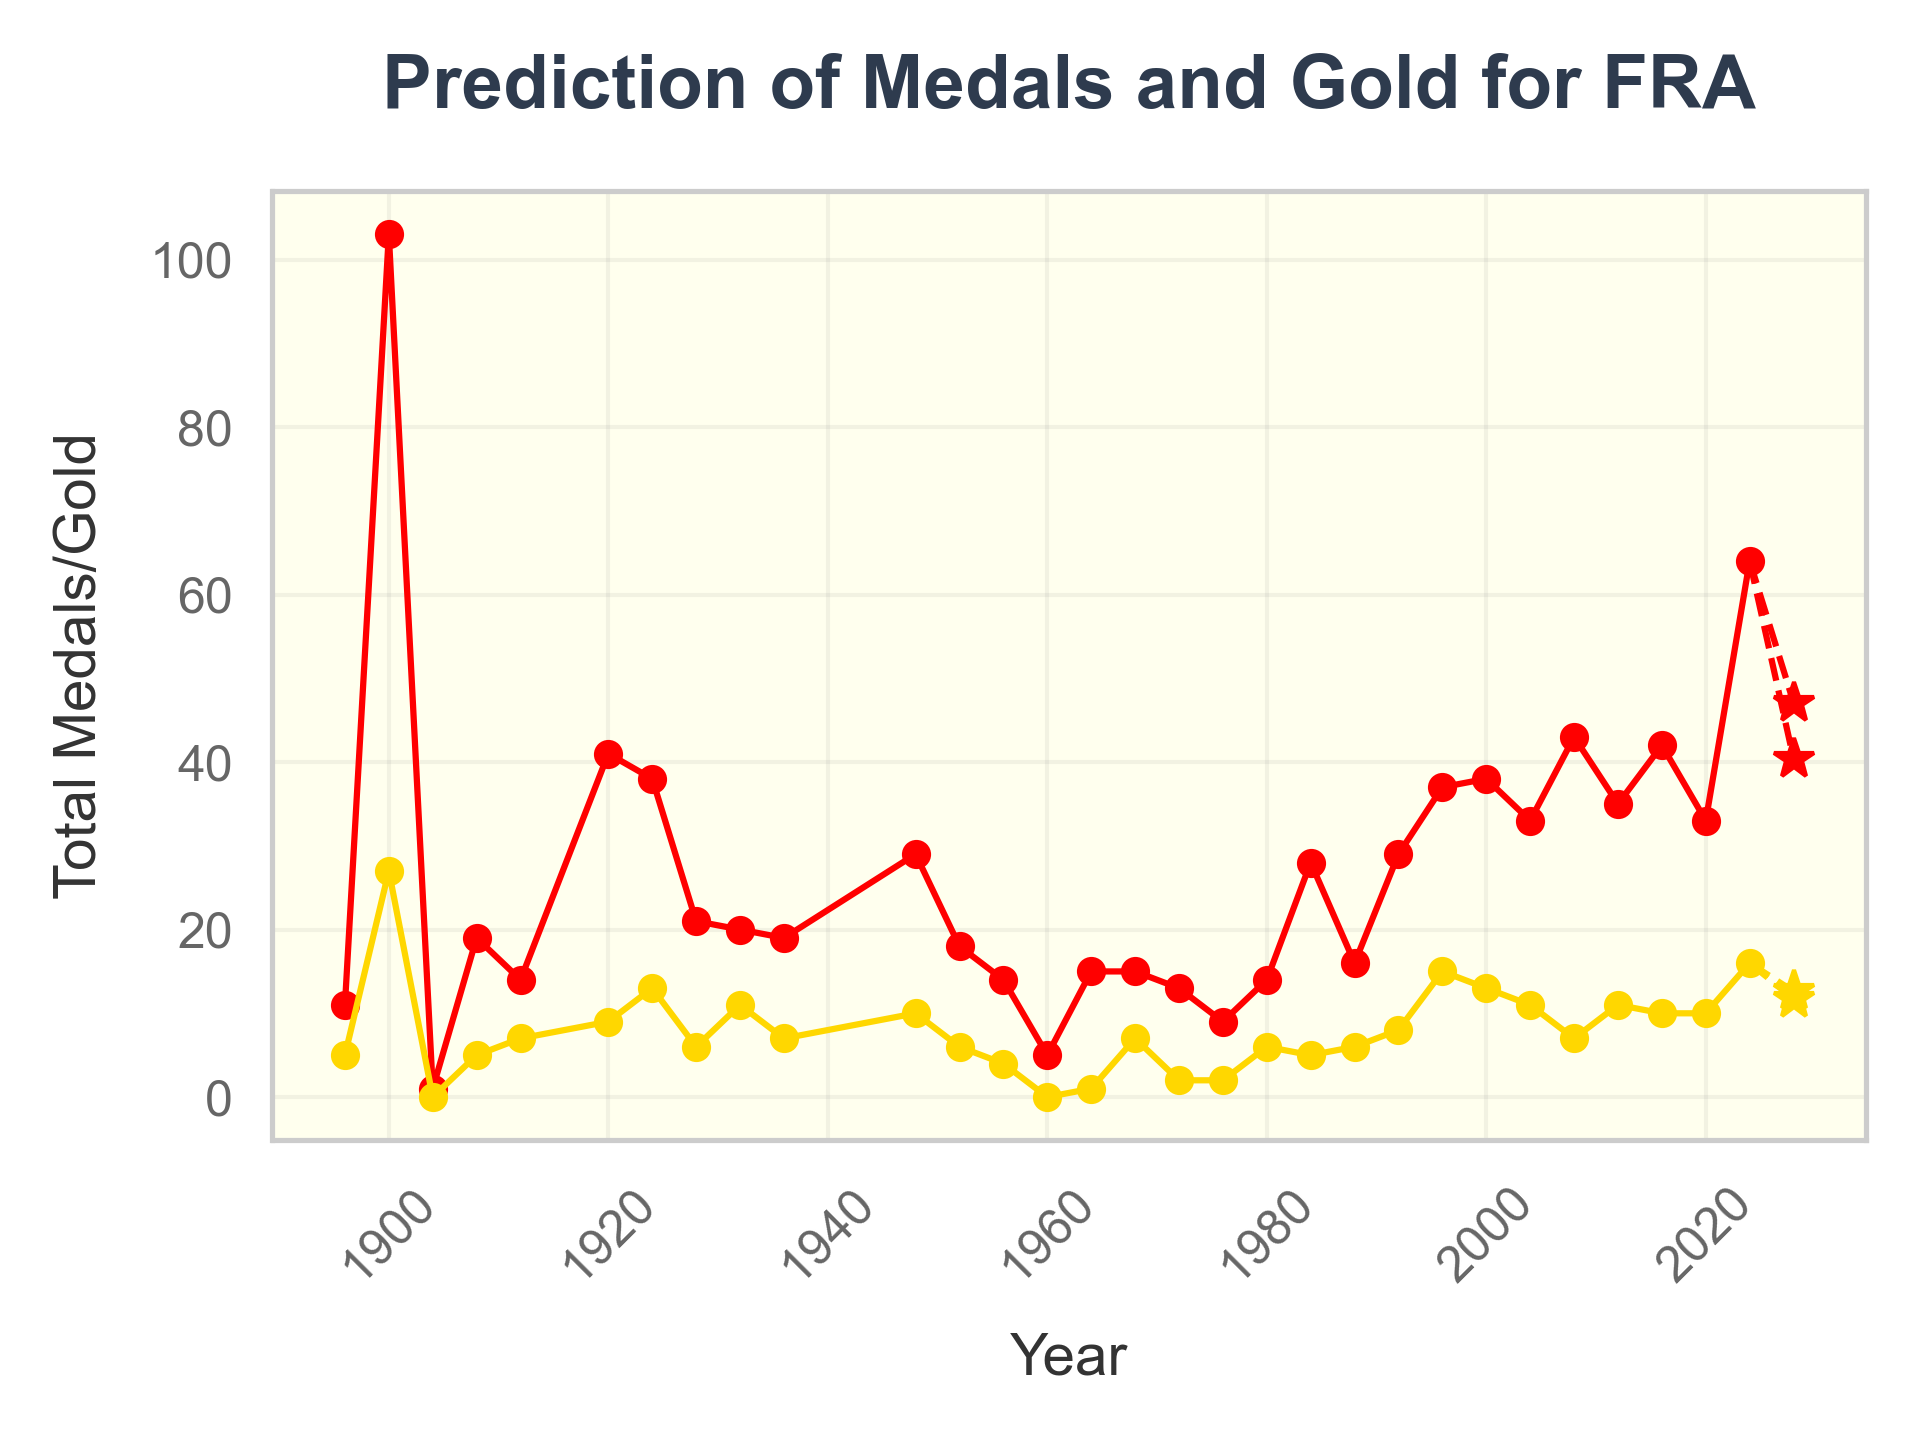
\includegraphics[width=0.45\linewidth]{predict/FRA_medals_prediction.png}}
        \hfill % 水平填充
        \subfloat[]{\label{GRE}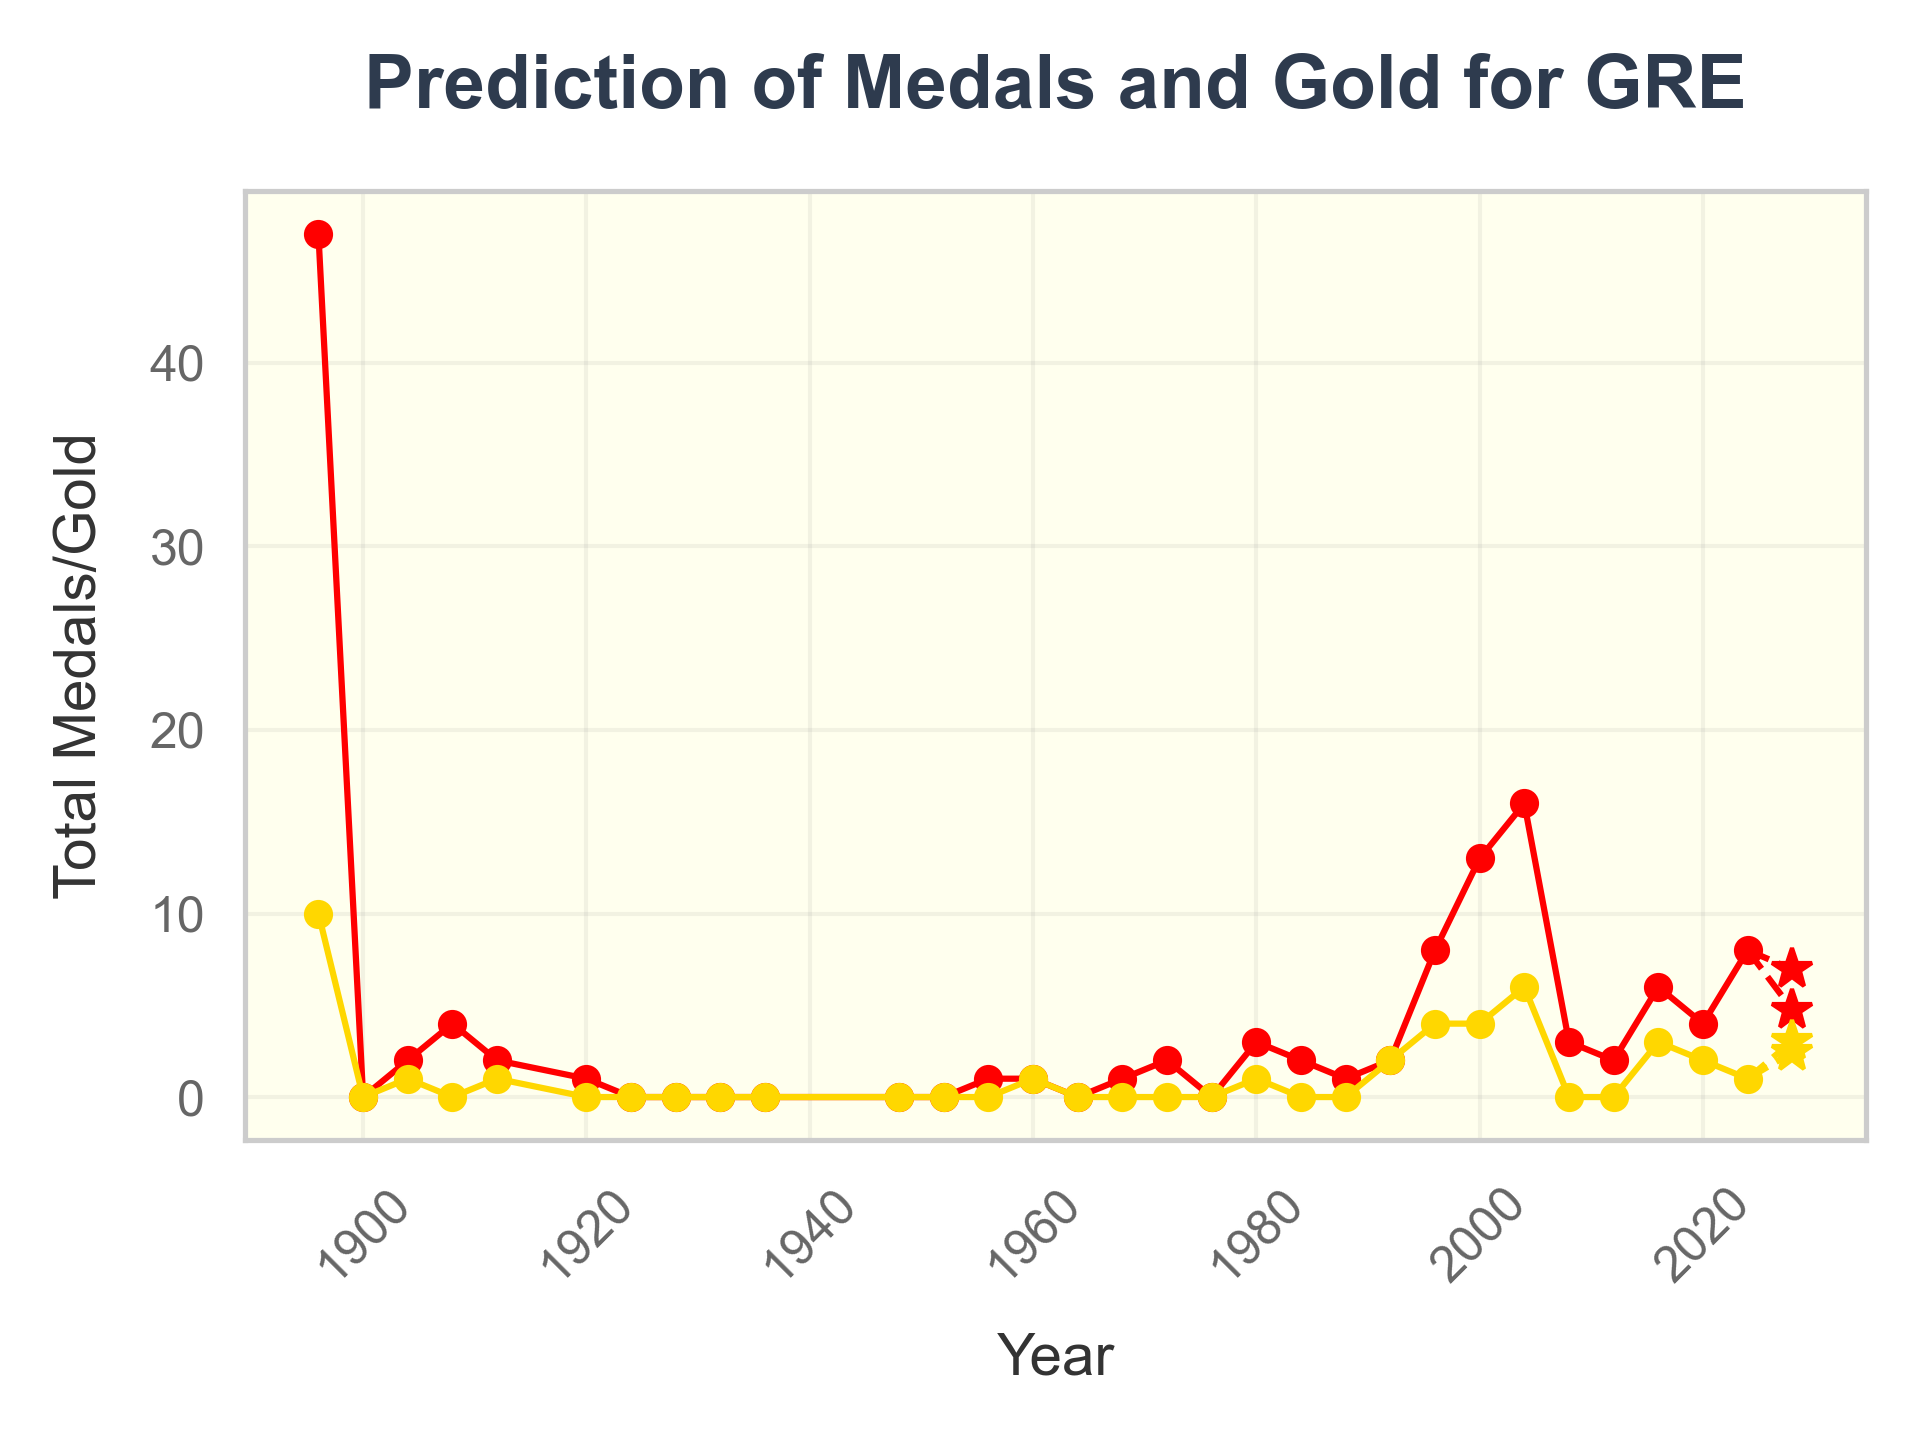
\includegraphics[width=0.45\linewidth]{predict/GRE_medals_prediction.png}}
    \end{minipage}

    
    % 第三行两张图片
    \begin{minipage}{1\linewidth}
        \subfloat[]{\label{INA}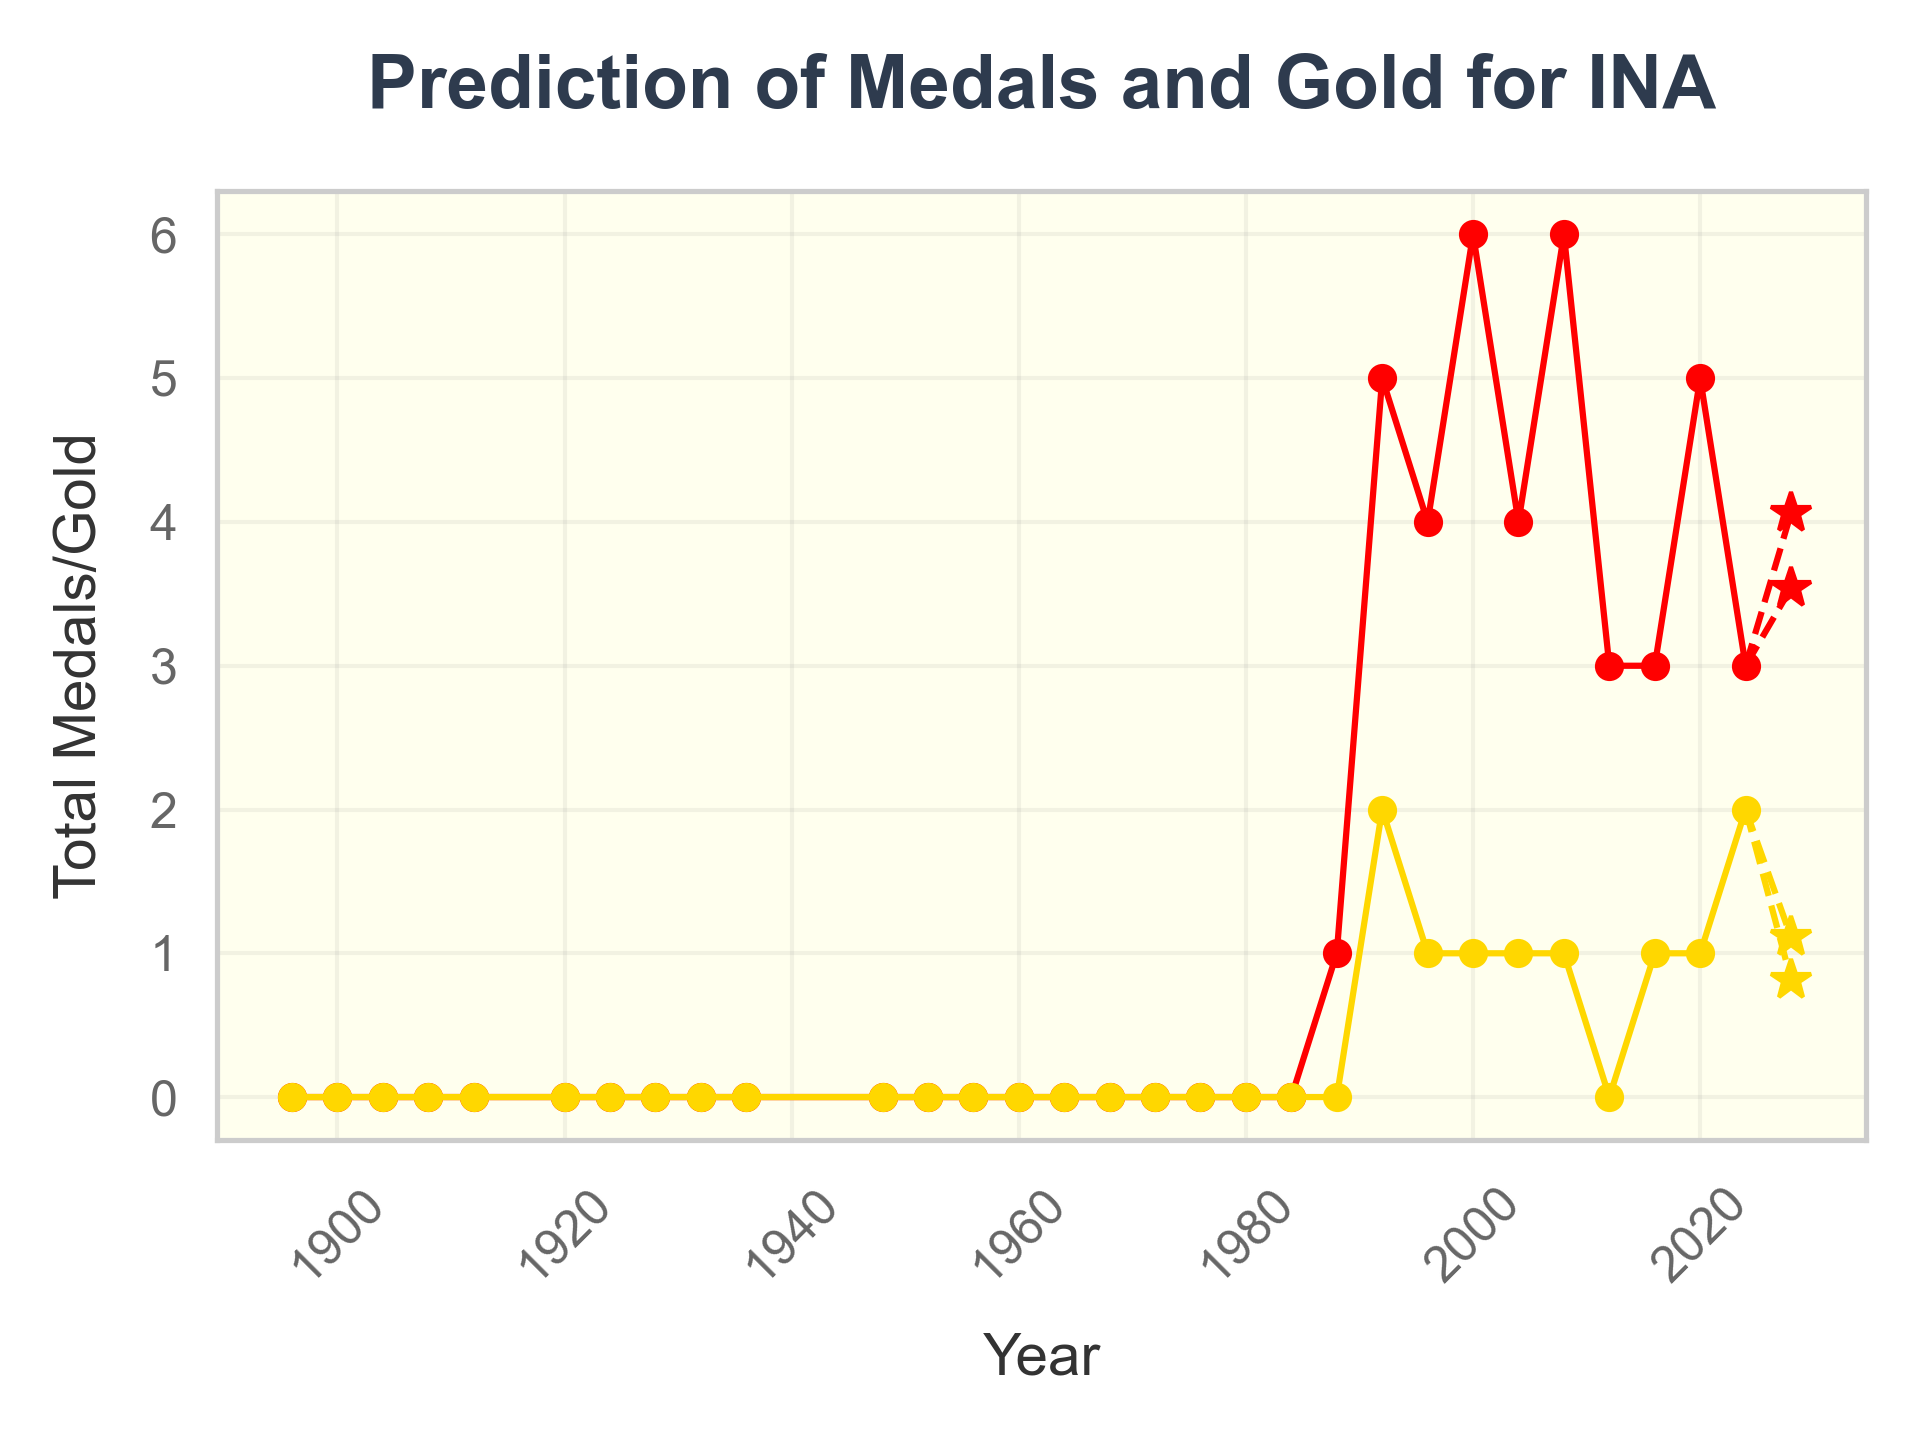
\includegraphics[width=0.45\linewidth]{predict/INA_medals_prediction.png}}
        \hfill % 水平填充
        \subfloat[]{\label{TPE}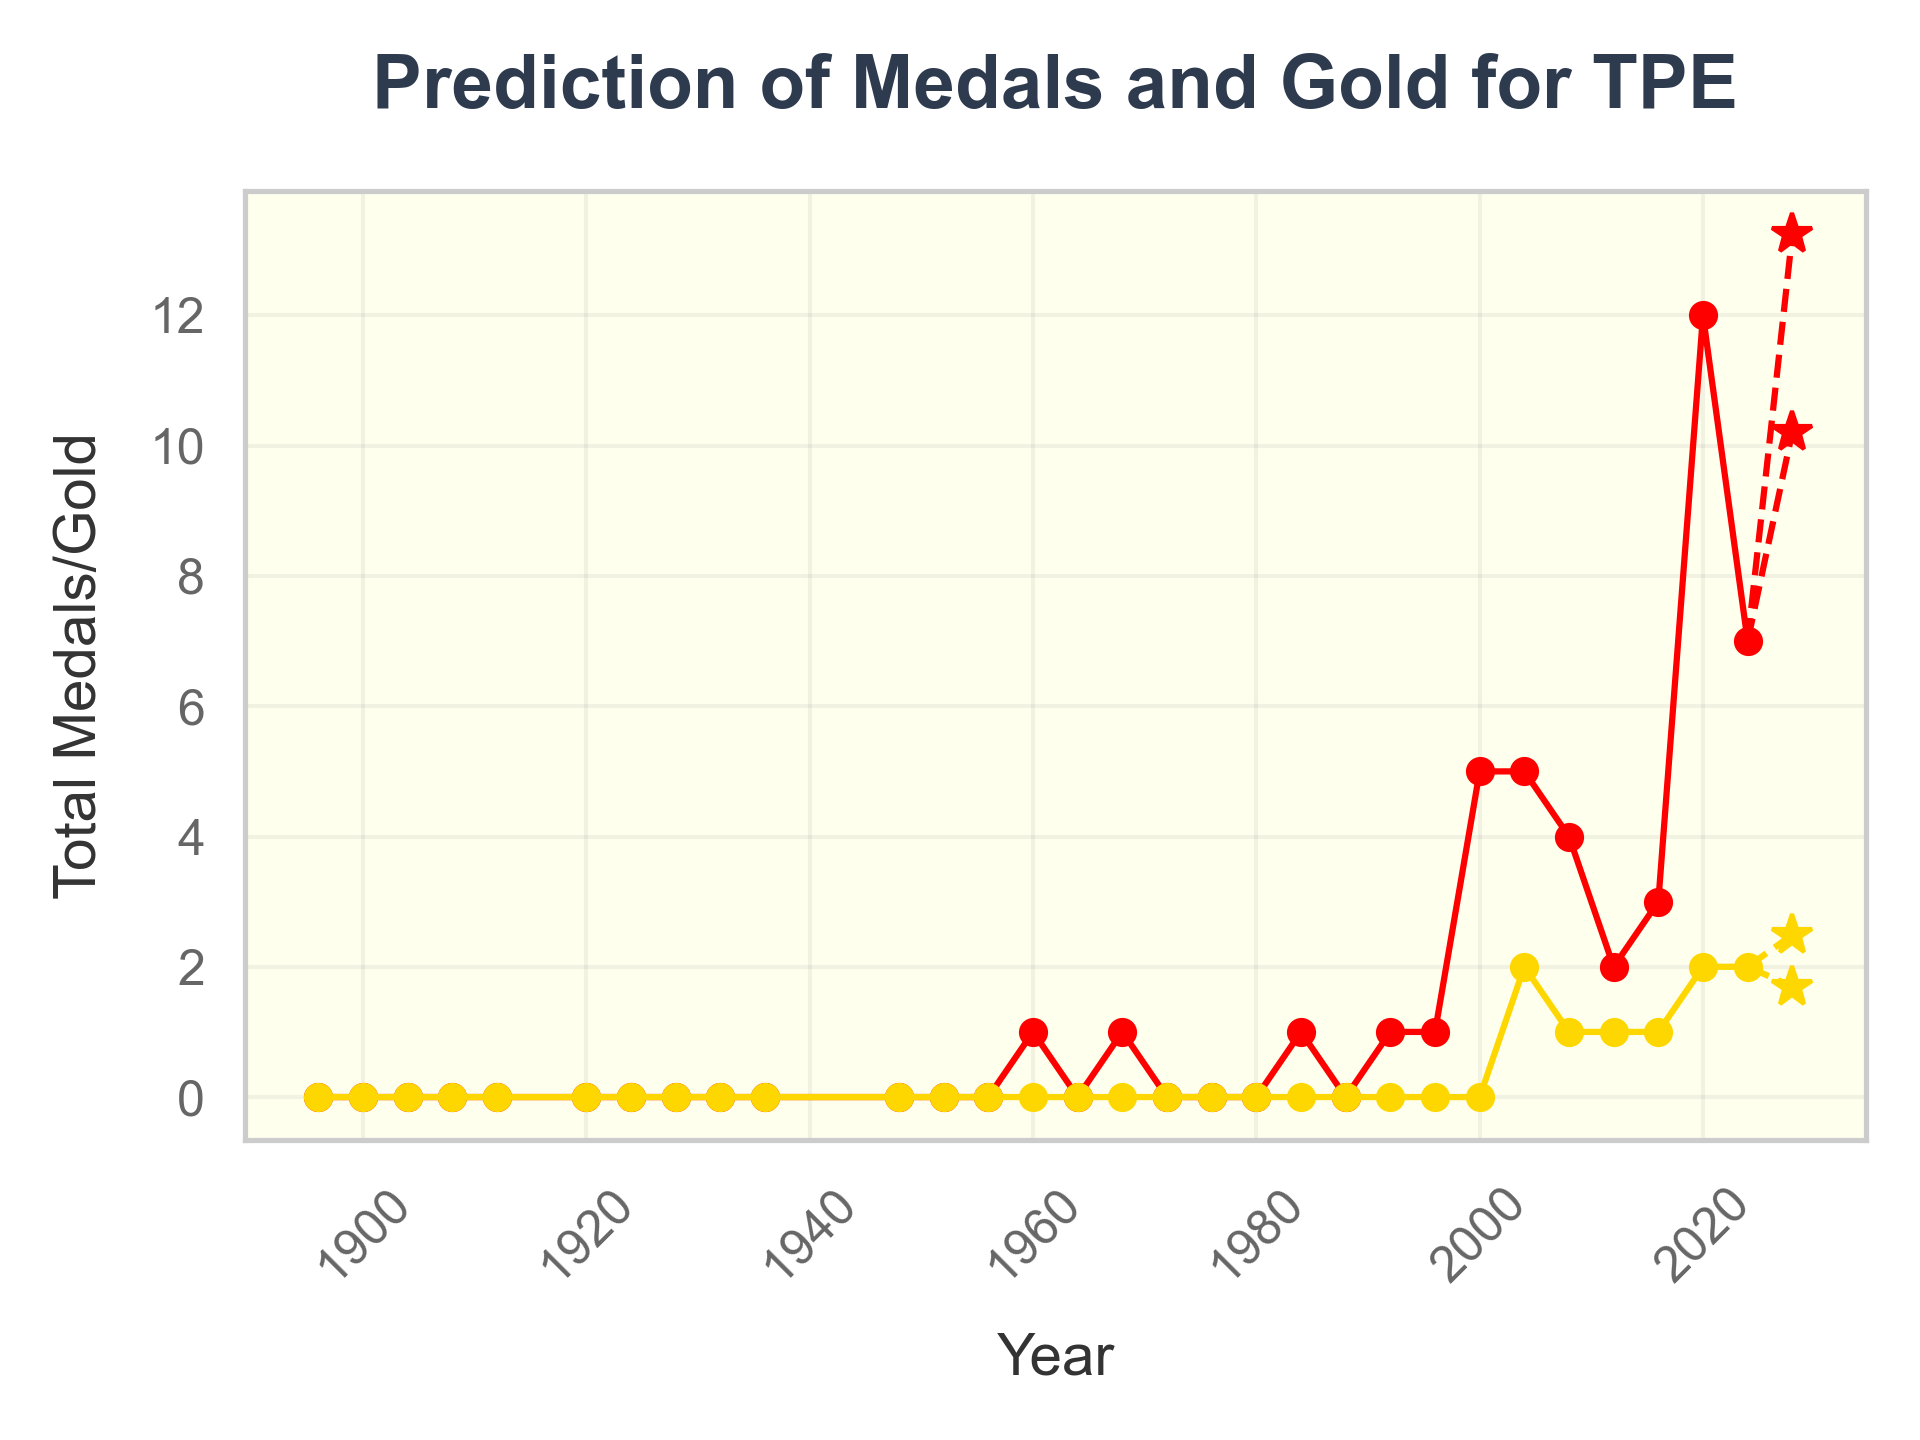
\includegraphics[width=0.45\linewidth]{predict/TPE_medals_prediction.png}}
    \end{minipage}
    
    \caption{Prediction Intervals for Total Medals and Gold Medals of Different Countries} \label{fig:8-11}
\end{figure}

Using the trained model, predictions were made for the three categories of countries. The normalized prediction results were denormalized back to their original values, and the results are shown in Figure 8. Green indicates an increase in medals, red indicates a decrease, and blue indicates a stable trend. The bar chart represents a range of values.

\begin{figure}[H]
	\centering
	\subfloat[Category 1] {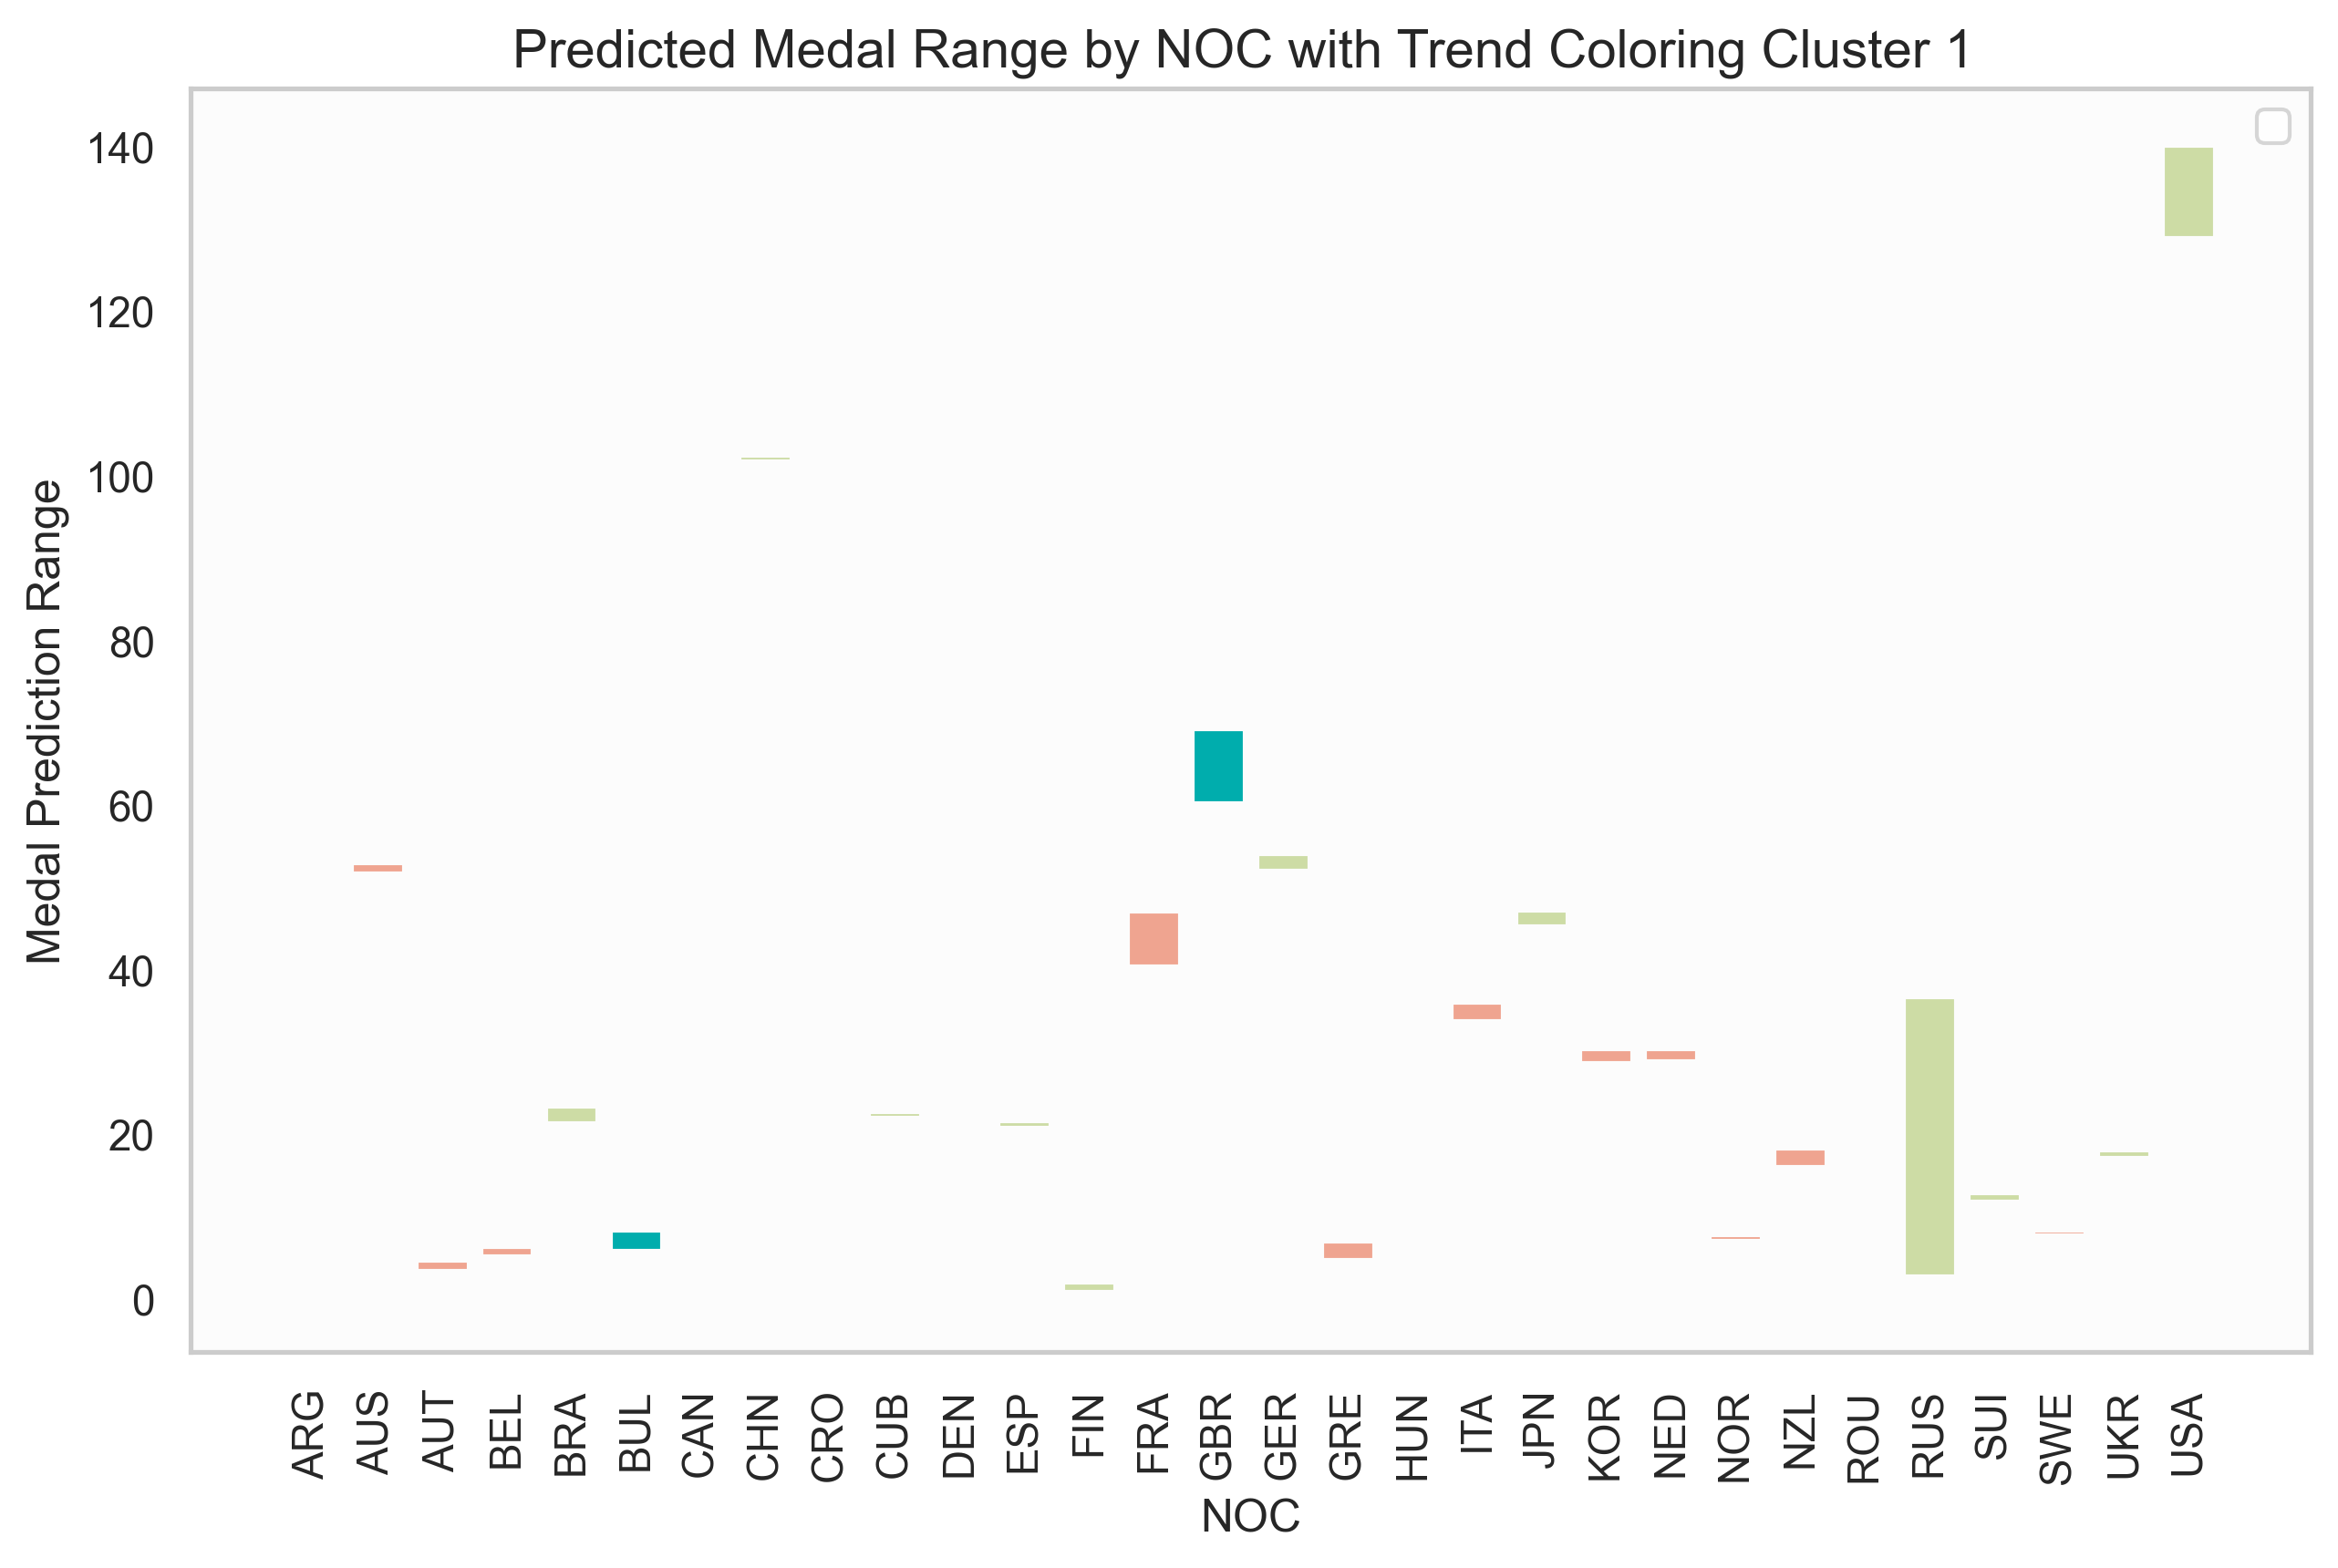
\includegraphics[width=.3\textwidth]{graph/res1.png}}
	\subfloat[Category 2] {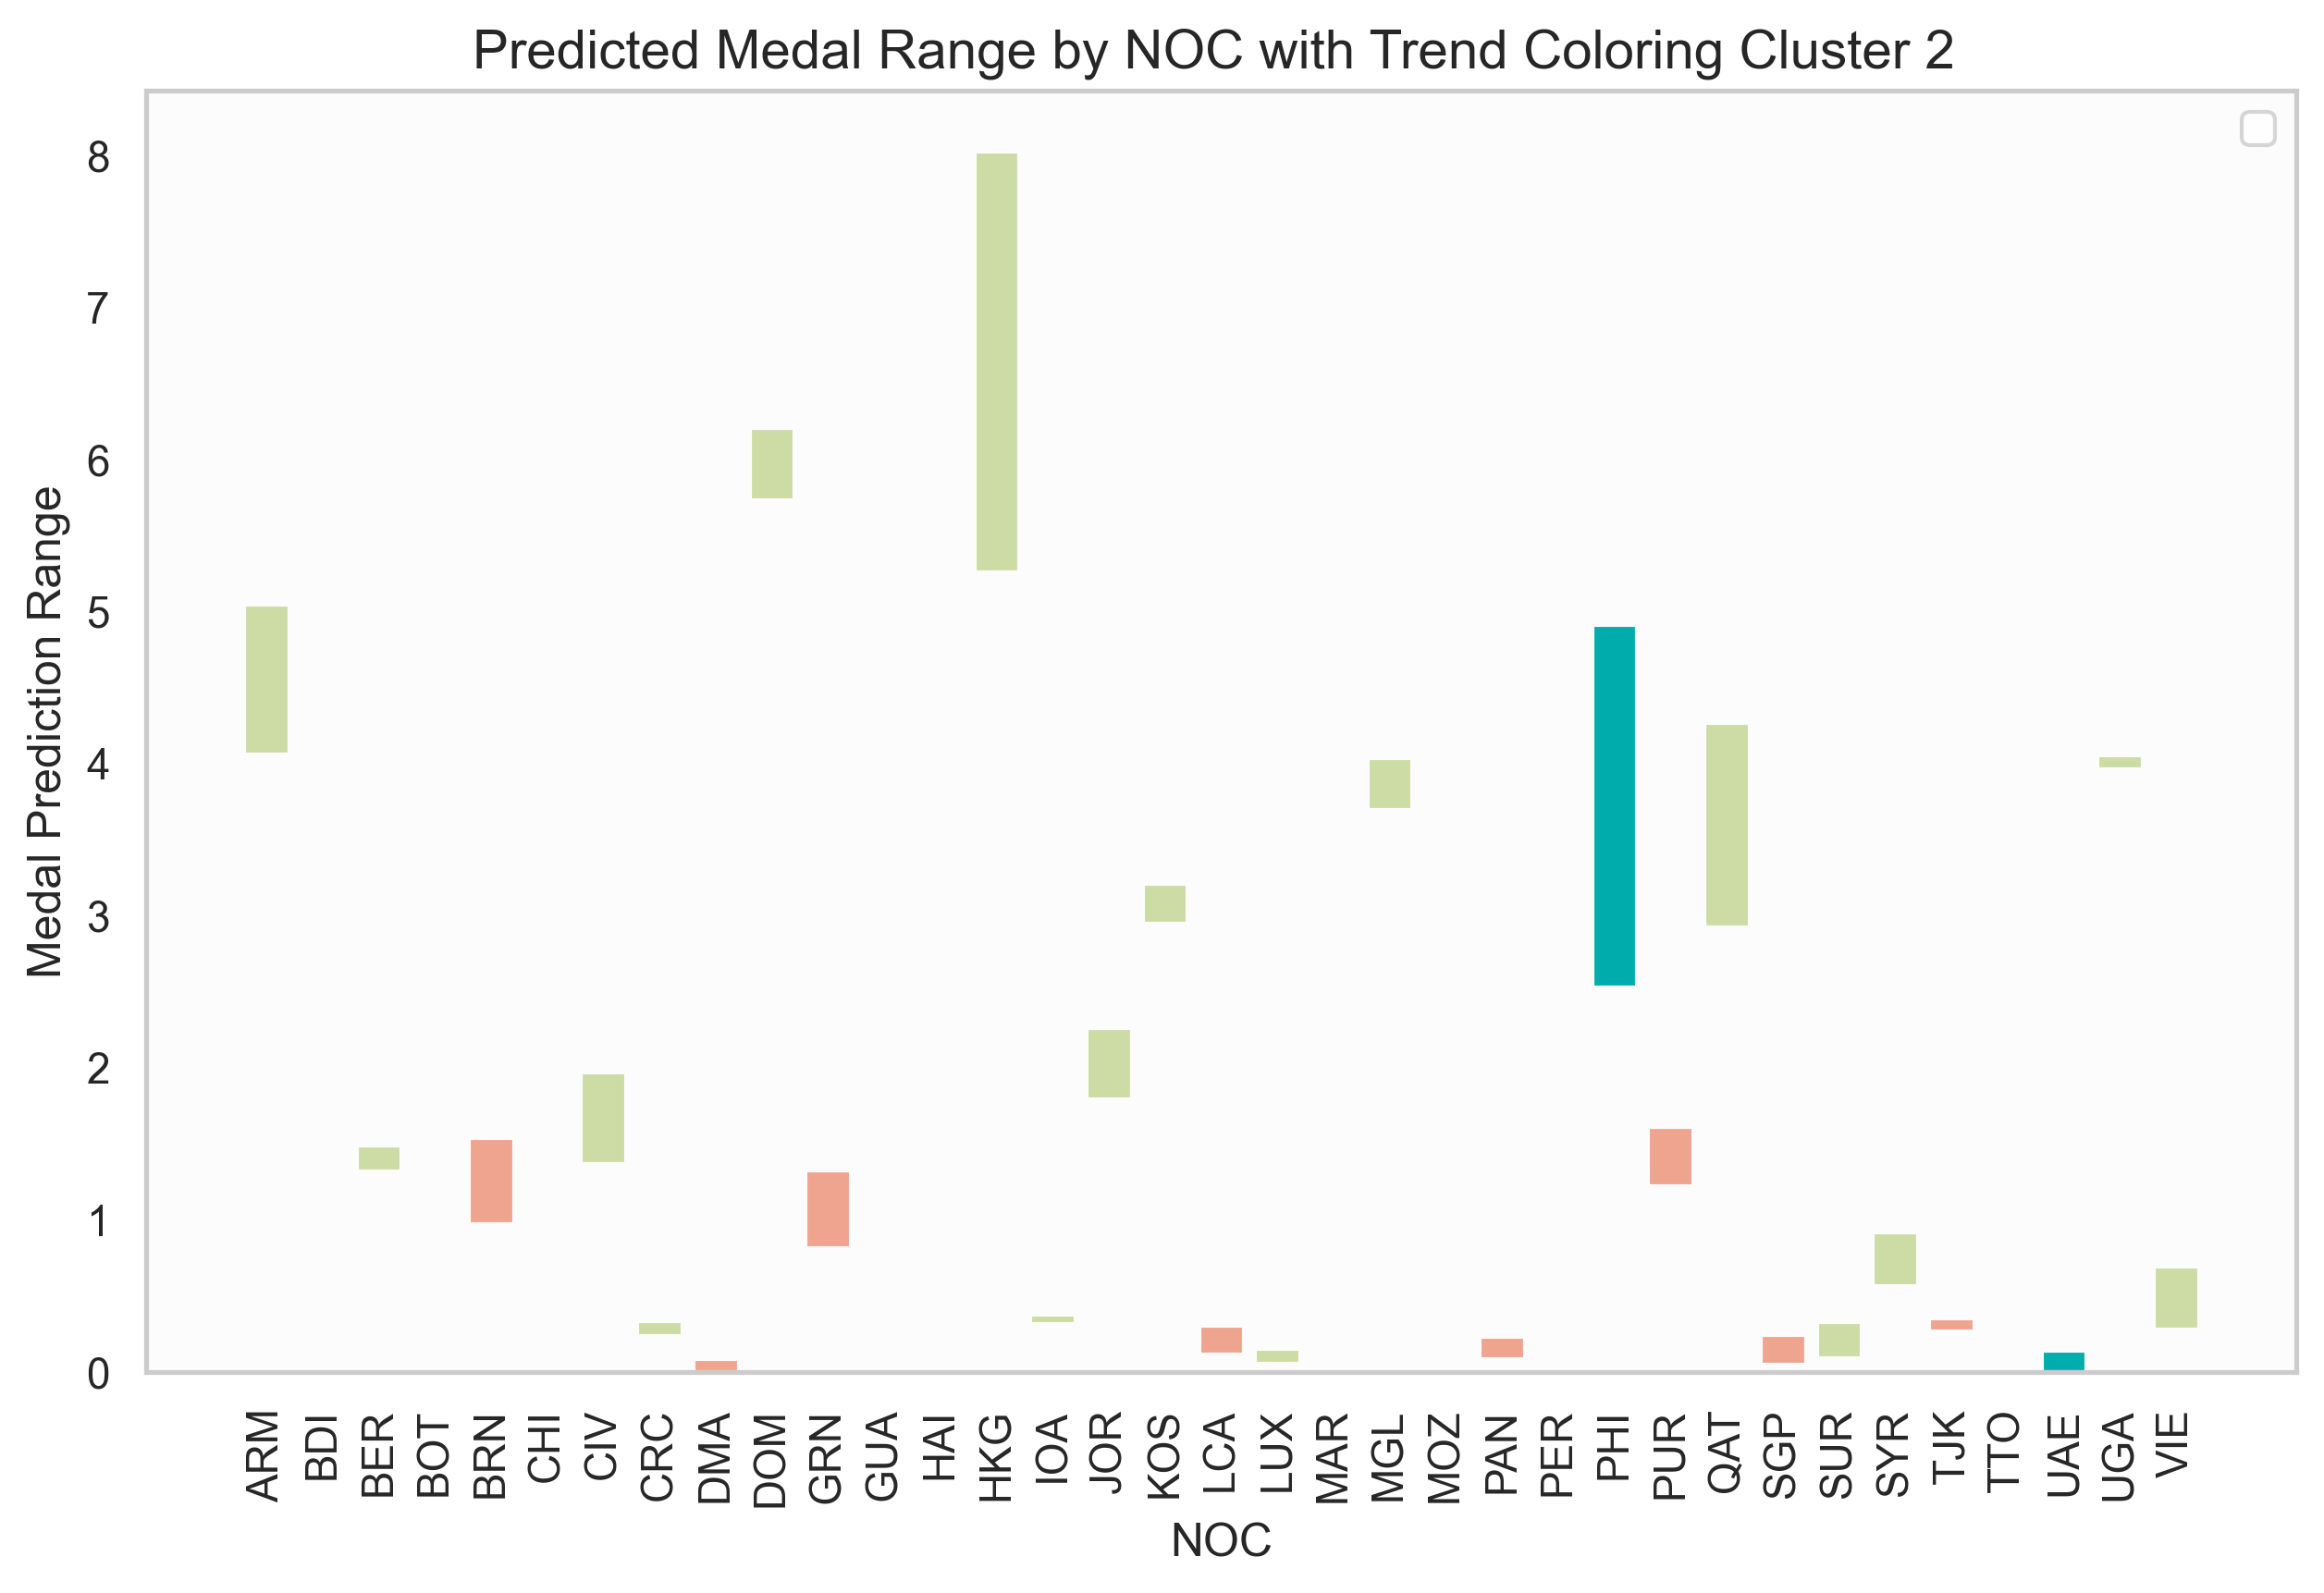
\includegraphics[width=.3\textwidth]{graph/res2.png}}
	\subfloat[Category 3] {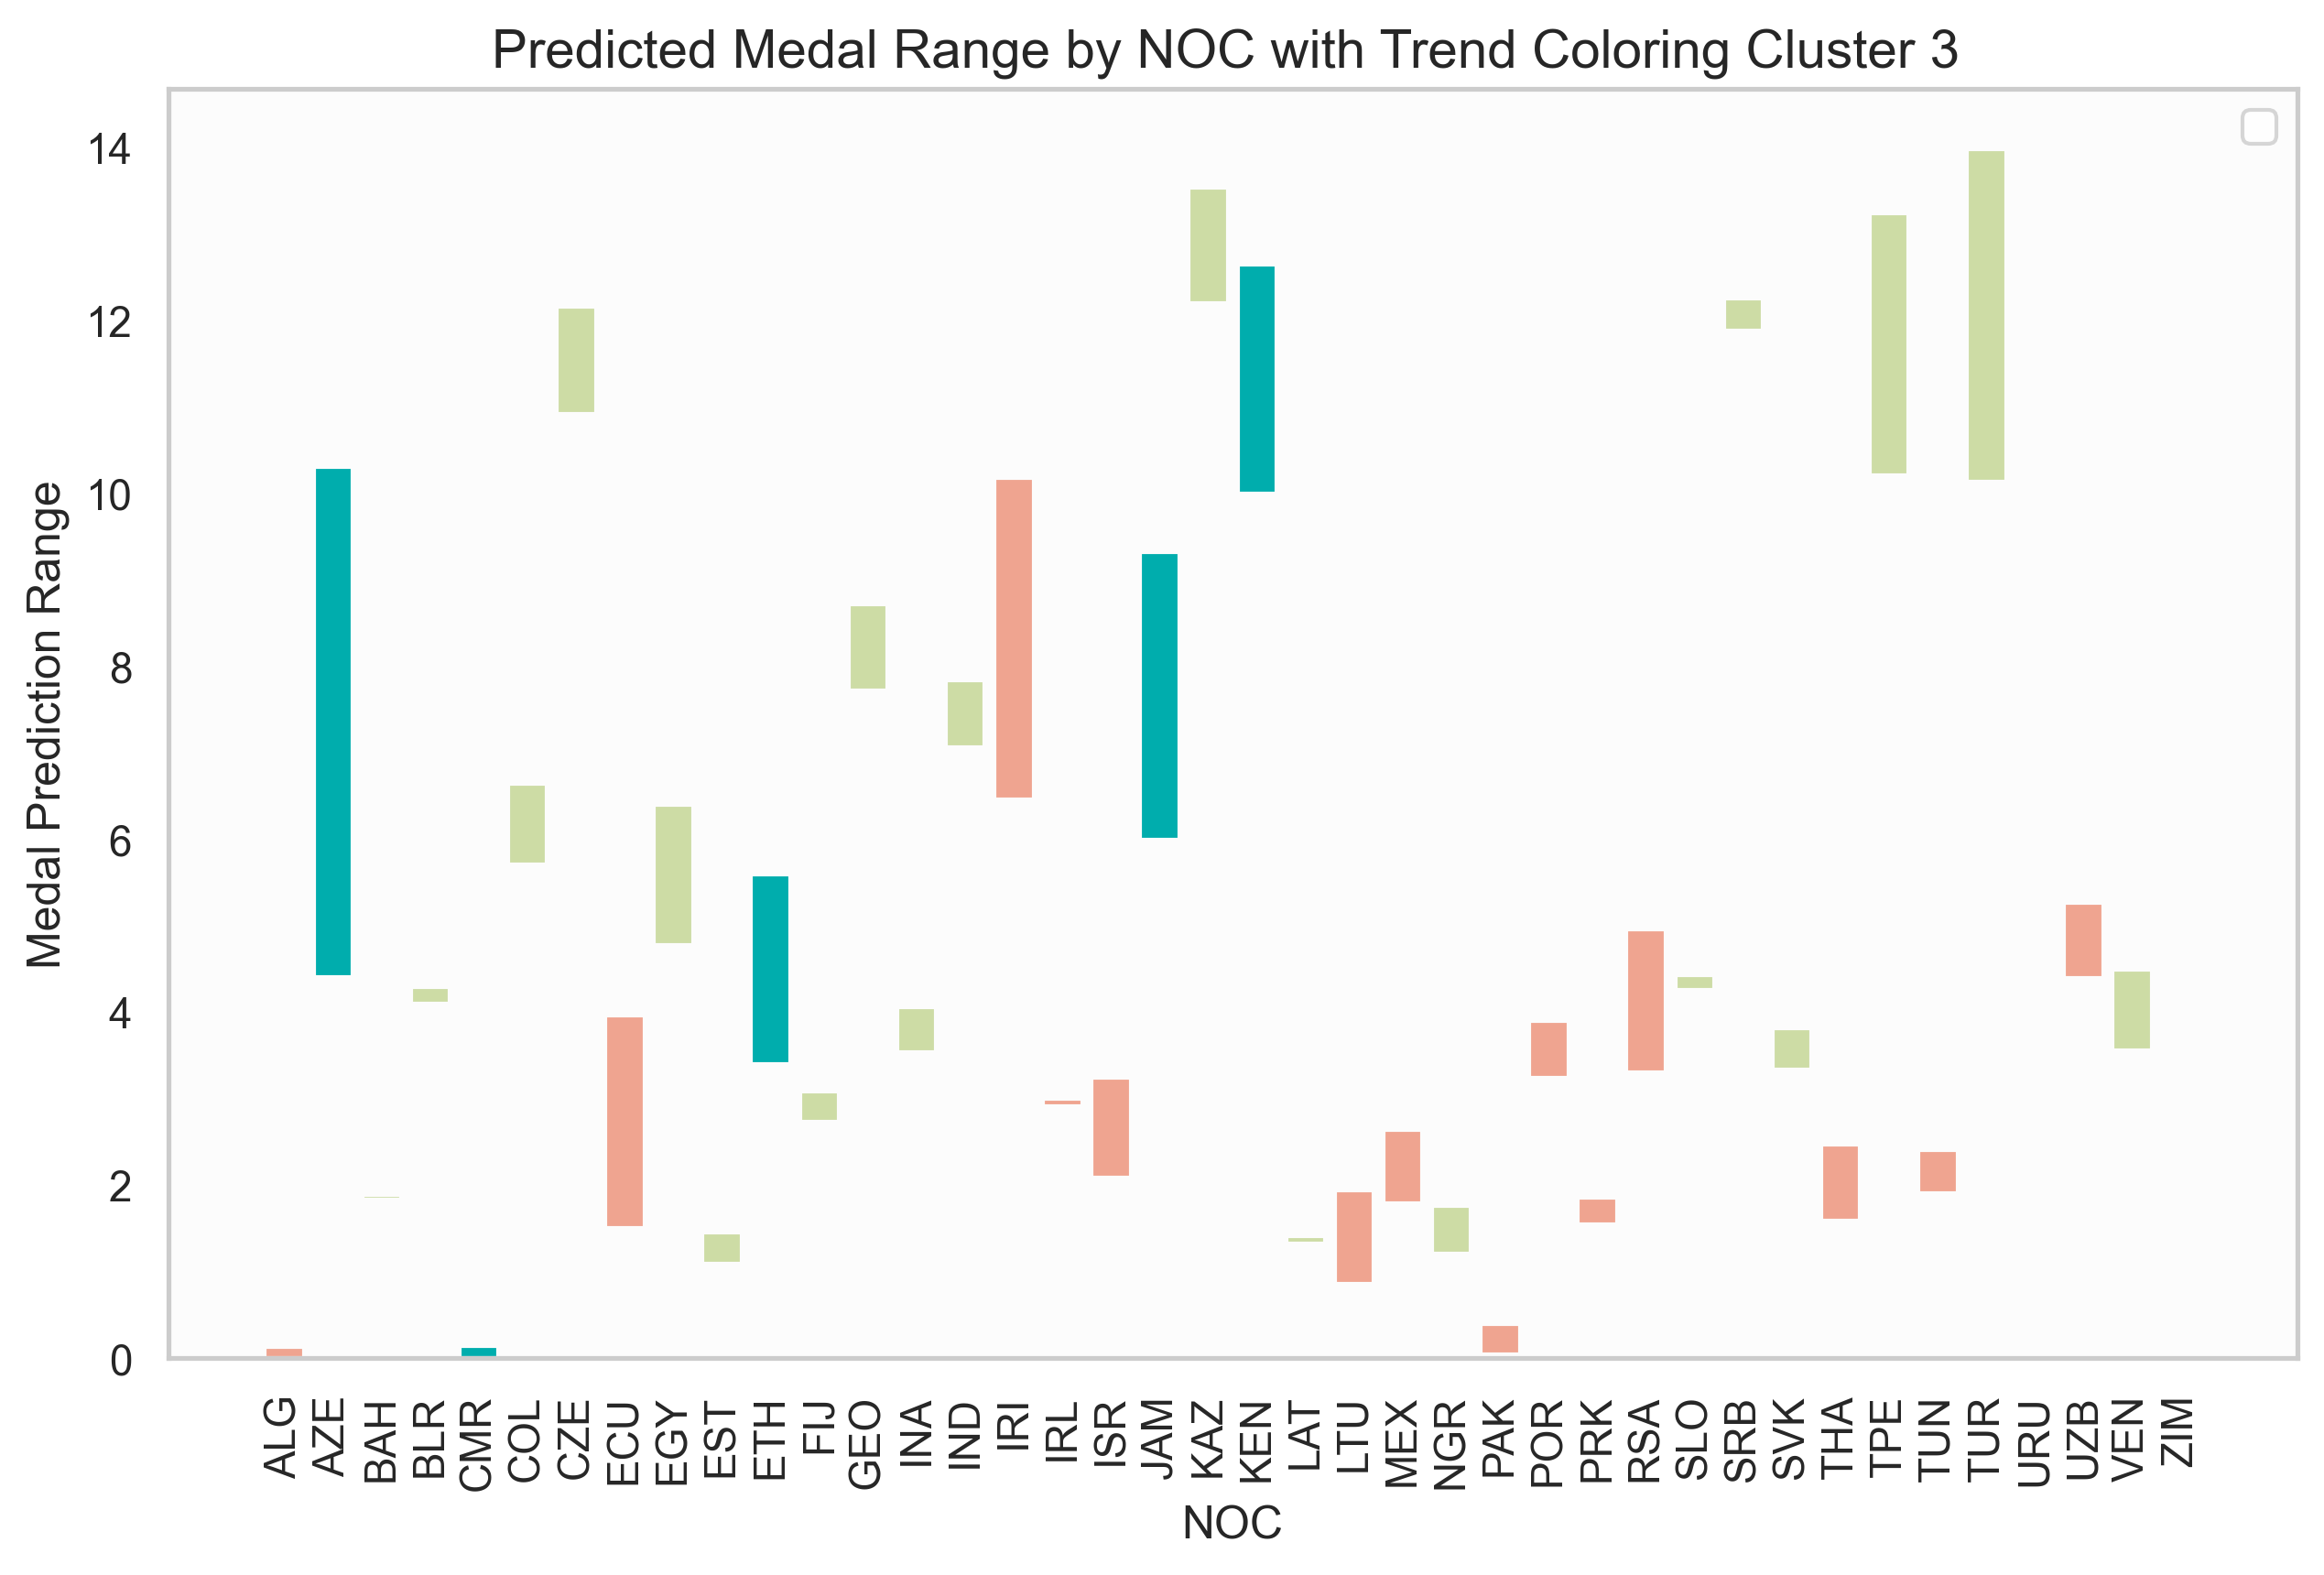
\includegraphics[width=.3\textwidth]{graph/res3.png}}
	\caption{Total Medal Predictions for Category 3 Countries}
	\label{fig_E1}
\end{figure}

\begin{figure}[H]
	\centering
	\subfloat[Category 1] {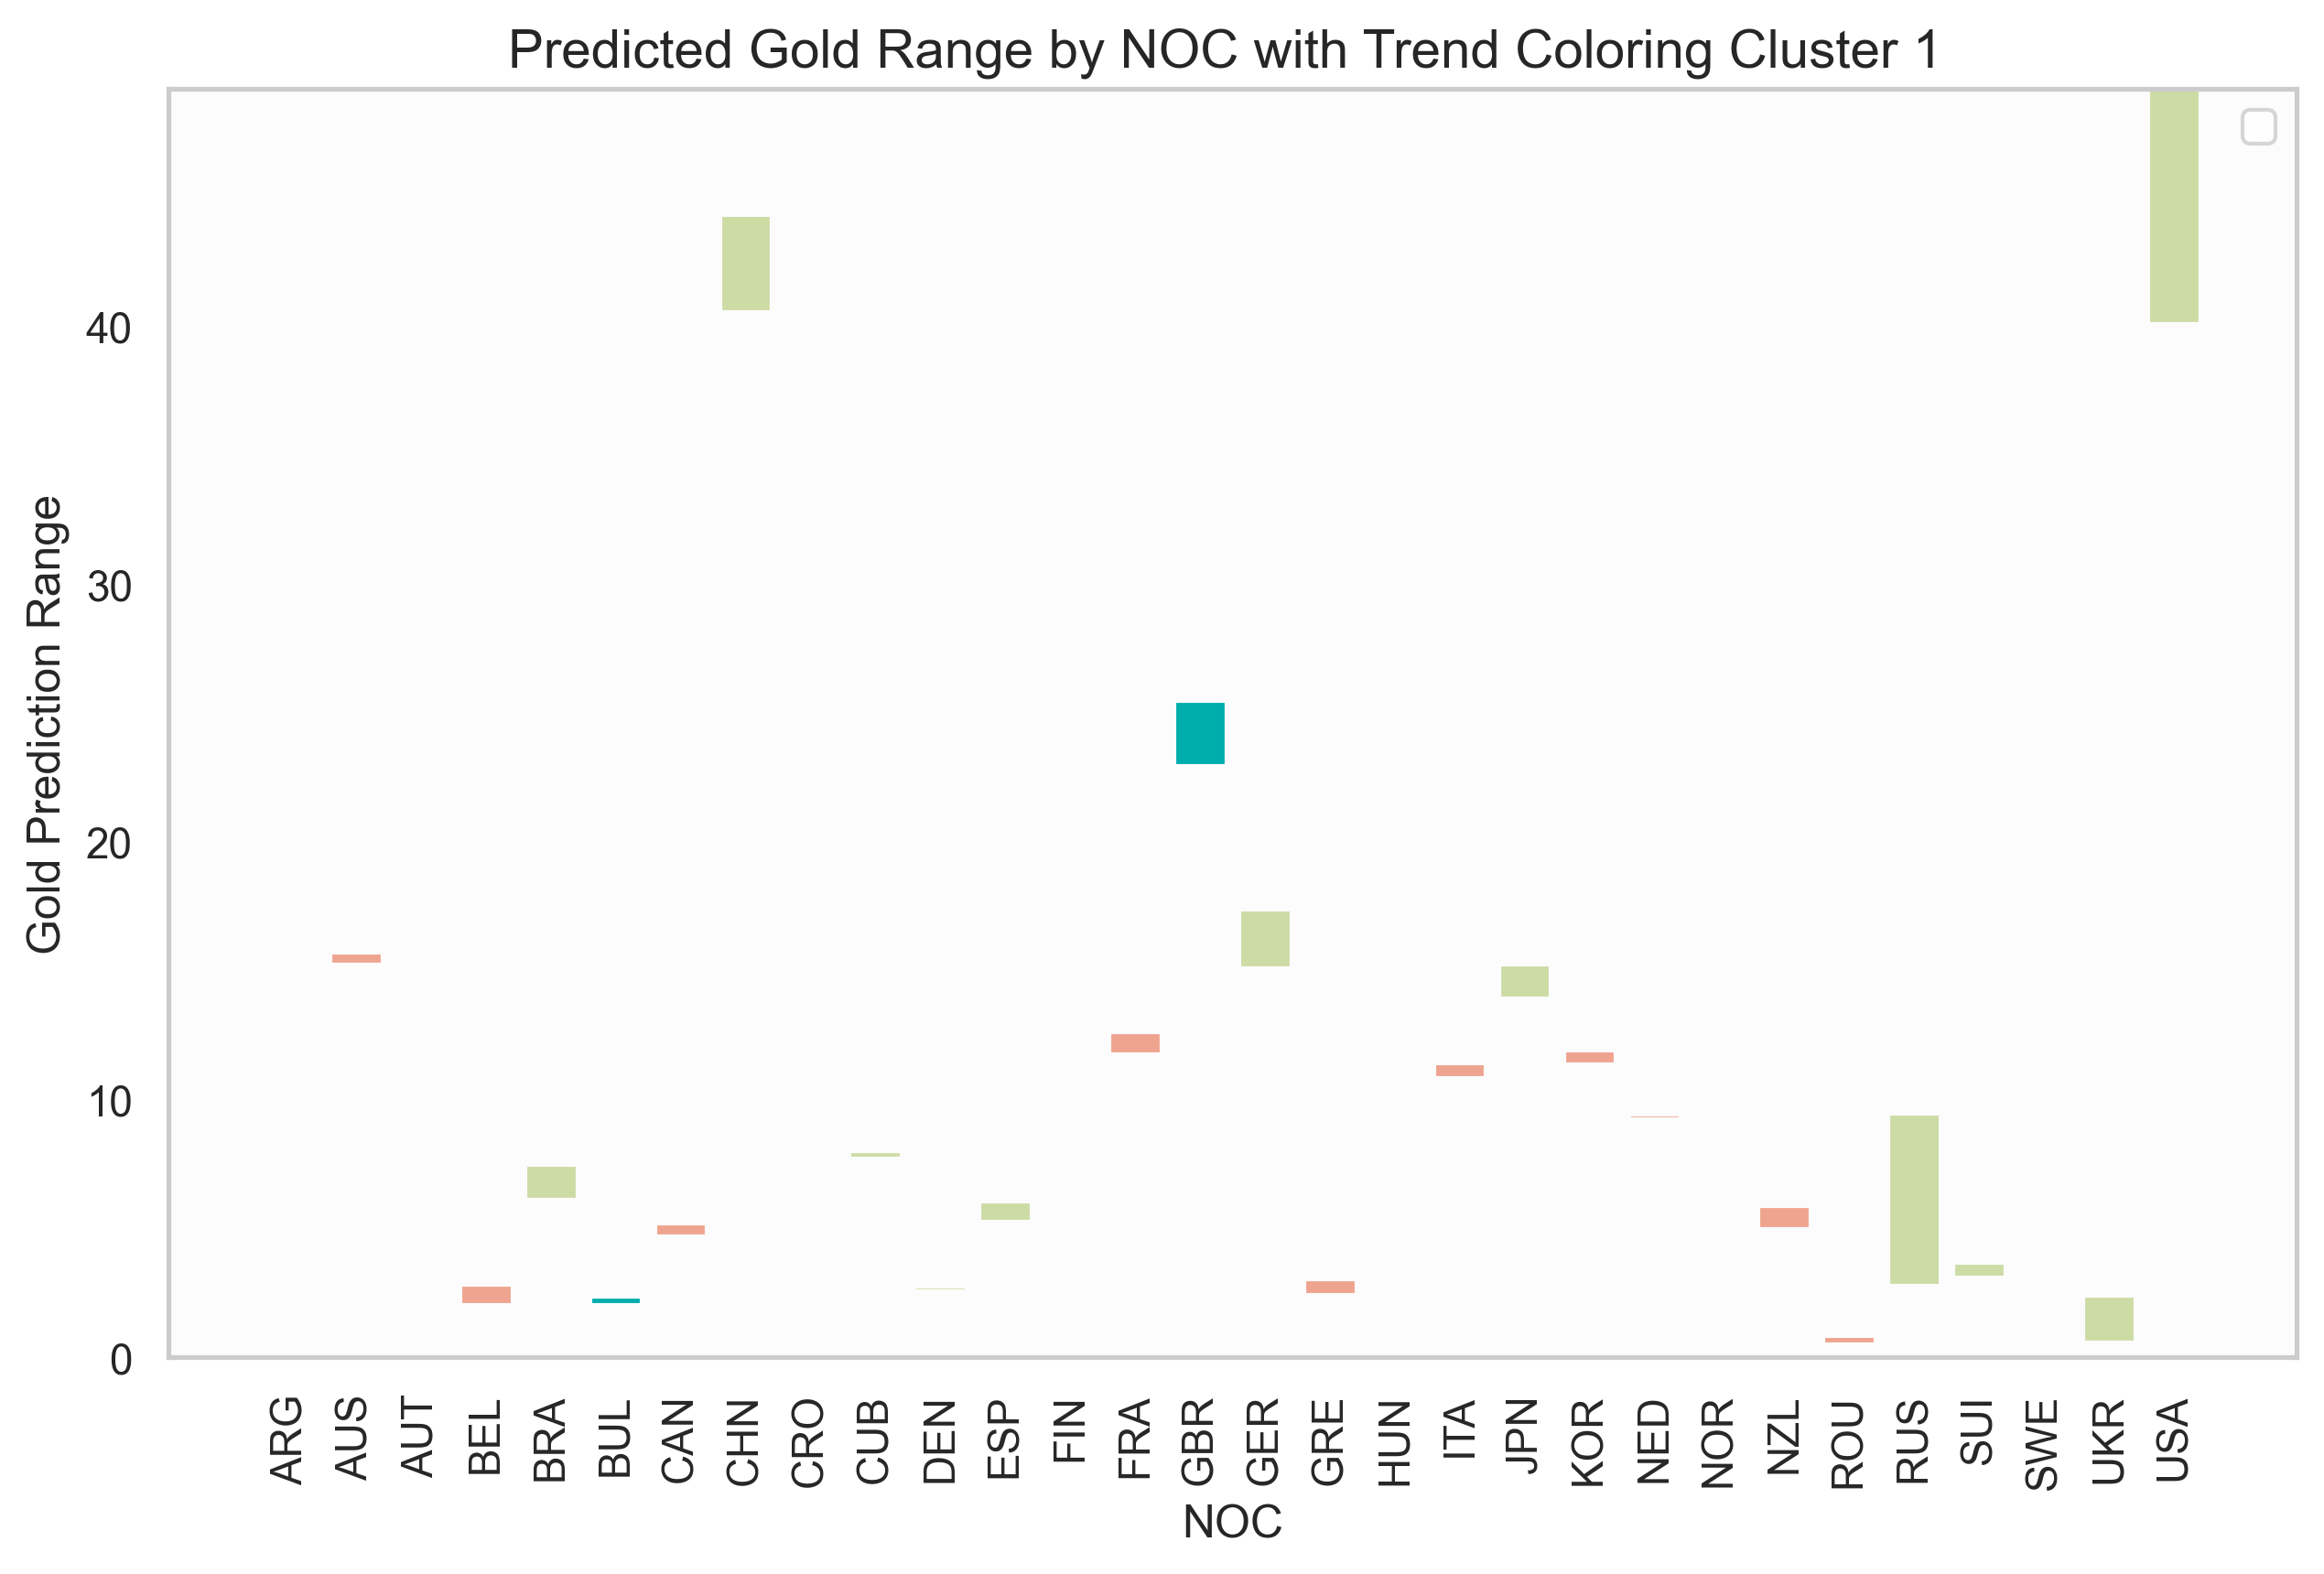
\includegraphics[width=.3\textwidth]{graph/res11.png}}
	\subfloat[Category 2] {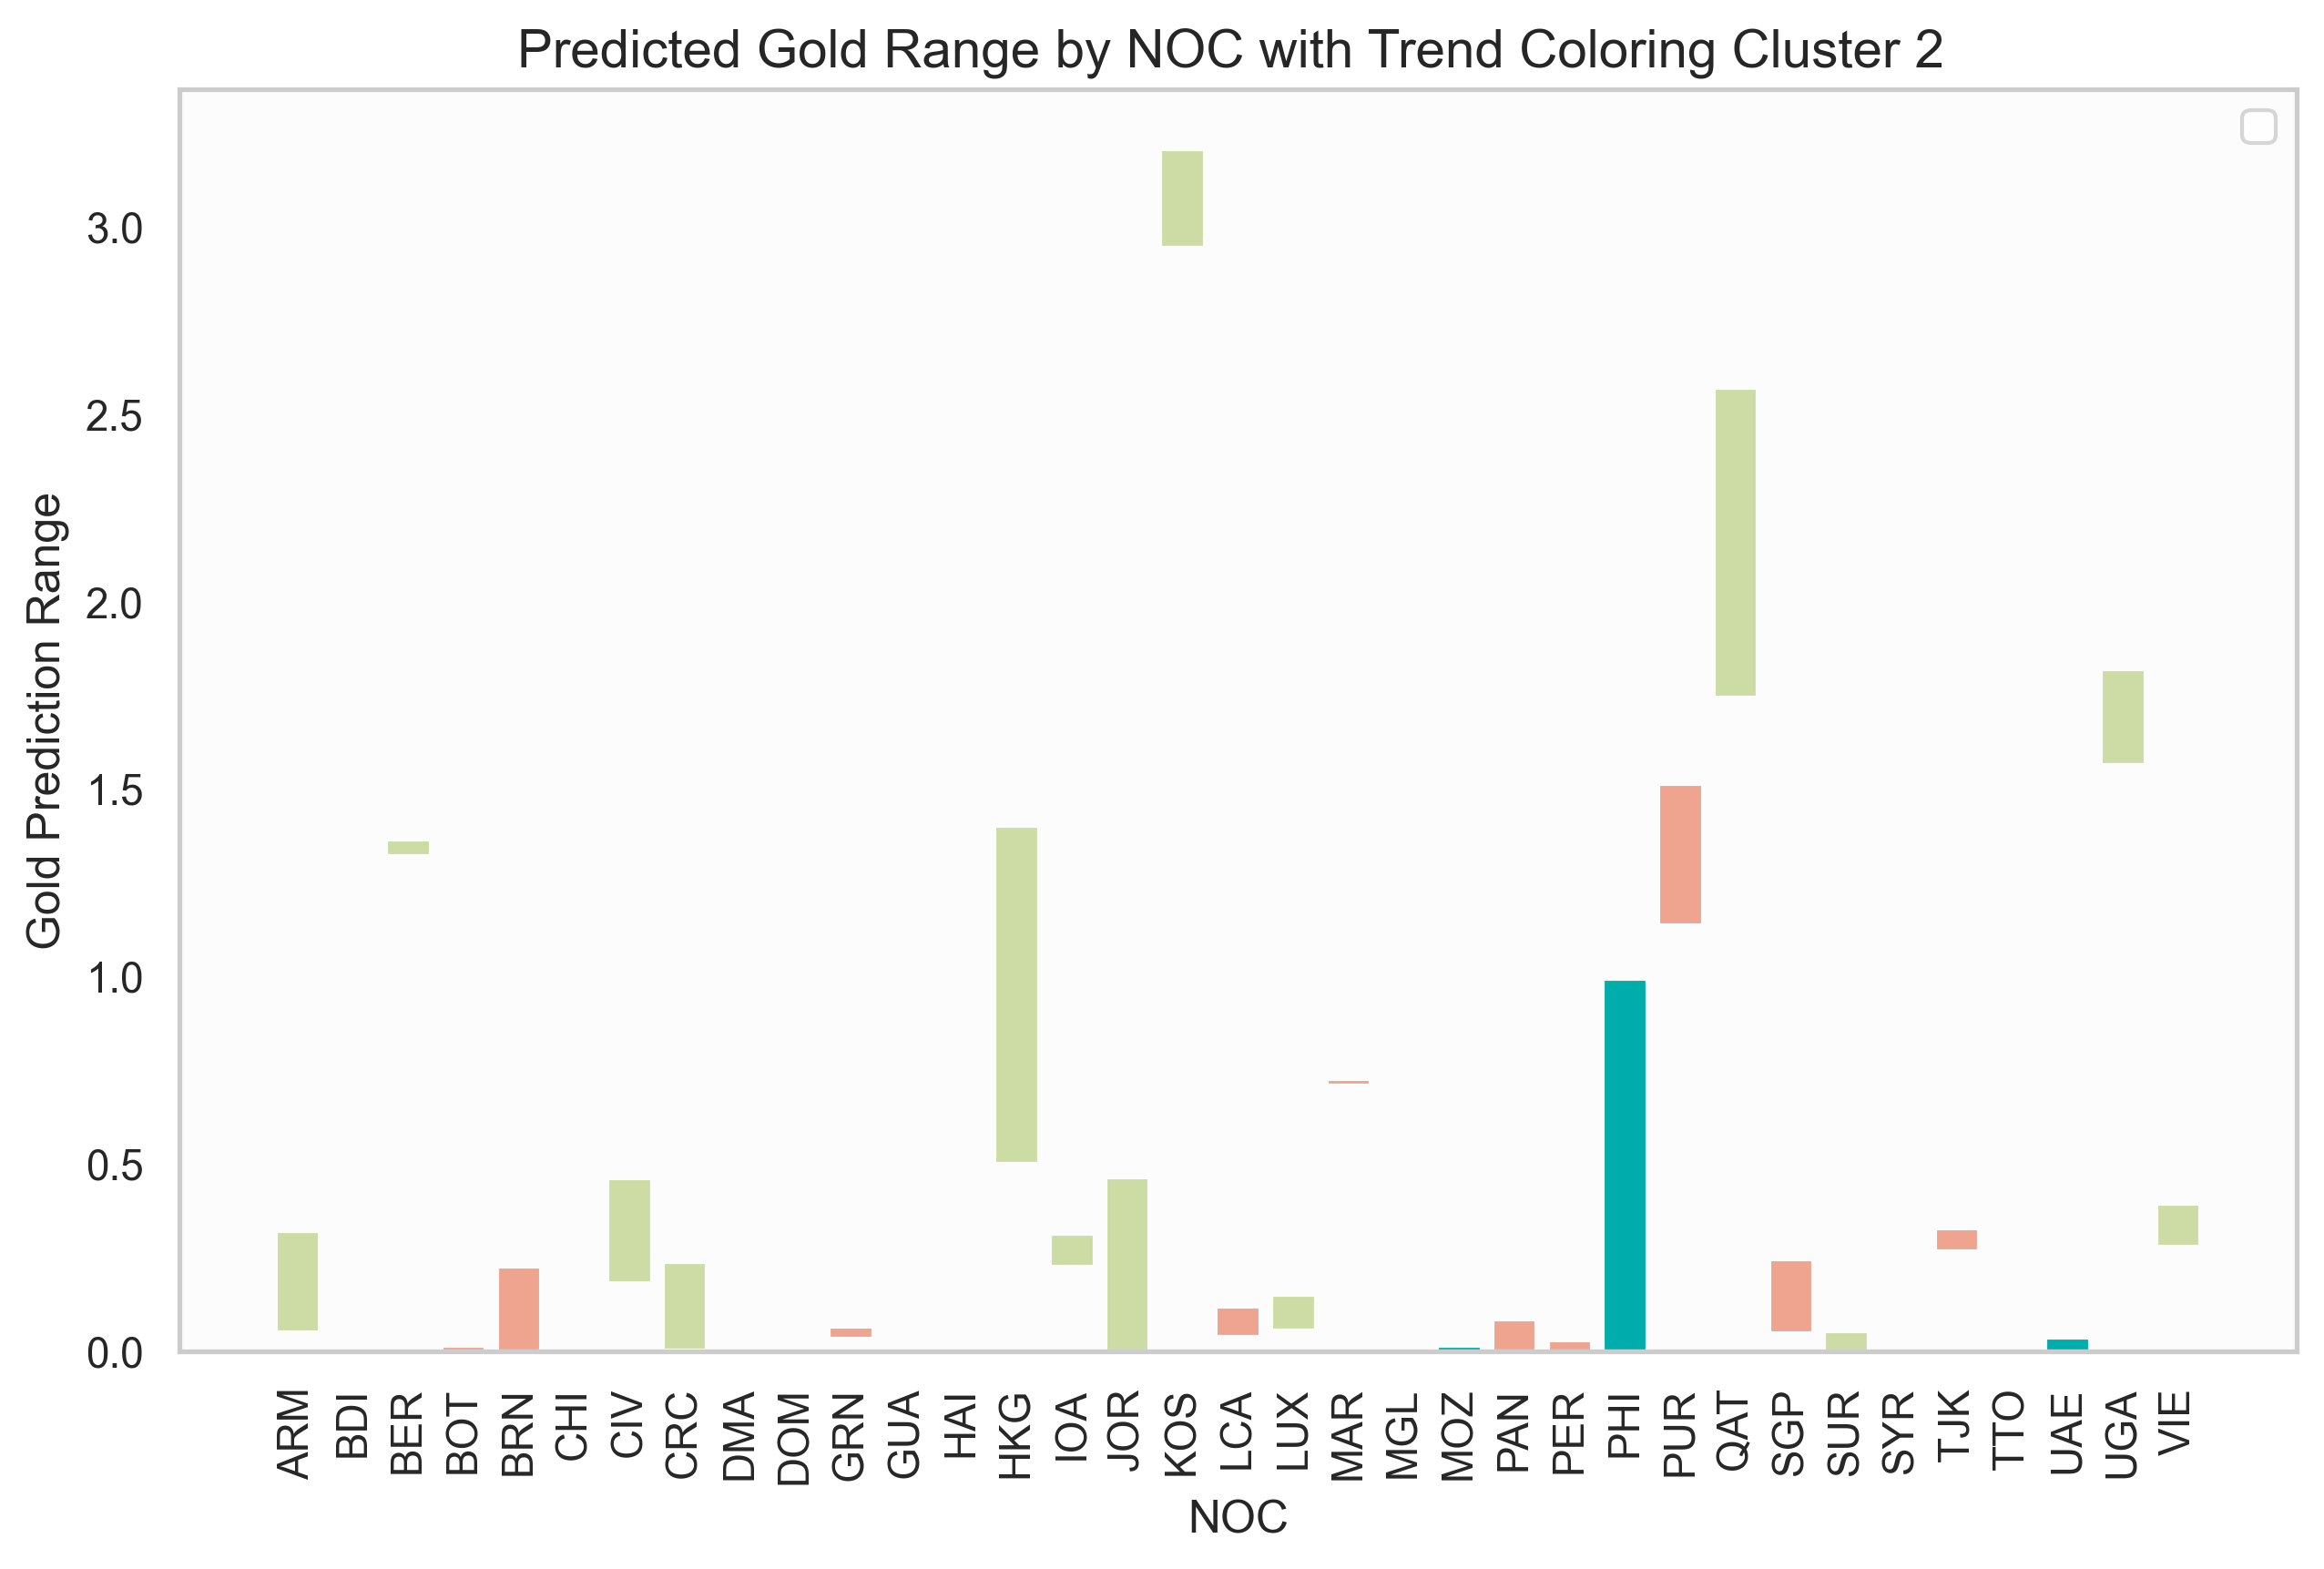
\includegraphics[width=.3\textwidth]{graph/res22.png}}
	\subfloat[Category 3] {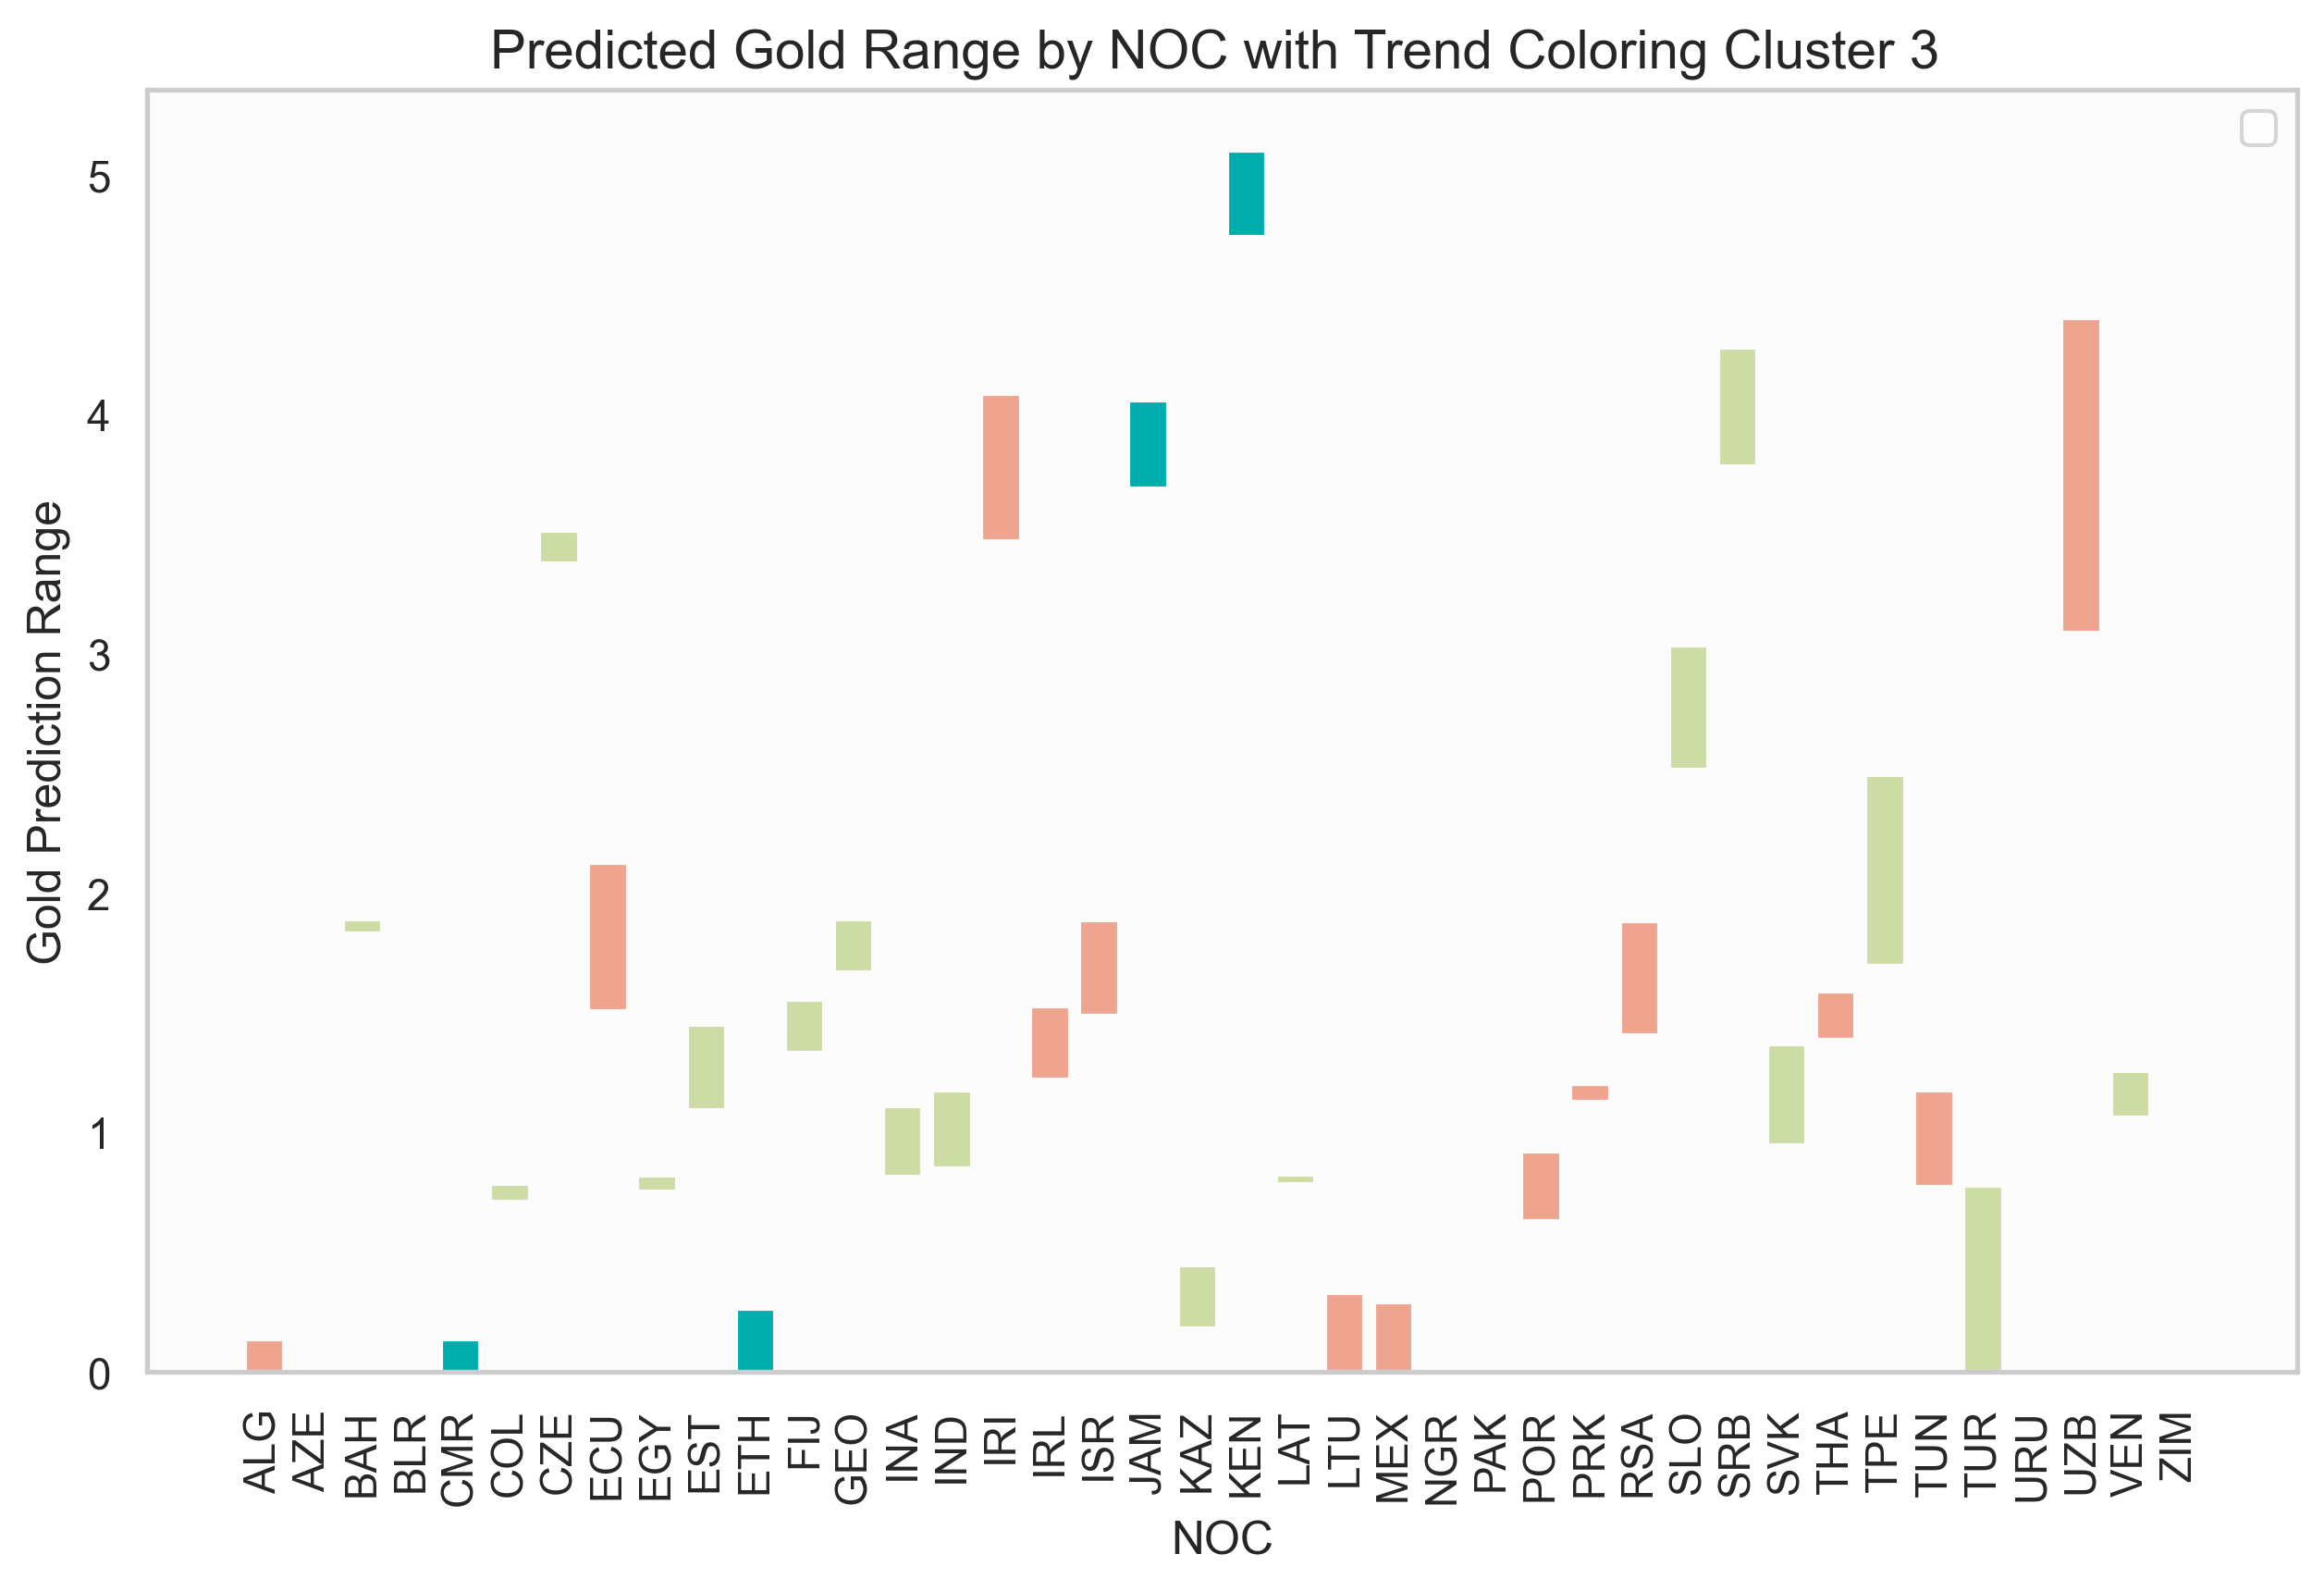
\includegraphics[width=.3\textwidth]{graph/res33.png}}
	\caption{Gold Medal Predictions for Category 3 Countries}
	\label{fig_E1}
\end{figure}

As shown in the figure above, 73 countries, represented by the United States and China, are expected to see an increase in medal counts, while 47 countries, represented by Australia and Canada, are expected to experience a decrease.

We analyzed the newly added events in previous Olympic Games and conducted a Pearson correlation analysis by combining the total historical medal counts of host countries in these new events with their overall medal counts. The results showed an average Pearson correlation coefficient of 0.4489306, indicating that the selection of new events by host countries has a significant impact on their overall medal count.

\begin{figure}[H]
    \centering
    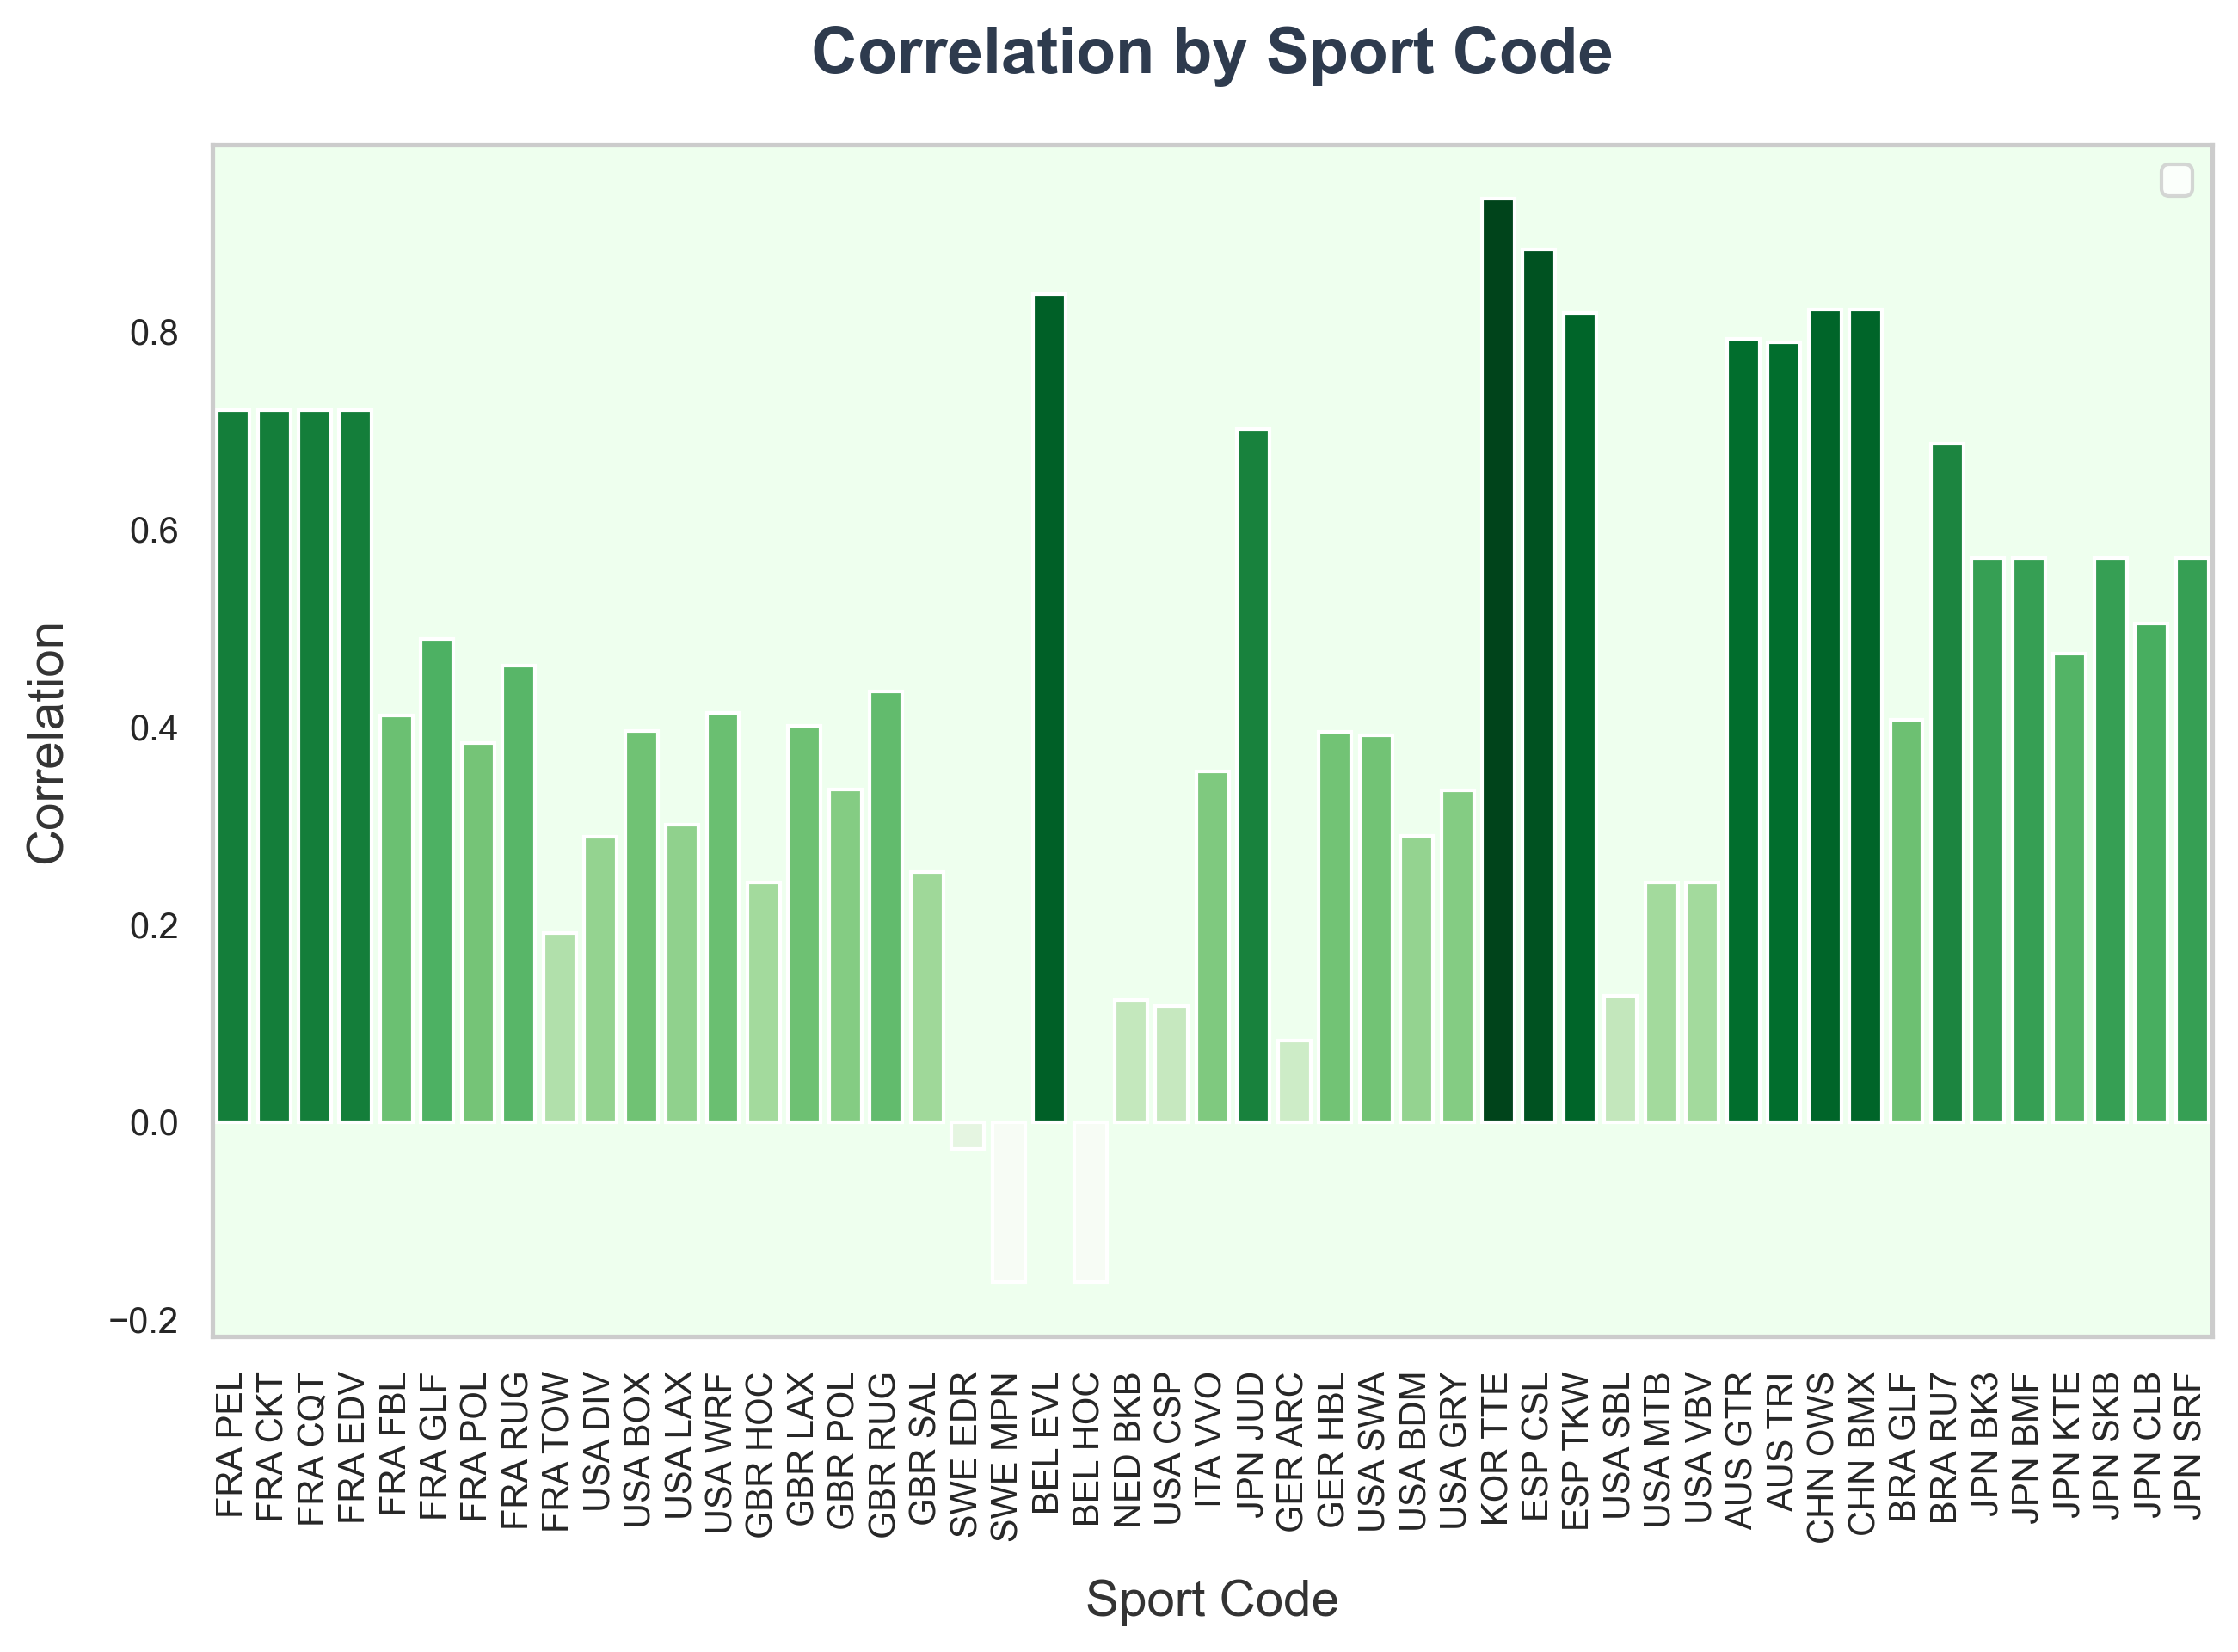
\includegraphics[width=12cm]{graph/Correlation by Sport Code.png}
    \caption{Correlation by Sport Code} \label{Figure 4}
\end{figure}

\subsection{the Advantage of LSTM}
The prediction of final medal counts using the LSTM model is typically not solely based on the time series of historical medal counts but rather considers multiple factors comprehensively, allowing for the analysis of both historical factors and the influence of advantage sports. To evaluate the advantages of the LSTM model in Olympic medal prediction tasks, we conducted a comparative experiment with the traditional Hidden Markov Model (HMM). By comparing the mean squared error (MSE) between the predicted results and actual values on the test set for both models, we observed that the LSTM model demonstrated significant superiority, with its prediction error being notably lower than that of the HMM model, as shown in Figure 11

\begin{figure}[htbp]
    \centering
    \begin{subfigure}{0.45\textwidth}
        \centering
        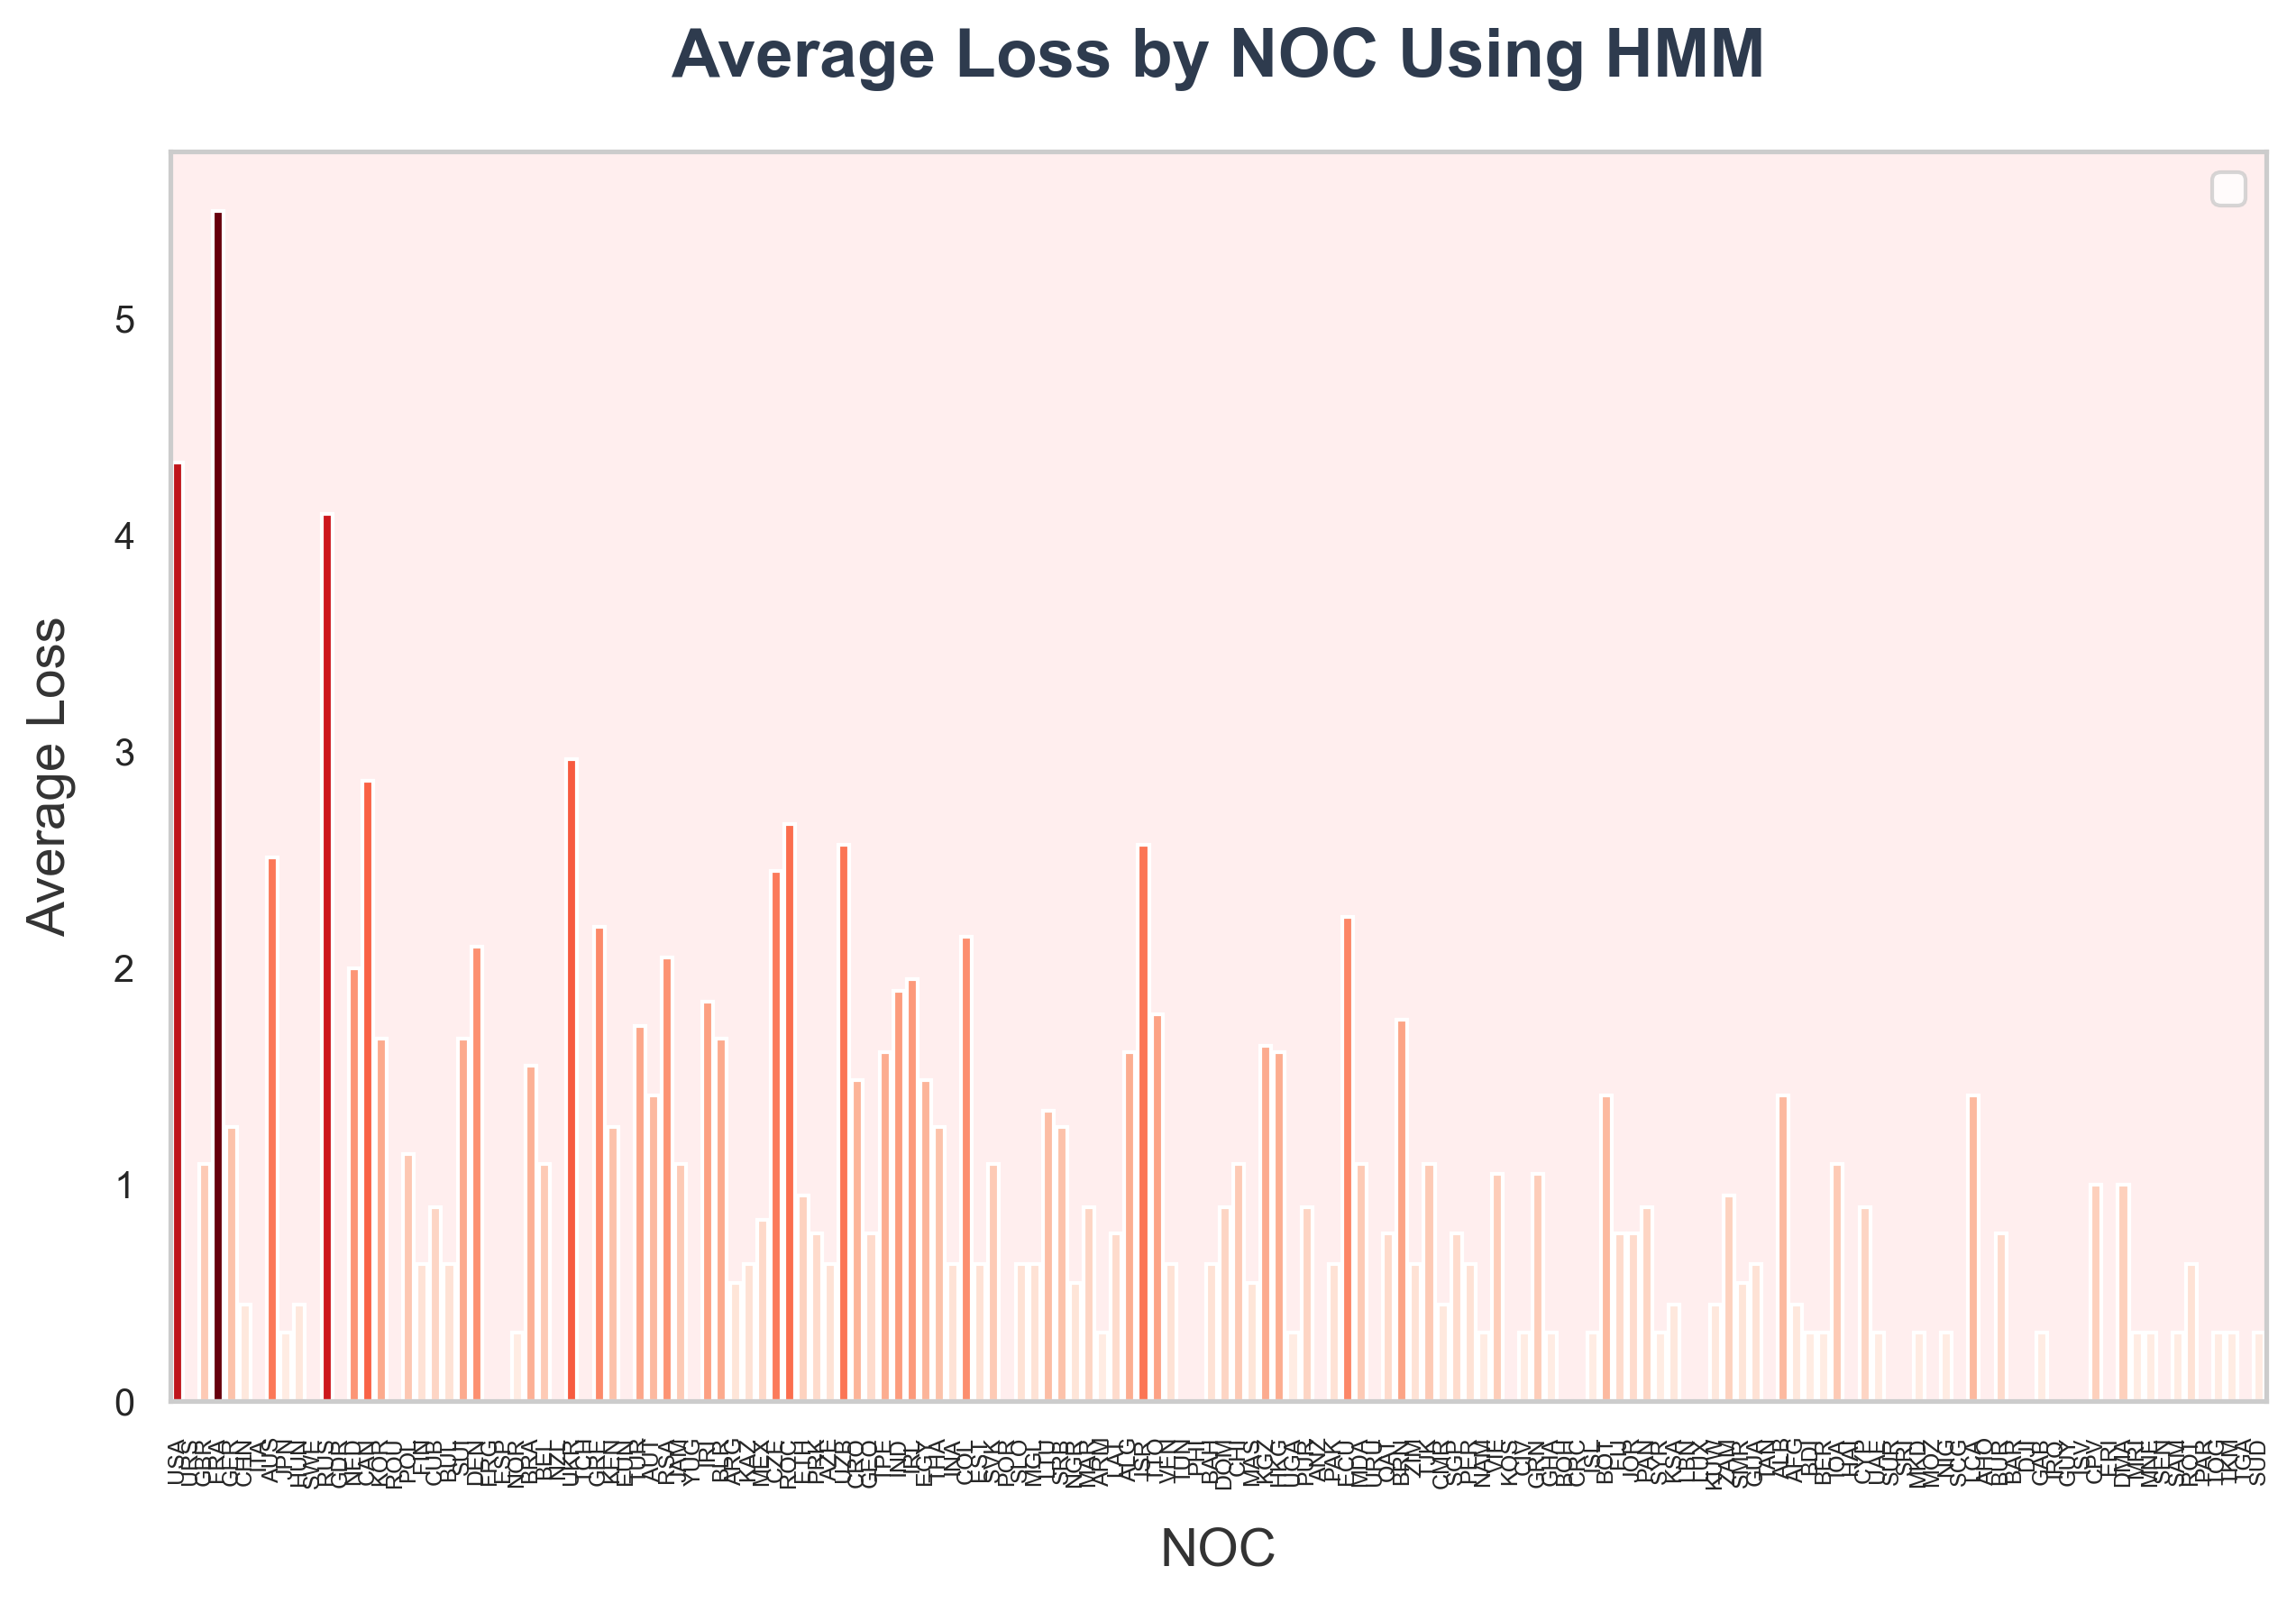
\includegraphics[width=\textwidth]{graph/Average Loss by NOC Using HMM.png}
        \caption{Average Loss by NOC Using HMM}
        \label{subfig:player1}
    \end{subfigure}
    \hfill
    \begin{subfigure}{0.45\textwidth}
        \centering
        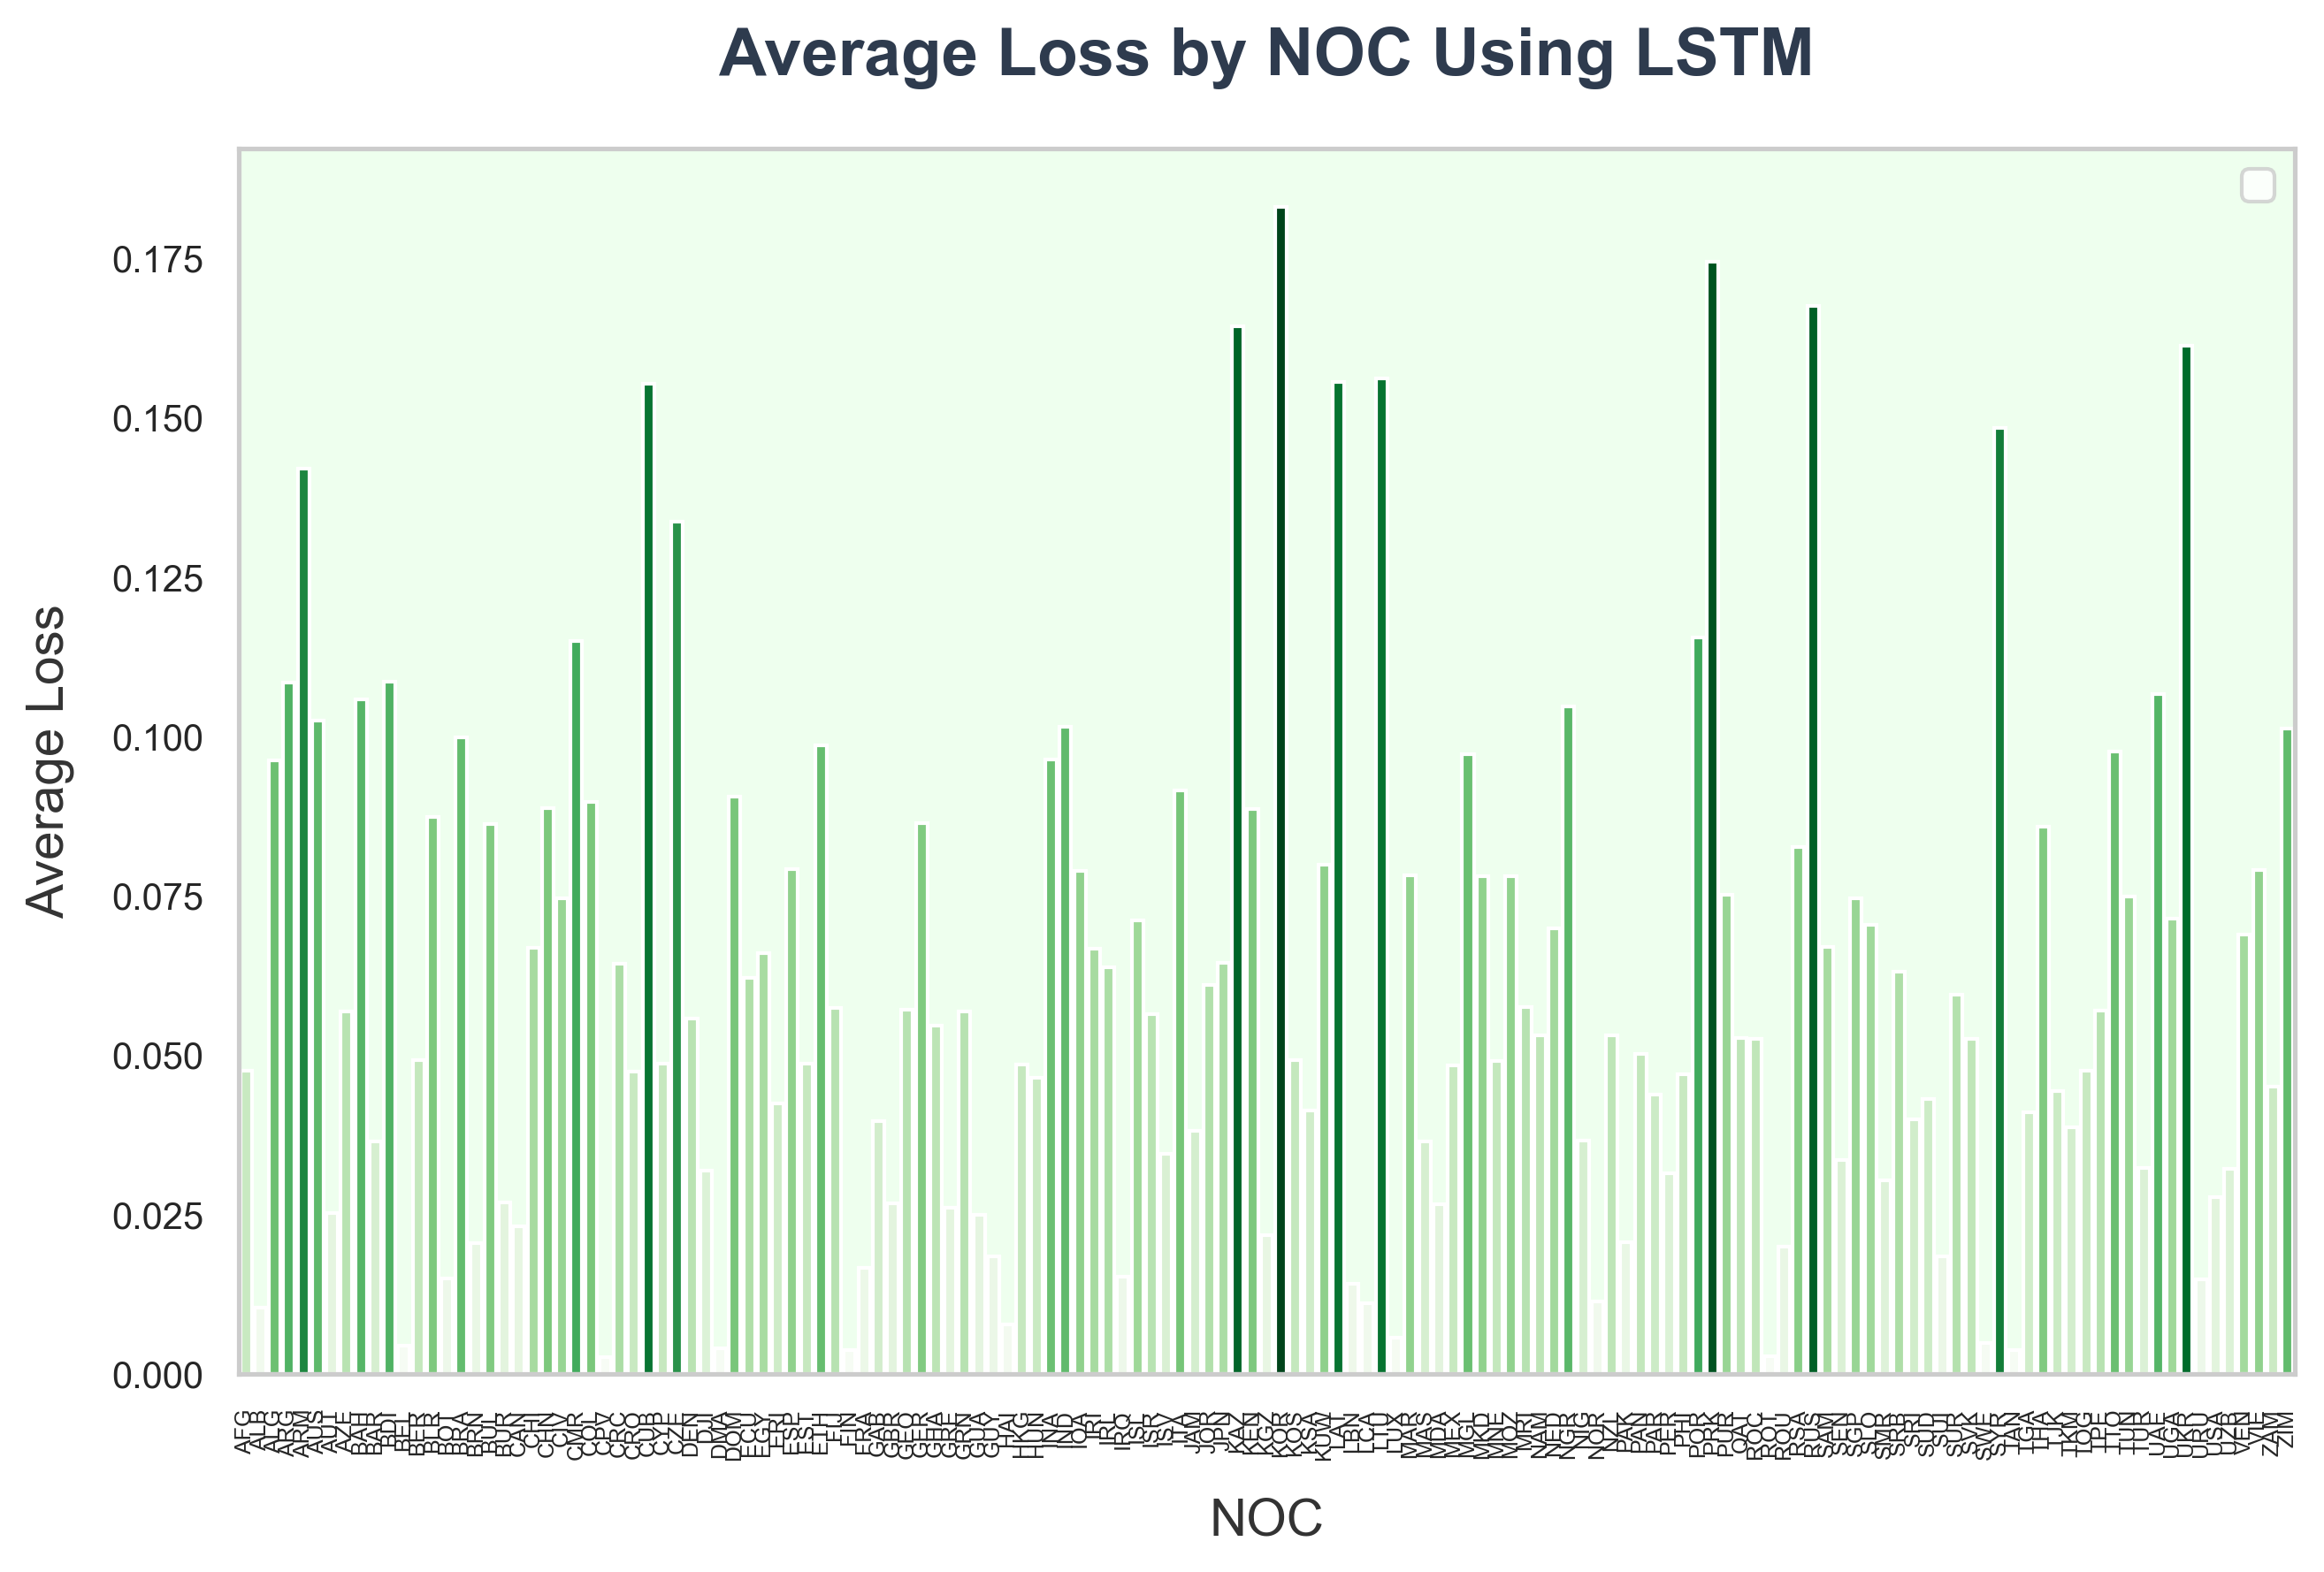
\includegraphics[width=\textwidth]{graph/Average Loss by NOC Using LSTM.png}
        \caption{Average Loss by NOC Using LSTM}
        \label{subfig:player2}
    \end{subfigure}
    \caption{Comparison of Medal Predictions Between HMM and LSTM Models}
    \label{Figure6-7}
\end{figure}
From the figure, it is evident that compared to the traditional Hidden Markov Model (HMM), the LSTM model demonstrates significantly better performance in predicting Olympic medals. We attribute this to the following reasons:
\begin{itemize}
   \item  1.	{\bf Model Structure}:The gated mechanism of LSTM (including the Forget Gate, Input Gate, and Output Gate) allows the model to adaptively regulate the retention of historical information. This enables the LSTM model to capture the long-term stable growth trends in medal counts for Olympic powerhouses. In contrast, HMM is constrained by its Markov assumption, which only models dependencies between adjacent time steps, making it difficult to capture long-term evolutionary patterns. Additionally, HMM struggles to accurately analyze the probability of countries with very few historical medals winning again or predict the outcomes for countries with high medal volatility or reliance on advantage sports. As shown in the figure [Loss Comparison], the LSTM prediction curve aligns much more closely with the actual values compared to the HMM model.
\item 2.	{\bf Feature Representation Capability}:LSTM, through its memory cells, can integrate multiple dimensions of information simultaneously, including historical medal counts, event participation, athlete scale, and other key factors. This dynamic multi-dimensional feature fusion mechanism allows the model to more accurately predict complex phenomena such as host country effects and the rise of emerging sports nations. In contrast, HMM’s state-space representation capability is relatively limited.
\item 3.	{\bf Optimization Objective}:LSTM uses an end-to-end gradient descent training approach, which directly optimizes prediction errors. In comparison, HMM relies on parameter learning through maximum likelihood estimation, which introduces a mismatch between the training objective and the actual prediction task. This discrepancy is a significant reason why LSTM demonstrates superior robustness in experiments.

\end{itemize}

%%%%%%%%%%%%%%%%%%%%%%%%%%%%%%%%%%%%%%%随机森林%%%%%%%%%%%%%%%%%%%%%%%%%%%%%%%%%%%%%%%
\section{TASK3:Random Forest-based prediction of first-time award-winning countries}

\subsection{Random Forest Model}
To identify the key factors influencing the transition in the number of medals won by a country, two steps are required:
\begin{itemize}
\item {\bf First}, a predictive model is developed to predict the turning point where the number of medals shifts from zero to one.        
\item {\bf Second}, infer key indicators based on the model results.
\end{itemize}

\subsection{Data Preparation and Preprocessing}

\subsubsection{Data Table Construction}
    Construct three data tables, participation\_by\_year\_country, participation\_by\_year\_country\_count, and sport\_count\_pivot, to record the number of participants of the country each year, the cumulative number of participations by year, and the number of events participated each year, respectively.

    To exclude countries that did not win any medals, entries from the participation\_by\_year\_country table corresponding to countries listed in the NOC column of the medal\_counts table were deleted.

    In the medals\_by\_year and medals\_by\_year\_gold datasets, the historical data for each country was traversed to determine the year in which they first won a medal. If all values in a column were zero, None was returned. The results were then stored in first\_medal\_filtered for preview. This dataset only contains countries whose first medal or gold medal year is greater than or equal to 1920.

\subsubsection{Dataset Creation}

{\bf First Iteration:}
    For each country's NOC, corresponding information was extracted from the participation\_by\_year\_country\_count, participation\_by\_year\_country, and sport\_count\_pivot data frames:
\begin{itemize}   
\item {\bf participation\_count:} The number of times the country participated in the year it first won a medal.
\item {\bf events\_participation} The number of events the country participated in during the year it first won a medal.
\item {\bf sport\_count: }The number of sports the country participated in during the year it first won a medal.
These extracted values were then added to , which will serve as the basis for subsequent datasets.
\end{itemize}

These extracted values were then added to new\_table\_data, which will serve as the basis for subsequent datasets.

{\bf Second Iteration:}
    To obtain data from the four years prior to the first medal year, the data from the four years after the first medal year were subtracted.

{\bf Third Iteration:}
    For each country that had never won a medal, the country's NOC, participation\_count, events\_participation, and sport\_count were added to new\_table\_data as a list.

    Finally, the entire list of data stored in new\_table\_data was converted into a Pandas DataFrame. After filling in missing values and cleaning invalid data, the final dataset, tree\_dataset, was formed.

\subsection{ Model Construction}

\subsubsection{Variable Analysis}
After careful selection and consideration of the available limited data, we chose three feature variables to train the model. The detailed list of variables is as follows:

    \begin{table}[h] 
        \centering  
        \caption{Table of Variables}  
        \label{tab1} 
    \begin{tabular}{ll} 
        \toprule[2pt]
        \textbf{Indicator}  & \textbf{Descriptions} \\    
        \midrule [1pt]
        $participation\_count$ & The number of participants from the country\\
        $events\_participation\_count$ & The number of times the country participated\\
        $sport\_count$   & The number of sports in which the country participated each time \\
        \bottomrule[2pt]
    \end{tabular}
    \end{table}

    At the same time, our target variable is Will\_Earn\_Medal, which indicates whether a medal will be earned (1 or 0).

\subsubsection{Model Training}
   
    After standardizing the data using StandardScaler, the dataset was split into training and testing sets, with 80\% used for training and 20\% for testing.

    We utilized the aforementioned features as input parameters for the Random Forest model to train on the training set. The parameter grid for the Random Forest model was as follows:
    \begin{table}[h] 
        \centering  
        \caption{Input parameters for forest models}  
        \label{tab1} 
    \begin{tabular}{ccccc} 
        \toprule[2pt]
        \textbf{Indicator}  & \textbf{Descriptions} \\    
        \midrule [1pt]
        $Number of Estimators$ & [50, 100, 150, 200]\\
        $Max Depth$ & [None, 10, 20, 30]\\
        $Min Samples Leaf$   & [2, 5, 10] \\
        $Min Samples Split$ & [1, 2, 4]\\
        $Max Features$ & ['auto', 'sqrt', 'log2']\\
        \bottomrule[2pt]
    \end{tabular}
    \end{table}

    We employed the RandomForestRegressor algorithm from the scikit-learn (sklearn) machine learning library, along with the GridSearchCV method for hyperparameter tuning. The optimal hyperparameter combination obtained from GridSearchCV was as follows:

    \begin{table}[h] 
        \centering  
        \caption{Optimal hyperparameter combination}  
        \label{tab1} 
    \begin{tabular}{ccccc} 
        \toprule[2pt]
        \textbf{Indicator}  & \textbf{Descriptions} \\    
        \midrule [1pt]
        $Number of Estimators$ & 200\\
        $Max Depth$ & 10\\
        $Min Samples Leaf$   & 1 \\
        $Min Samples Split$ & 2\\
        $Max Features$ & sqrt\\
        \bottomrule[2pt]
    \end{tabular}
    \end{table}

\subsubsection{Model Performance Visualization}

    To assess the performance of the mod

\begin{itemize}   
    \item {\bf Confusion Matrix} :Displays the relationship between the model's predictions and the true labels, helping to analyze the types of errors made by the model.
    \item {\bf ROC Curve}: Plots the Receiver Operating Characteristic (ROC) curve, which measures the model's performance across different thresholds.
\end{itemize} 

    The confusion matrix and ROC curve are shown below:

\begin{figure}[H]
    \centering
    \begin{subfigure}{0.4\textwidth}
        \centering
        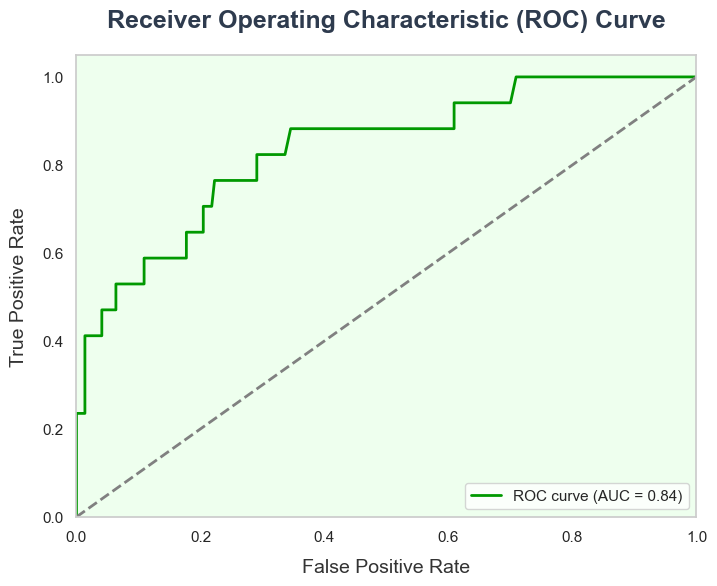
\includegraphics[width=\textwidth]{graph/rf_roc.png}
        \caption{ROC Curve}
        \label{subfig:player1}
    \end{subfigure}
    \hfill
    \begin{subfigure}{0.4\textwidth}
        \centering
        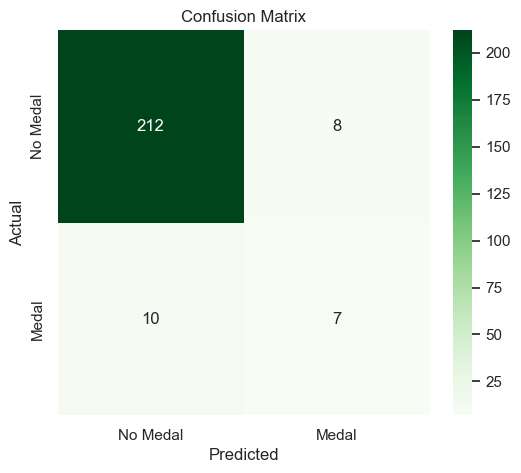
\includegraphics[width=\textwidth]{/graph/rf_confusion_matrix.png}
        \caption{Confusion Matrix}
        \label{subfig:player2}
    \end{subfigure}
    \caption{Model Performance Visualization}
    \label{Figure 13}
\end{figure}

    The confusion matrix indicates that the model's prediction accuracy is 94\%, with a false positive rate of only 0.039 (9/233), suggesting that the model is highly reliable and that most samples are correctly classified. The match between the predicted values and the true labels in the test set is high.

    The model's AUC (Area Under the Curve) is 0.87, demonstrating strong discriminative power and the ability to effectively distinguish between positive and negative classes. Additionally, the ROC curve rapidly rises in the low false positive rate (FPR) region, indicating that the model achieves a high recall rate while maintaining a low false positive rate. The model's true positive rate is commendable.

\subsubsection{Model Prediction}
    Using the best-trained model, {\bf best\_rf\_model}, we predicted the outcomes for new standardized data. The predict\_proba() method returns the probability of each sample belonging to each class, which allows us to calculate the probability of each country winning a medal.

\subsection{Model Testing}

\subsubsection{Test Set Construction}

    To validate the model's performance in real-world prediction tasks, we identified and selected historical samples of countries that have never won a medal from the {\bf athletes} dataset. We used a temporal grouping method to ensure the continuity and completeness of the data. After standardizing the feature data and applying quality control measures, we ultimately formed a high-quality test dataset.

    A new dataset containing relevant statistical data for all countries that have never won a medal was generated for the year 2024.

\subsubsection{Testing}

    Using the trained Random Forest model {\bf best\_rf\_model}, we predicted the features for each country and calculated the probability of each country winning a medal. These probabilities were stored in a list, sorted, and the countries most likely to win a medal were identified. A bar chart was then generated to visualize the predicted probabilities of each country winning a medal.

    Through probability distribution analysis, it was found that the prediction results exhibit distinct layering. Countries with a predicted probability greater than 0.20 are primarily concentrated in emerging market nations with well-developed sports infrastructure. These countries generally show consistent investment in sports and the specialization of sports programs.

\begin{figure}[h]   
    \centering          
    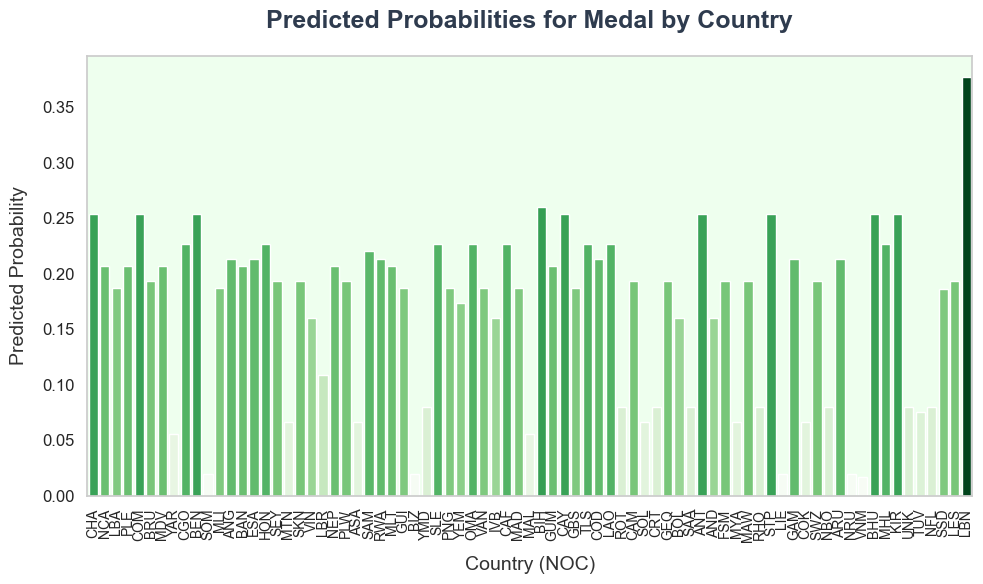
\includegraphics[width=12cm]{graph/rf_prediction.png}
    \caption{Predicted Probabilities for Medal by Country} \label{fig1}    
\end{figure}





%%%%%%%%%%%%%%%%%%%%%%%%%%%%%%%%%%%%%%%伟大教练%%%%%%%%%%%%%%%%%%%%%%%%%%%%%%%%%%%%%%%%
\section{TASK4: Quantitative Graph Theory Model of the "Great Coach Effect" Based on Network Flow}
\subsection{Model Background}
In international competitions such as the Olympic Games, athletes' nationalities are typically restricted; however, coaches do not need to be citizens of the countries they coach. This allows them to move freely between countries. In certain cases, coach changes have had a significant impact on the performance of sports teams, especially when they have a "great coach effect." Such coaches may help teams or athletes break through performance barriers and improve results. The aim of this model is to verify the existence of the "great coach effect" through data analysis and quantify its contribution to medal counts.

In this section, we need to complete:
\begin{itemize}
    \item 	{\bf Data Analysis}: Explore whether coach changes are related to changes in medal counts in different countries and sports.
    \item	{\bf Model Construction}: Analyze the impact of the coach effect on medal counts through a network flow model based on graph theory.
    \item	{\bf Impact Prediction}: Identify which sports are suitable for investing in "great coaches" and analyze their potential impact
\end{itemize}

\subsection{Model Construction}
This section aims to construct a directed graph based on the network flow model of graph theory, which can effectively reflect how coach movement influences medal count changes in various countries. Through this model, we can quantify the coach’s influence, especially the impact on a country’s sports results after the coach's movement or replacement. The nodes in this graph represent different countries, while the directed edges represent the movement of coaches between countries and their contributions to medal counts. By applying the total flow and bottleneck flow algorithms, we can deeply analyze the coach's role, evaluate their impact on medal counts, and provide scientific recommendations for future coach selection and resource allocation.
\begin{figure}[h]   
    \centering          
    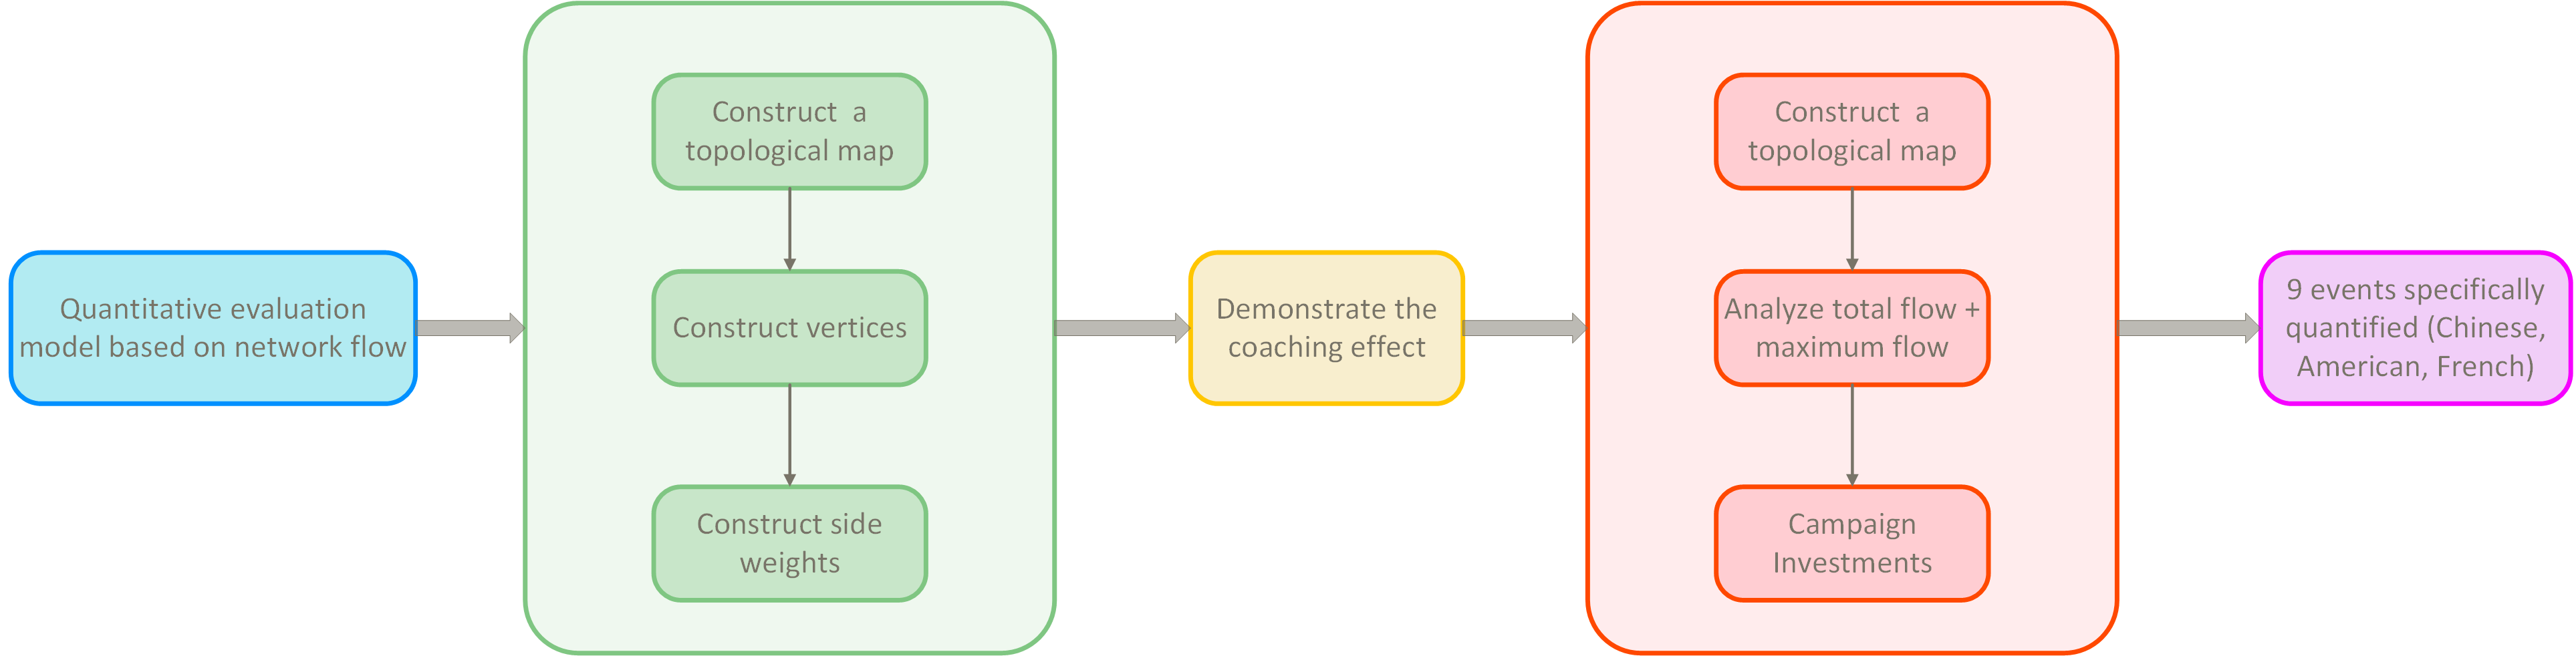
\includegraphics[width=12cm]{graph/graphy_baseline.png}
    \caption{Quantitative Evaluation Framework Based on Network Flow Model } \label{fig1}    
\end{figure}

\subsubsubsection{Construction of the Basic Directed Graph}
In the network flow model based on graph theory, we first build a basic directed graph that can reflect the movement of coaches. The nodes represent countries, while the directed edges represent the flow path of a coach moving from one country to another (with the Olympic Games as the time period). If the coach remains in the same country and participates in multiple Olympic Games, a self-loop edge can be used


\begin{figure}[H]
    \centering
    \begin{subfigure}{0.45\textwidth}
        \centering
        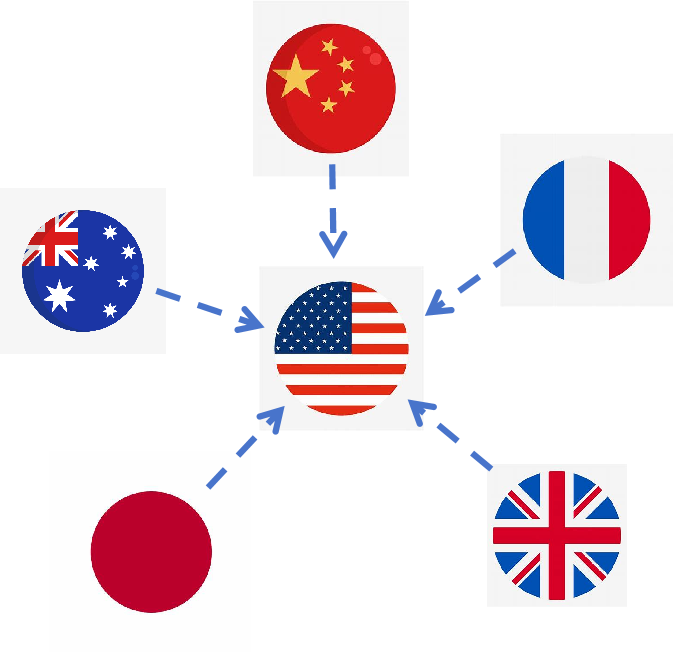
\includegraphics[width=\textwidth]{graph/graphy super country.png}
        \caption{super country type}
        \label{subfig:player1}
    \end{subfigure}
    \hfill
    \begin{subfigure}{0.45\textwidth}
        \centering
        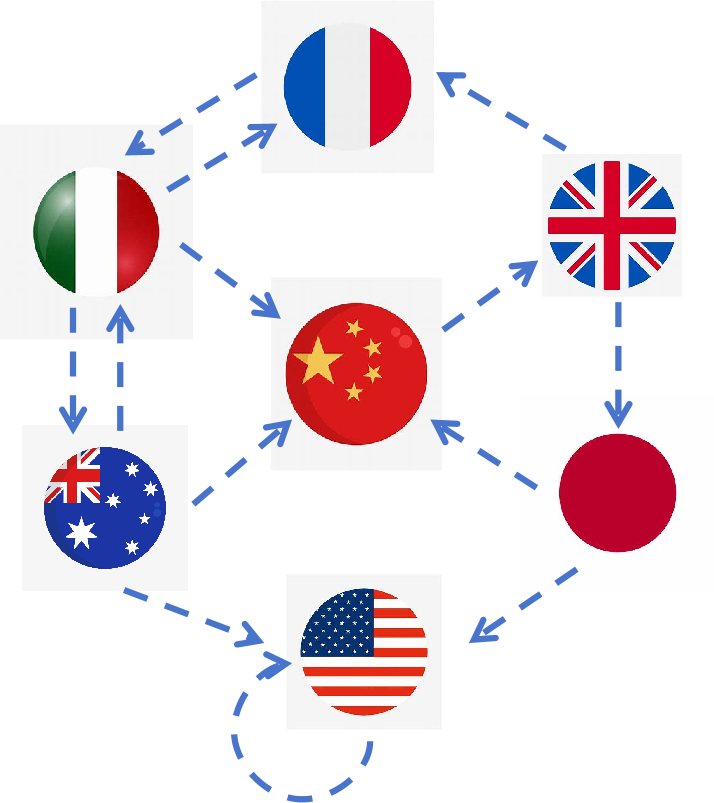
\includegraphics[width=\textwidth]{graph/graphy country flow.png}
        \caption{Large country circulation type}
        \label{subfig:player2}
    \end{subfigure}
    \caption{graph theory model}
    \label{Figure 13}
\end{figure}








%%%%%%%%%%%%%%%%%%%%%%%%%%%%%%%%%%%%%%%letter%%%%%%%%%%%%%%%%%%%%%%%%%%%%%%%%%%%%%%%%
\section{Letter}
Dear Sir or Madam
It is a great honour to write to you and share with you the results of our analysis of Olympic medal predictions. As a global platform for competition, the Olympic Games not only showcase the pinnacle of athletic excellence, but also foster international unity. In our mathematical modelling of Olympic medal predictions, we have identified several key findings, including trends in gender participation, the impact of host nations on medal counts, and the potential of under-researched sports.

These insights not only reflect historical and current trends but also provide actionable strategic recommendations for National Olympic Committees in their preparations for future Olympic events. 

Here are the detailed analyses of these findings and the implications for future planning:

1.Through statistical analysis of Olympic participation data, it was found that gender participation has shown significant evolutionary characteristics. In the early Olympic Games, male athletes dominated (accounting for approximately 70%), while in recent years, this proportion has gradually approached balance.

\begin{figure}[htbp]
    \centering
    \begin{subfigure}{0.45\textwidth}
        \centering
        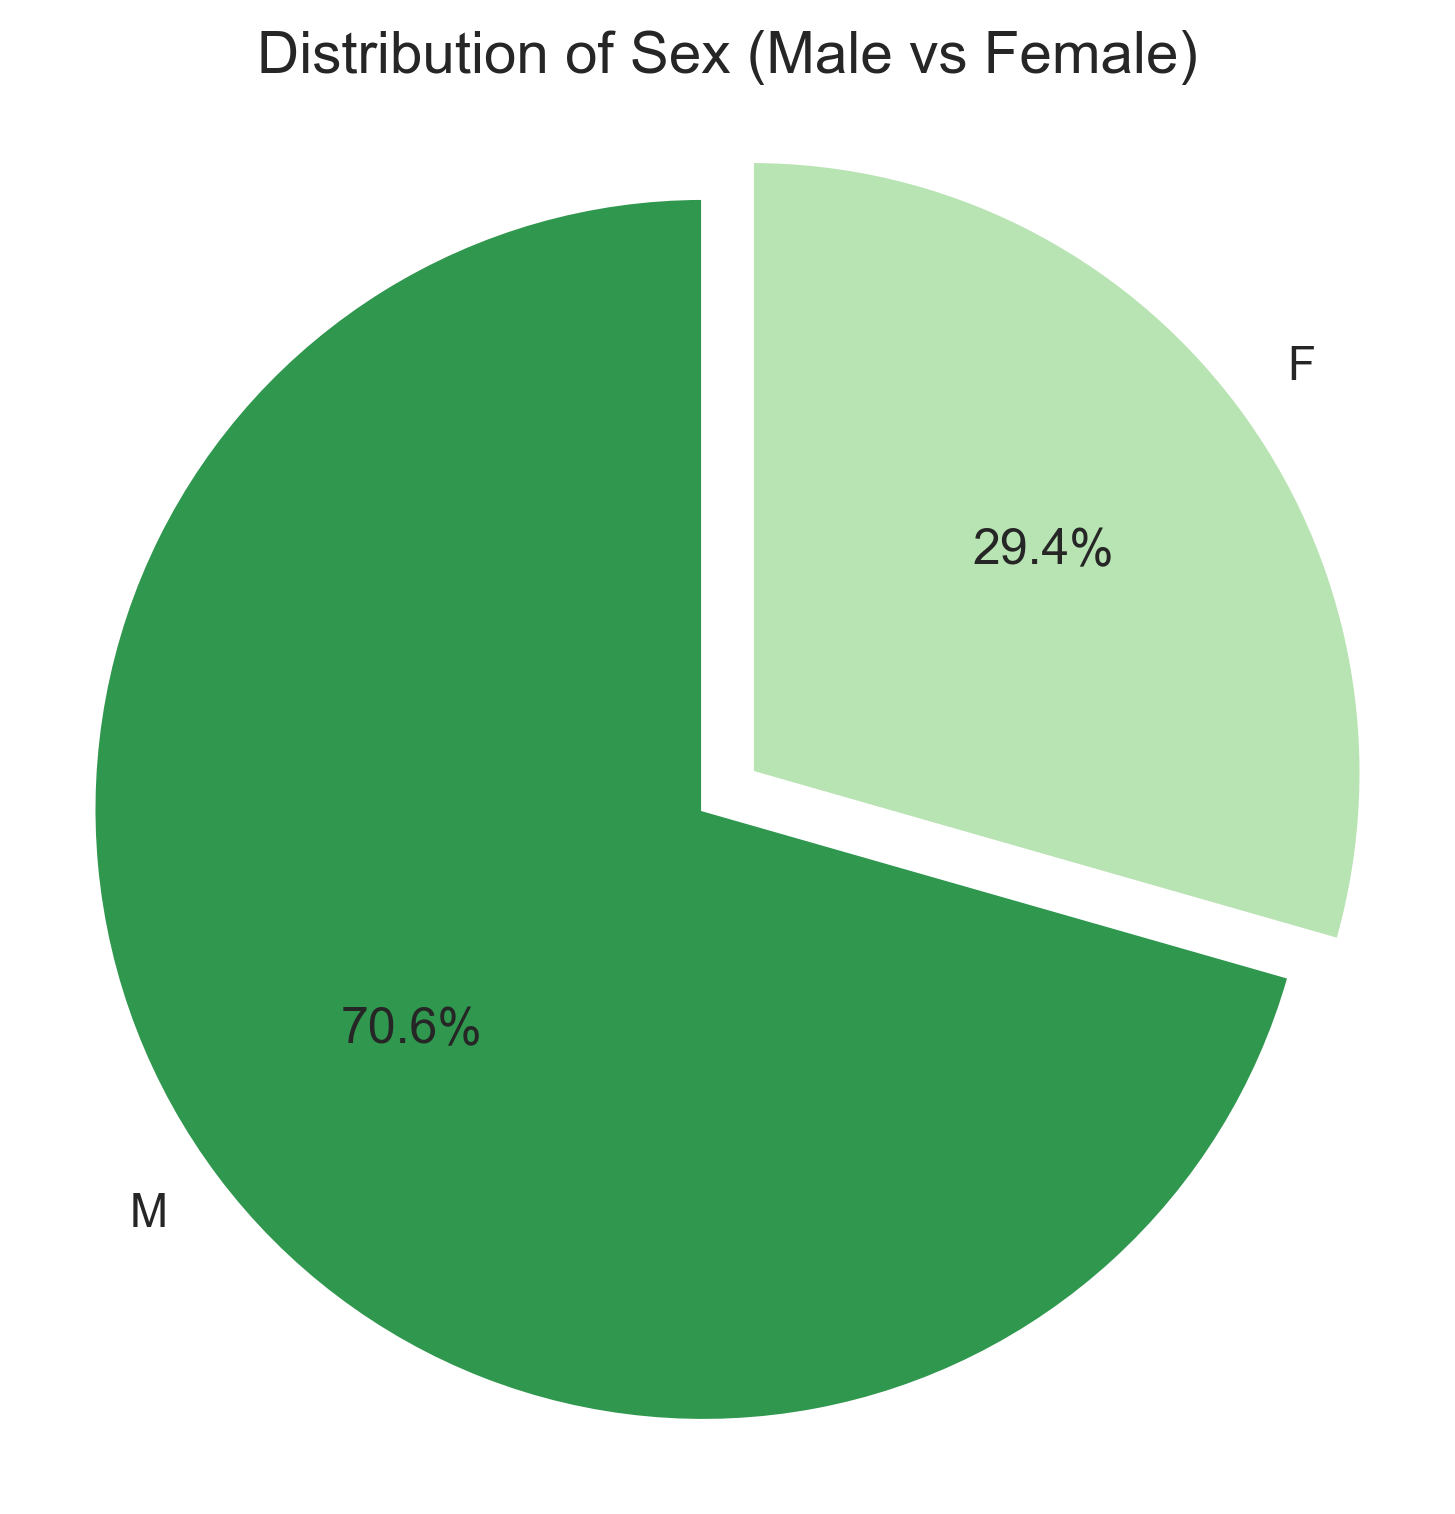
\includegraphics[width=\textwidth]{graph/Distribution of Sex.png}
        \caption{Distribution of Sex}
        \label{subfig:player1}
    \end{subfigure}
    \hfill
    \begin{subfigure}{0.45\textwidth}
        \centering
        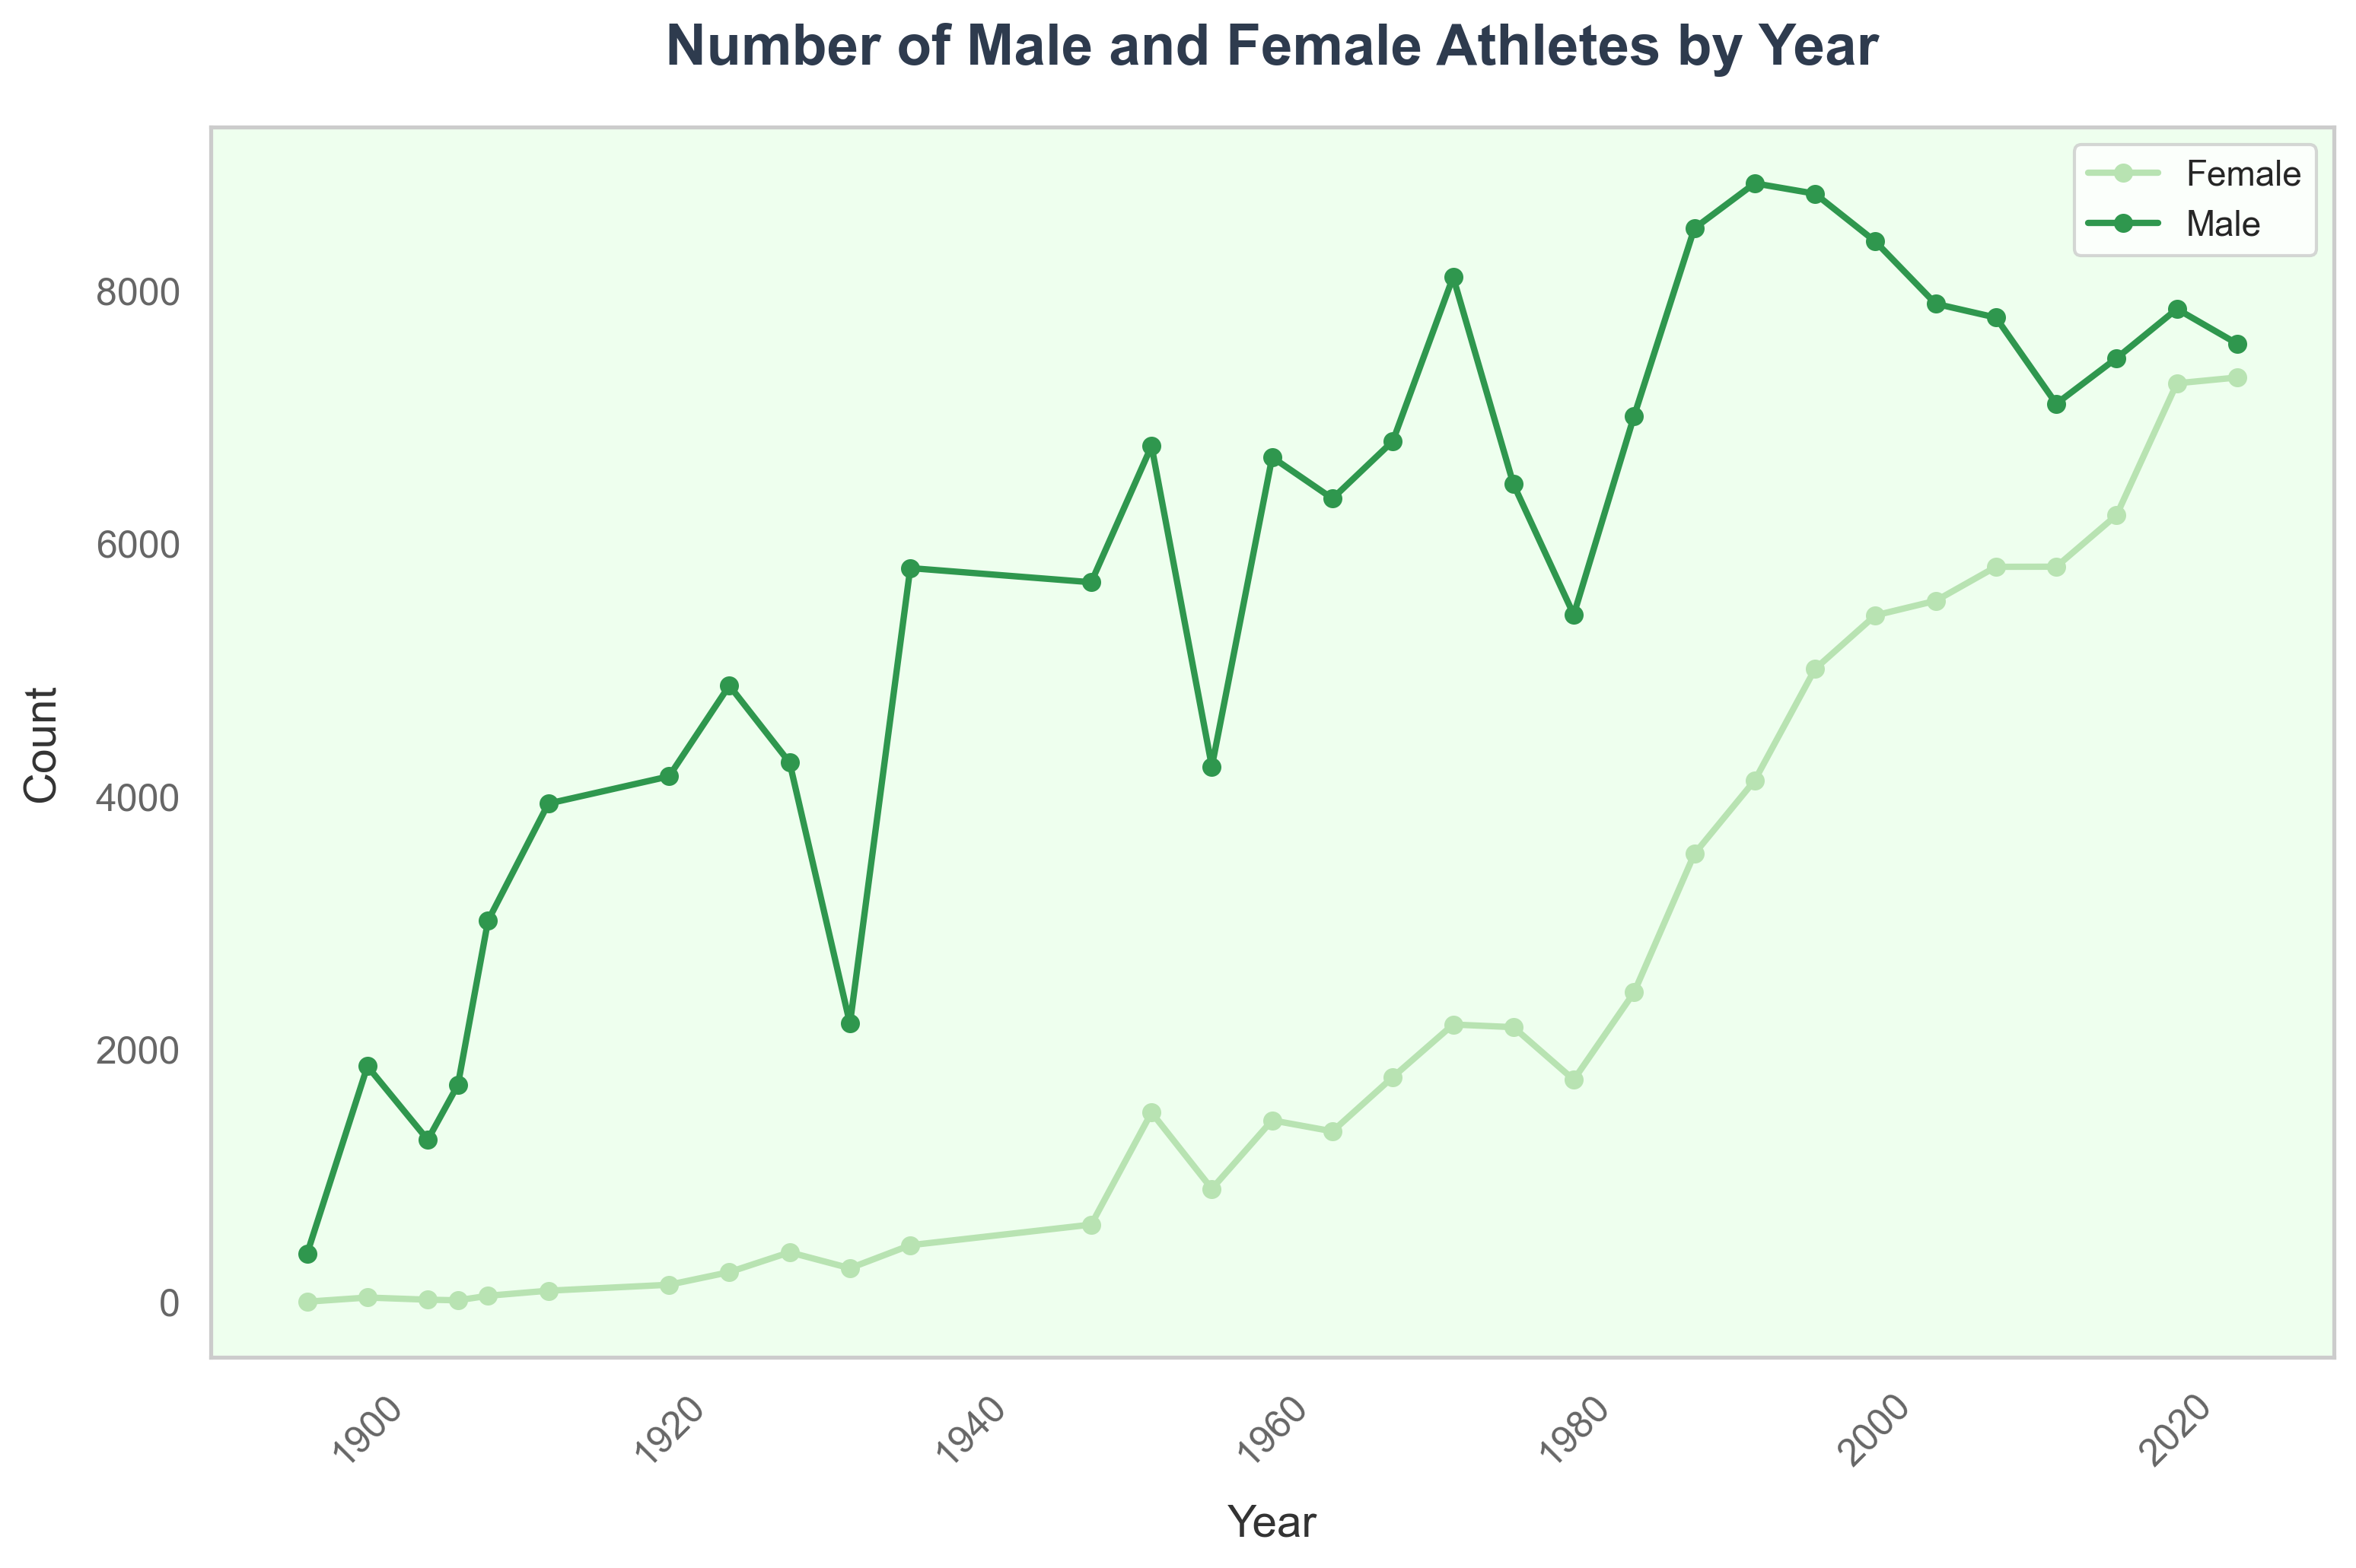
\includegraphics[width=\textwidth]{graph/Number_of_Athletes_by_Sex.png}
        \caption{Number of Athletes by Sex}
        \label{subfig:player2}
    \end{subfigure}
    \caption{Player 1/2's Momentum in this set}
    \label{Figure6-7}
\end{figure}
%%%%%%%%%%%%%%%%%%%%%%%%%%%%%%%%%%%%%%%模型分析%%%%%%%%%%%%%%%%%%%%%%%%%%%%%%%%%%%%%%%%
\section{Model Assessment}
\subsection{Strengths}
1.During the data analysis process, we comprehensively considered multiple key factors such as the number of participants, the number of events, hosts, and outstanding coaches. As a result, we conducted extensive data validation, and our predictions were not solely reliant on historical medal counts.

2.In building the model, we compared it with several other models, such as the Hidden Markov Model and Multivariate Logistic Regression, through experimental validation.

3.We applied various mathematical modeling techniques, including machine learning, neural networks, and graph theory, and flexibly adjusted variables and weights to adapt to medal predictions for different countries.
\subsection{Weaknesses}
1.During data cleaning, due to time constraints, we used the athletes dataset as the primary reference for valid NOCs and removed NOCs from the hosts and medals datasets that were not present in the athletes dataset. We did not consider historical changes in countries in greater detail.

2.The lack of data limited the ability to perform more multidimensional model validation. We excluded factors like GDP, and a multivariate linear regression could have better validated the "Great Coach" effect.
\end{document}